\documentclass[12pt,oneside,a4paper]{book}
\usepackage[latin1]{inputenc}
\usepackage[english, spanish]{babel} %For languages characters and hyphenation
\usepackage{amsmath}
\usepackage{amsfonts}
\usepackage{titlesec}
\usepackage{amssymb}
\usepackage{graphicx}
\usepackage{array}
\usepackage{cite}
\usepackage[all]{xy}
\usepackage{fancyhdr}
\usepackage{lastpage}
\usepackage{caption}
\usepackage{subcaption}
\usepackage{multicol}
\usepackage{tabularx}
\usepackage{hhline}
%\usepackage{subfig}
%\usepackage{subfigure}
\usepackage{multirow}
\usepackage[acronym]{glossaries}
\usepackage{microtype} % Makes pdf look better.
\usepackage[left=3.00cm, right=3.00cm, top=2.00cm, bottom=2.00cm]{geometry}
\author{Julian David Mora Ramos}
\title{Proyecto, implementaci�n de SIGEPI}
\usepackage[pdftex,
	pdfauthor={JULIAN DAVID MR},
	pdftitle={IMPLEMENTACI�N DEL SISTEMA SIGEPI},
	pdfsubject={DESARROLLO DE SOFTWARE},
	pdfkeywords={SOFTWARE, MDD, MDE, UDLA, DOCUMENTACI�N, DESARROLLO, Ext.Net},
	pdfproducer={Universidad de la Amazonia},
	pdfcreator={@juliandavidmr}]{hyperref}

% -------------------------
\setcounter{tocdepth}{4}
\setcounter{secnumdepth}{4}
\newcommand{\myparagraph}[1]{\paragraph{#1}\mbox{}\\}	
% -------------------------

% ----------------Tama�o de texto Chapters-----------------
\newcommand{\chapfnt}{\fontsize{16}{19}}
\newcommand{\secfnt}{\fontsize{14}{17}}
\newcommand{\ssecfnt}{\fontsize{12}{14}}

\titleformat{\chapter}[display]
{\normalfont\chapfnt\bfseries}{\chaptertitlename\ \thechapter}{20pt}{\chapfnt}

\titleformat{\section}
{\normalfont\secfnt\bfseries}{\thesection}{1em}{}

\titleformat{\subsection}
{\normalfont\ssecfnt\bfseries}{\thesubsection}{1em}{}

\titlespacing*{\chapter} {0pt}{50pt}{40pt}
\titlespacing*{\section} {0pt}{3.5ex plus 1ex minus .2ex}{2.3ex plus .2ex}
\titlespacing*{\subsection} {0pt}{3.25ex plus 1ex minus .2ex}{1.5ex plus .2ex}
% --------------------------------------------------------

% -----------------Config de grafica MVC------------------
\usepackage{tikz}
\usetikzlibrary{arrows,positioning} 
\tikzset{
	%Define standard arrow tip
	>=stealth',
	%Define style for boxes
	punkt/.style={
		rectangle,
		rounded corners,
		draw=black, very thick,
		text width=6.5em,
		minimum height=2em,
		text centered},
	% Define arrow style
	pil/.style={
		->,
		thick,
		shorten <=2pt,
		shorten >=2pt,}
}
% --------------------------------------------------------

\maxdeadcycles=1000 % Permite renderizar muchas tablas
\usepackage{float} % para usar [H]

% --------------------------------------------------------

\begin{document}
	\markboth{"SIGEPI"}{''Universidad de la Amazonia''}

	\frontmatter 
		
	% Paginas iniciales
	% \title{%
	\begin{figure}[htbp]
		\centering
		
\includegraphics[width=50px]{resources/logoudla.jpg}
	\end{figure} \\ %
	Implementaci�n del sistema de informaci�n SIGEPI basado en herramientas de desarrollo dirigido por modelos \\
	\large Implementaci�n de la plataforma web para la gesti�n de los proyectos presentados por los grupos y semilleros de investigaci�n en la Universidad de la Amazonia \\
}
\author{
	Julian David Mora Ramos $^{1}$
	\\
	\small{$^{1}$Universidad de la Amazonia, $^{1}$Florencia,Caquet�}\\
}
\maketitle
	\thispagestyle{empty}

\begin{center}
	
\includegraphics{./resources/logoudla.jpg}
\end{center}
\vspace{2cm}

\begin{center}
	{\Large {\bf UNIVERSIDAD DE LA AMAZONIA}}
	\vspace{5mm}

 	{\Large {Ingenier�a de Sistemas}}
    \\
  	\vspace{34mm}
	{\large {\bf PROYECTO FIN DE PREGRADO}}
  	\vspace{10mm}
    \\
  	{\Large {{\Huge {				
  		IMPLEMENTACI�N DEL SISTEMA INFORMACI�N PARA GESTI�N DOCUMENTAL SIGEPI
	}} \\[1cm] }}
  	\vspace{2cm}
	{\large {
  		{\bf Autor}:\\
  		Julian David Mora Ramos\\
  	}}
	\vspace{10mm}
  	{\large {Curso acad�mico 2011/2017}}
  	\vspace{1cm}
\end{center}
	%------------------------------------------------
%   DEDICATORIA
%------------------------------------------------

\pagestyle{empty}
\frontmatter

\chapter*{}
\begin{flushright}
	\textit{DEDICATORIA}
		
	A la Facultad de Ingenier�a y a la  Universidad, por la formaci�n que me han dado.\\
	Es gracias a ustedes que es posible el presente trabajo.\\
	En verdad, gracias.\\
	Yo.
\end{flushright}
	% %------------------------------------------------------
%   AGRADECIMIENTOS
%------------------------------------------------------

\chapter*{Agradecimientos}
%\markboth{AGRADECIMIENTOS23}{AGRADECIMIENTOS} % encabezado 

�Muchas gracias a todos!

	\section*{Nota de aceptaci�n}
	
Tambi�n quisiera reconocer a ... por ...CONACYT,  PAPIIT / etc.



	%--------------------------------------------------
%   DECLARACI�N
%--------------------------------------------------

\thispagestyle{empty}
\vspace*{\fill}
\begingroup
``Con fundamento en los art�culos 21 y 27 de la Ley Federal del Derecho de Autor y como titular de los derechos moral y patrimonial de la obra titulada ``\textbf{T�TULO DE LA TESIS}'', otorgo de manera gratuita y permanente al Instituto Tecnol�gico Aut�nomo de M�xico y a la Biblioteca Ra�l Baill�res Jr., la autorizaci�n para que fijen la obra en cualquier medio, incluido el electr�nico, y la divulguen entre sus usuarios, profesores, estudiantes o terceras personas, sin que pueda percibir por tal divulgaci�n una contraprestaci�n''.

\centering

\hspace{3em}

\textsc{AUTOR}

\vspace{5em}

\rule[1em]{20em}{0.5pt} % L�nea para la fecha

\textsc{Fecha}
 
\vspace{8em}

\rule[1em]{20em}{0.5pt} % L�nea para la firma

\textsc{Firma}

\endgroup
\vspace*{\fill}

	\begin{center}	
	\section*{Resumen}
	
	
	\section*{Abstract}
\end{center}

	\pagestyle{empty}
	
	\tableofcontents

	\cleardoublepage
	\addcontentsline{toc}{chapter}{Lista de figuras} % para que aparezca en el indice de contenidos
	\listoffigures % indice de figuras
	
	\cleardoublepage
	\addcontentsline{toc}{chapter}{Lista de tablas} % para que aparezca en el indice de contenidos
	\listoftables % indice de tablas
	
	% Empieza la numeraci�n de las p�ginas	
	\mainmatter
		
	% Contenido
	\section[INTRODUCCI�N]{INTRODUCCI�N}

Actualmente, adaptarse a las necesidades del cliente es un
problema que aumenta con el transcurso del tiempo, las condiciones
de negocio cambian y consigo tambi�n la construcci�n de sistemas.
Consecutivamente, el mundo moderno exige gran demanda tecnol�gica
y adaptarse a esta linea de constantes transformaciones resulta
en una tarea compleja. Por esto, gracias a las investigaciones
realizadas en este campo, se han logrado avances en ciertas �reas
fundamentales que influyen en la puesta en marcha de proyectos.
\\

Muchos proyectos de desarrollo de software poseen gran demanda, y
m�s cuando est�n soportados por herramientas de automatizaci�n
de tareas. Los tiempos de ejecuci�n y elaboraci�n de proyectos se
reducen cuando herramientas DSL (Lenguaje de dominio especifico)
son implementadas, ofreciendo caracter�sticas de generaci�n de
c�digo reutilizable y componentes.
\\

El lenguaje de dominio especifico no es una tecnolog�a emergente,
las primeras apariciones fueron a mediados de los 80s. 
Actualmente se pueden encontrar ramificaciones DSL 
en diferentes aplicaciones, cada una con
funcionalidades especificas, tales como MDD (Desarrollo Dirigido
por Modelos), MDA (Arquitectura Dirigida por Modelos) y
MDE (Ingenieria Orientada a Modelos), siendo estos un conjunto de
recursos interoperables que permiten ser usados en el
an�lisis, modelado y construcci�n de proyectos
software. Por otro lado, han aumentado la cantidad de mecanismos
para agilizar la planeaci�n y ejecuci�n de proyectos, generalmente
todos estos siguen la misma filosof�a de las DSL, por ejemplo, se
pueden encontrar las ORM (Mapeo de Objetos Relacionales) para el
control de m�ltiples gestores
de bases de datos a partir de un solo lenguaje base. Del mismo 
modo, los ingenieros, programadores de computadoras, matem�ticos,
estad�sticos y dem�s, hacen uso de herramientas de lenguaje de
dominio 
especifico a partir de programas de computador como R (Lenguaje
estad�stico), interpretes 
de expresiones regulares, SQL (lenguaje de consulta estructurada), 
LINQ (Lenguaje de consulta integrada), entre otros. Como se puede
observar, un dominio espec�fico tiene un vocabulario especializado
para describir las cosas que son particulares a ese dominio.
\\

El sistema de gesti�n documental, SIGEPI, es una plataforma web 
robusta, creada gracias a la implementaci�n de herramientas 
de modelado y generaci�n de c�digo, DSL. En la primera secci�n de 
este documento se nombran todos aquellos procesos que se siguieron 
para la obtenci�n del c�digo fuente a partir de los esquemas 
dados al aplicar MDD (Desarrollo Dirigido por Modelos).
Posteriormente, se explica en detalle la arquitectura de desarrollo que fue
aplicada, incluyendo cada una de las librer�as y marcos de trabajo que 
fueron usados.
	\section[DESCRIPCI�N GENERAL DEL PROYECTO]{DESCRIPCI�N GENERAL DEL PROYECTO}

\subsection[Planteamiento del problema]{Planteamiento del problema}

\subsubsection[Contexto]{Contexto}
\subsubsection[Formulaci�n del problema]{Formulaci�n del problema}

\subsection[Justificaci�n]{Justificaci�n}

\subsection[Objetivos]{Objetivos}
\subsubsection[Objetivo general]{Objetivo general}
\subsubsection[Objetivo especifico]{Objetivo especifico}

	\section[MARCO REFERENCIAL]{MARCO REFERENCIAL}

\subsection[Marco te�rico]{Marco te�rico}

\subsubsection[Desarrollo Dirigido por Modelos. Conceptos]{Desarrollo Dirigido por Modelos. Conceptos}
El desarrollo dirigido por modelos (MDD) es un paradigma que resuelve
muchos inconvenientes en el desarrollo de software, la causa 
surgi� desde los inicios de la d�cada de los 60s, cuando se
introdujo el concepto de ''crisis del software'', originado por la complejidad y el costo requerido por las necesidades del cliente \cite{pons2010desarrollo}.
MDD enriquece el proceso de desarrollo a partir de herramientas 
especializadas, destaca una relaci�n entre lo abstracto y el c�digo
fuente. La abstracci�n est� representada por modelos, por tanto 
estos requieren de una o m�s fases de transformaci�n para 
finalmente obtener el c�digo [ver figura \ref{fig_transcode}].

\begin{displaymath}
	\xymatrix{
		*+<1cm>[F-,]{Modelo}\ar[r] 
		& *+<1cm>[o][F]{M2T/M2M}\ar[r]
		& ... \ar[r]
		& *+<1cm>[F-,]{Modelo}\ar[r]
		& *+<.5cm>[F]{Codigo}
	}
\end{displaymath}
\captionof{figure}{Transformaci�n de c�digo}
\label{fig_transcode}


\subsubsection[DSL, Lenguaje de dominio especifico]{Lenguaje de dominio especifico}
El lenguaje de dominio especifico eleva el nivel de abstracci�n m�s all�
que los lenguajes de programaci�n para especificar una soluci�n al
problema usando conceptos de dominio \cite{kelly2008domain}. 
Generalmente se le encuentra como una notaci�n gr�fica, cuyos
modelos resultan en un conjunto de elementos y relaciones entre si.

\begin{displaymath}
	\xymatrix{
		\underline{Requerimientos}\ar@/_1mm/[r] 
		& *+<1cm>[o][F]{\texttt{Abstracci�n}}\ar[r]
		& *+<1cm>[F-,]{\textbf{DSL}}
	}
\end{displaymath}
\captionof{figure}{Abstracci�n de DSL}
\label{fig_abs_dsl}

\subsubsection[Meta modelos]{Meta modelos}


\subsubsection[Arquitectura MVC]{Arquitectura MVC}

\subsubsection[Framework de desarrollo Ext.NET]{Framework de desarrollo Ext.NET}
	\chapter{Procesos para presentaci\'on de proyectos}

Vicerector\'ia de investigaciones de la Universidad de la
Amazonia cuenta 

	\chapter{Arquitectura de lado del cliente}
\label{chapter_arq_frontend}

Con el auge de las plataformas web y la necesidad de hacer presencia en la red de Internet, el desarrollo de servicios web multi-plataforma se convierte en un requisito fundamental que cumple con la demanda generada por las personas.
\\

Microsoft dispone de muchas tecnolog�as, van desde sistemas operativos (SO) hasta peque�as pero potentes librer�as que facilitan el desarrollo de software. El framework .NET creado por esta multinacional, destaca el manejo r�pido y econ�mico de desarrollar aplicaciones permitiendo una integraci�n m�s r�pida y eficaz a diferentes dispositivos, actualmente disponible para su instalaci�n en SO Windows, Linux y Mac, aunque estos dos �ltimos disponen de una versi�n comunitaria llamada .NET Core que incluye el acceso a la mayor�a de las APIs dadas por su gemelo .Net, por otro lado, cabe destacar que .Net Core pertenece a una rama diferente al compilador Mono. 
\\

Este proyecto se ha realizado con base en esta tecnolog�a (.NET), desarrollando una aplicaci�n web completa para gesti�n documental de los procesos dados por administraci�n y vicerector�a.de la Universidad de la Amazonia.

\section{Herramientas}

\begin{table}[H]
	\centering
	\caption{Herramientas usadas en las interfaces cliente}
	\label{label_herr_impl}
	\begin{tabularx}{\linewidth}{|l|X|l|}	
		\hline 
		\textbf{Nombre} & \textbf{Descripci�n} & \textbf{Versi�n} \\ 
		\hline 
		Ext.NET	& Framework de componentes basado en ASP.NET, construido por Sencha. Multinacionales de todo el mundo lo usan: Disney, Canon, Universal, entre otras. EL men� principal de SIGEPI junto con todas sus opciones fue desarrollado con este marco de trabajo con el fin de mejorar la experiencia de usuario y la usabilidad del sistema. & 4 \\ 
		\hline 
		Bootstrap & Framework HTML, CSS y JS popular, usado para desarrollar peque�as animaciones y colores en la pagina principal. & 3 \\ 
		\hline
		AngularJS & Framework de javascript desarrollado por Google que permite el desarrollo de interfaces web din�micas. Usado en la pagina principal para mejorar la interacci�n con el cliente. & 1 \\ 
		\hline 
		jQuery & Biblioteca de JavaScript, simplifica la manera de interactuar con documentos HTML, �rbol DOM, eventos, animaciones y AJAX. Usado en el dise�o de la pagina principal de SIGEPI & 1 \\
		\hline
	\end{tabularx} 
\end{table}
	\chapter{Base de datos}

\section{Infraestructura}

El sistema actualmente est� basado en Oracle 11g, una de las tecnolog�as m�s reconocidas de la multinacional Oracle, esta herramienta est� dise�ada para la gesti�n de bases de datos, permitiendo as� administrar grandes cantidades de informaci�n de manera extremadamente segura y r�pida.
\\

La distribuci�n interna ha sido dise�ada para incrementar aspectos importantes
en cuanto a desarrollo e implementaci�n, as� mismo, la organizaci�n tiende a
mantener un orden mediante la distribuci�n de elementos seg�n sea su
funcionalidad, p.ej: Procedimientos almacenados, disparadores, secuencias,
tablas, vistas, funciones, entre otros.


\subsection{Integraci�n con otros sistemas}

La arquitectura y las herramientas usadas en el sistema SIGEPI permiten la integraci�n
total con el actual sistema misional de la Universidad de la Amazonia, Chair�.
Esto es posible gracias a que se sigui� el mismo est�ndar de codificaci�n dado
por esta instituci�n, este define reglas para escribir los nombres, prefijos y estructura, todo esto en relaci�n a los componentes de la base de datos (Tablas, Procedimientos almacenados, disparadores, entre otros), ademas de contar con el mismo DBMS (Sistema gestor de bases de datos), Oracle. Para conocer acerca de las tecnolog�as implementadas en el lado del cliente ver capitulo \ref{chapter_arq_frontend}.


\section{Modelo relacional}

Las base de datos cuenta con un total de 103 tablas [ver imagen \ref{modelo_relacional_bd}], por cada una de estas existe aproximadamente 4 funciones, estos corresponden a las operaciones b�sicas para administraci�n de informaci�n: insertar, actualizar, eliminar y seleccionar. Todo esto sin contar la instalaci�n de otras funciones para disparadores y secuencias.

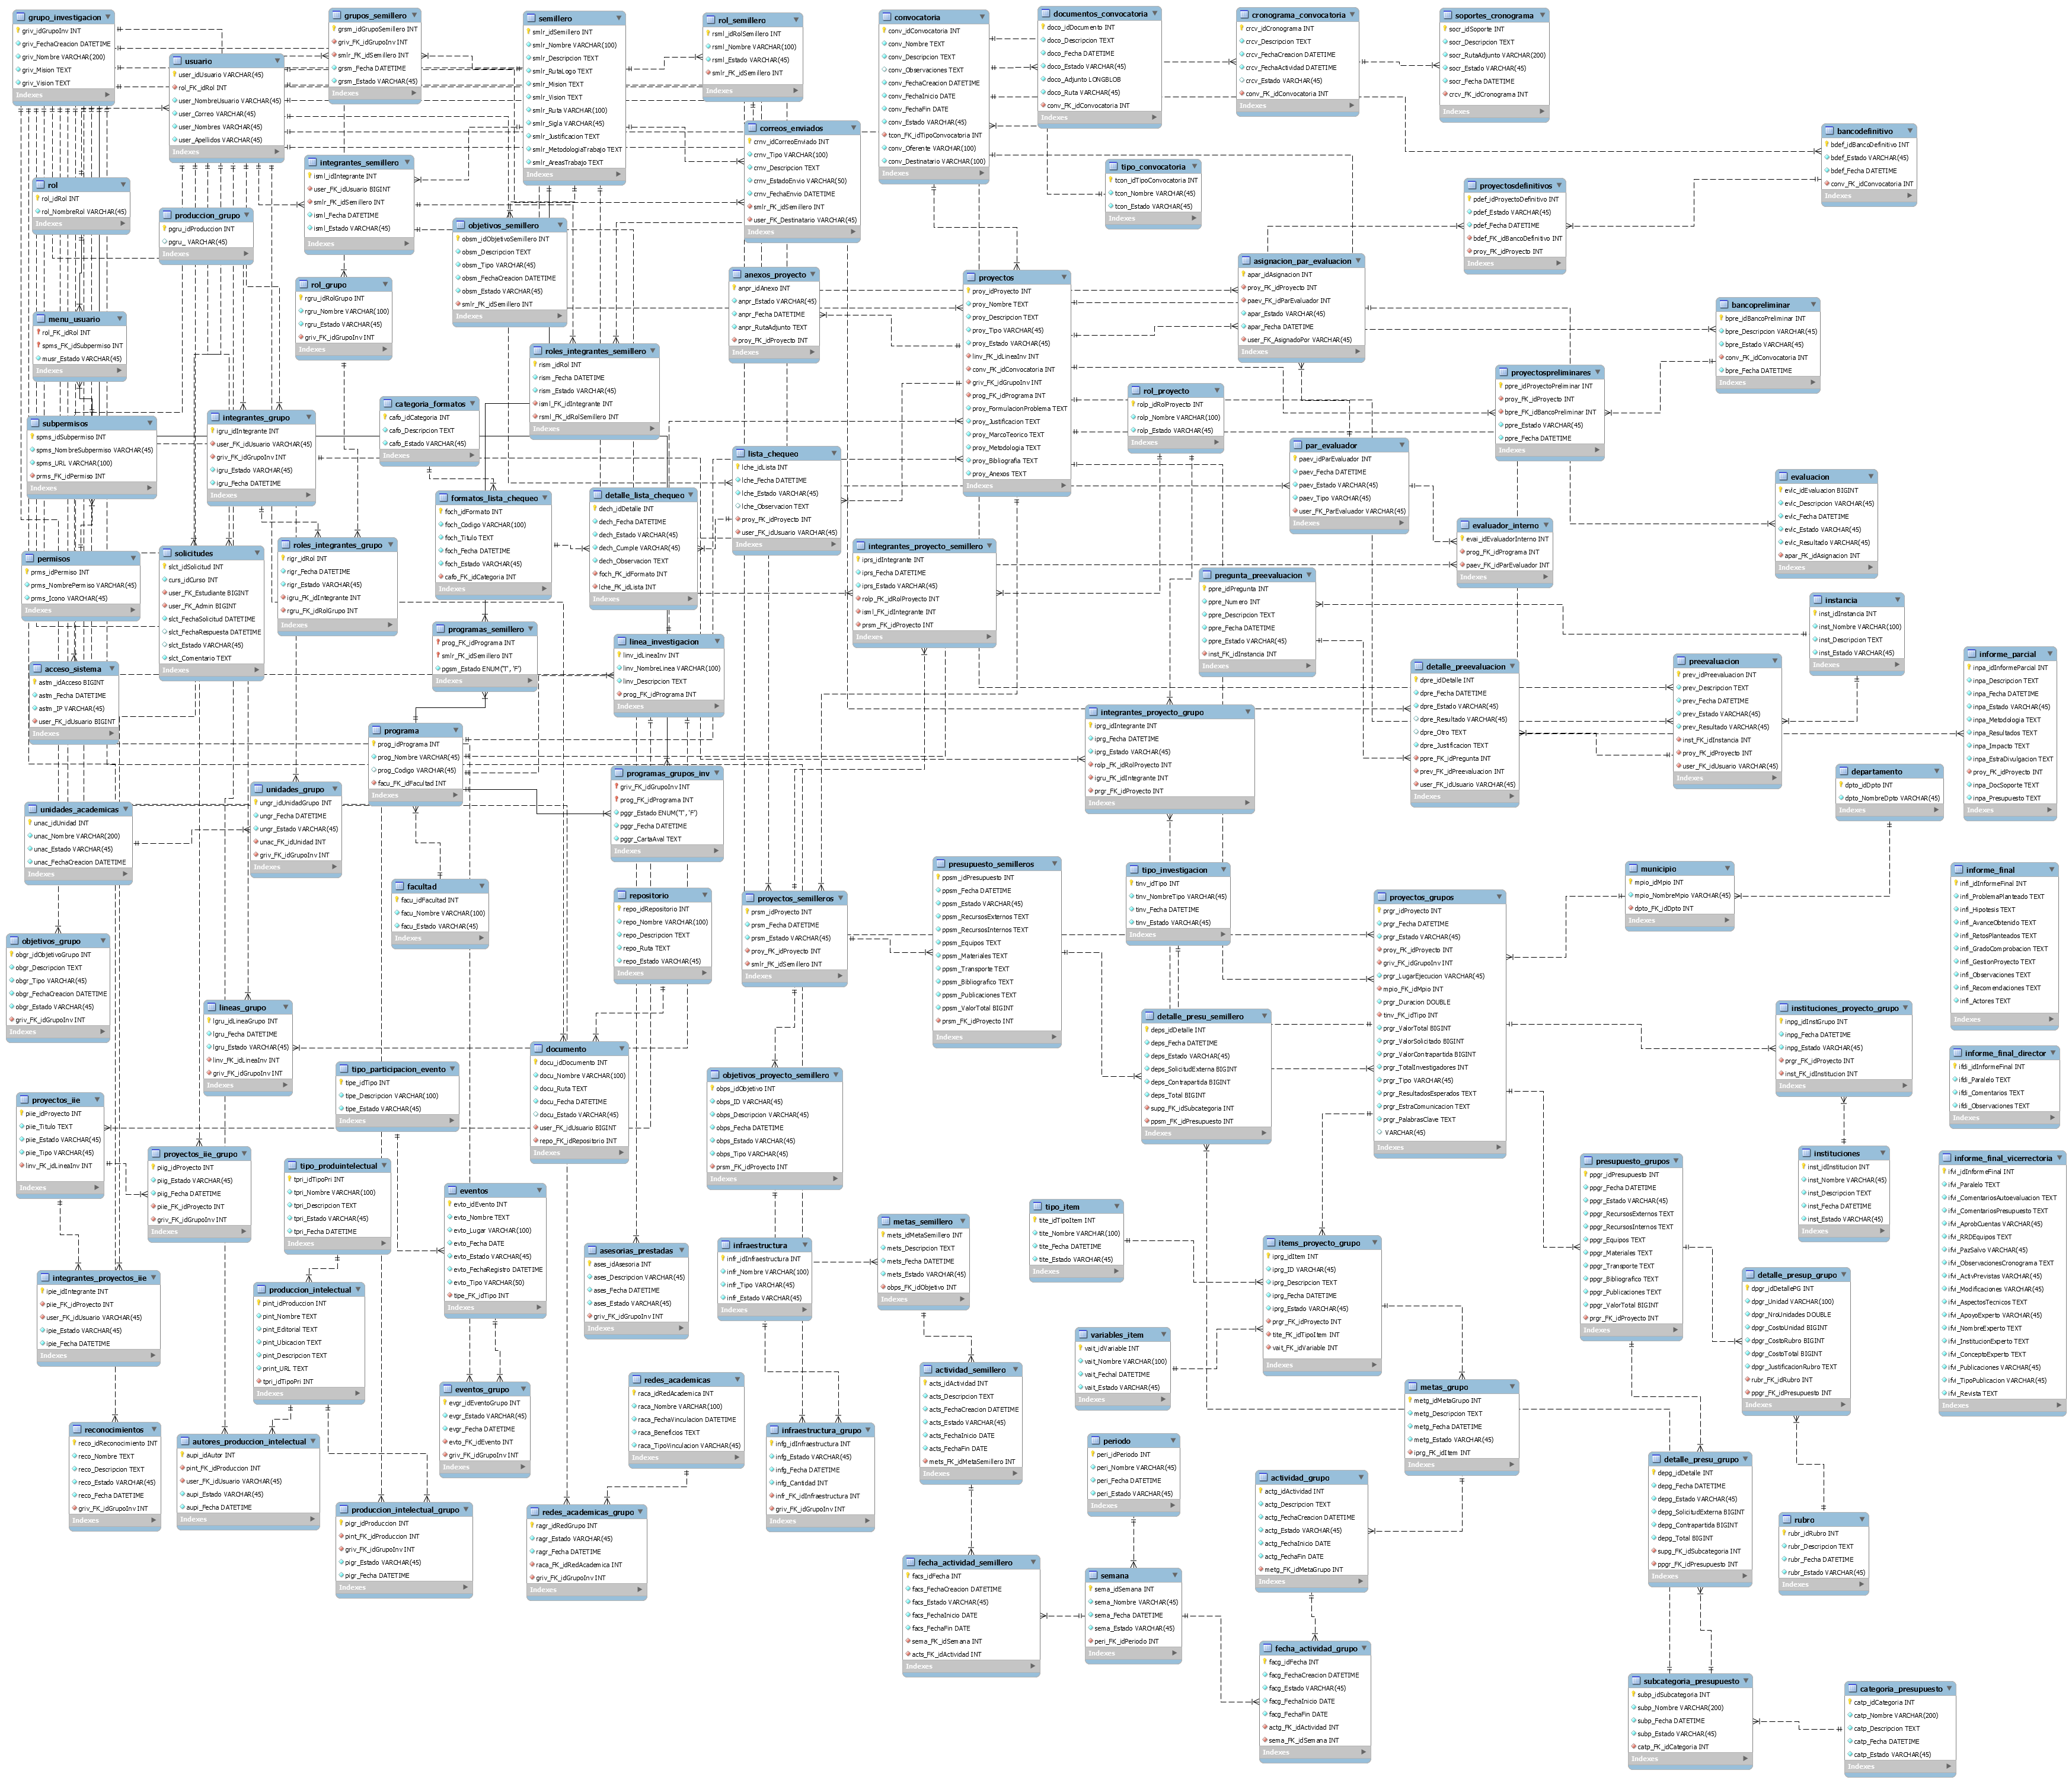
\includegraphics[width=\textwidth]{resources/modelo_relacional.PNG} %
\captionof{figure}{Modelo relacional base de datos}
\label{modelo_relacional_bd}

\section{Diccionario de datos}

A continuaci�n, se muestran la descripci�n (atributos, tipos y detalles) de las tablas usadas en el dise�o del sistema de informaci�n SIGEPI.

\begin{table}[ht]
	\caption{Tabla de diccionario - Usuario}
	\label{labelTableUsuario}
	\begin{tabularx}{\linewidth}{|X|X|X|X|X|X|}
		\hline
		\textbf{Nombre}	& \textbf{Tipo de dato} & \textbf{Permite Null} & \textbf{Primaria} & \textbf{For\'anea} & \textbf{Comentario} \\ \hline
		User Id Usuario & Cadena & Si & Si & No & Clave primaria \\ \hline
		Rol FK Id Rol	& Entero & Si & No & Si & Rol \\ \hline
		User Nombre Usuario & Cadena & Si & No & No & Nombre de usuario \\ \hline
		User Correo		& Cadena & Si & No & No & Correo electr�nico universidad \\ \hline
		User Nombres	& Cadena & Si & No & No & Nombres	\\ \hline
		User Apellidos	& Cadena & Si & No & No & Apellidos	\\ \hline
	\end{tabularx}
\end{table}

\begin{table}[ht]
	\caption{Tabla de diccionario - Semillero}
	\label{labelTableSemillero}
	\begin{tabularx}{\linewidth}{|X|l|X|X|X|X|}
		\hline
		\textbf{Nombre}	& \textbf{Tipo de dato} & \textbf{Permite Null} & \textbf{Primaria} & \textbf{For\'anea} & \textbf{Comentario} \\ \hline
		Smlr Id Semillero	& Entero & Si & Si & No & Id semillero \\ \hline 
		Smlr Nombre			& Cadena & Si & No & No & Nombre semillero \\ \hline 
		Smlr Descripcion 	& Texto largo & Si & No & No & Descripci�n \\ \hline 
		Smlr Ruta Logo 		& Texto largo & Si & No & No & URL Logo \\ \hline 
		Smlr Mision 		& Texto largo & Si & No & No & Misi�n \\ \hline 
		Smlr Vision 		& Texto largo & Si & No & No & Visi�n \\ \hline 
		Smlr Ruta 			& Cadena & Si & No & No & Ruta de semillero \\ \hline 
		Smlr Sigla 			& Cadena & Si & No & No & Siglas \\ \hline 
		Smlr Justificacion 	& Texto largo & Si & No & No & Justificaci�n \\ \hline 
		Smlr Metodologia Trabajo & Texto largo & Si & No & No & Metodolog�a \\ \hline 
		Smlr Areas Trabajo 	& Texto largo & Si & No & No & �reas de trabajos \\ \hline 	
	\end{tabularx}
\end{table}

\begin{table}[ht]
	\caption{Tabla de diccionario - Integrantes Semillero}
	\label{labelTableIntegrantesSemillero}
	\begin{tabularx}{\linewidth}{|X|l|X|X|X|X|}
		\hline
		\textbf{Nombre}	& \textbf{Tipo de dato} & \textbf{Permite Null} & \textbf{Primaria} & \textbf{For\'anea} & \textbf{Comentario} \\ \hline
		Isml Id Integrante	& Entero & Si & Si & No & Id integrante \\ \hline 
		User FK Id Usuario	& Entero & Si & No & Si & Id Usurario \\ \hline 
		Smlr FK Id Semillero& Entero & Si & No & Si & Id semillero \\ \hline 
		Isml Fecha			& Fecha  & Si & No & No & Fecha de registro \\ \hline 
		Isml Estado			& Cadena & Si & No & No & \\ \hline	
	\end{tabularx}
\end{table}

\begin{table}[ht]
	\caption{Tabla de diccionario - Rol}
	\label{labelTableRol}
	\begin{tabularx}{\linewidth}{|X|l|X|X|X|X|}
		\hline
		\textbf{Nombre}	& \textbf{Tipo de dato} & \textbf{Permite Null} & \textbf{Primaria} & \textbf{For\'anea} & \textbf{Comentario} \\ \hline
		Rol Id Rol		& Entero & Si & Si & No & \\ \hline 
		Rol Nombre Rol	& Cadena & Si & No & No & Nombre de rol \\ \hline	
	\end{tabularx}
\end{table}

\begin{table}[ht]
	\caption{Tabla de diccionario - Permisos}
	\label{labelTablePermisos}
	\begin{tabularx}{\linewidth}{|X|l|X|X|X|X|}
		\hline
		\textbf{Nombre}	& \textbf{Tipo de dato} & \textbf{Permite Null} & \textbf{Primaria} & \textbf{For\'anea} & \textbf{Comentario} \\ \hline
		Prms Id Permiso		& Entero & Si & Si & No &  \\ \hline 
		Prms Nombre Permiso & Cadena & Si & No & No & Nombre asignado al permiso \\ \hline 
		Prms Icono			& Cadena & Si & No & No & Referencia icono tipo CSS3 Boostrap \\ \hline 	
	\end{tabularx}
\end{table}


\begin{table}[ht]
	\caption{Tabla de diccionario - Subpermisos}
	\label{labelTableSubpermisos}
	\begin{tabularx}{\linewidth}{|X|l|X|X|X|X|}
		\hline
		\textbf{Nombre}	& \textbf{Tipo de dato} & \textbf{Permite Null} & \textbf{Primaria} & \textbf{For\'anea} & \textbf{Comentario} \\ \hline
		Spms Id Subpermiso		& Entero & Si & Si & No & \\ \hline 
		Spms Nombre Subpermiso	& Cadena & Si & No & No & \\ \hline 
		Spms URL				& Cadena & Si & No & No & URL asignado \\ \hline 
		Prms FK Id Permiso		& Entero & Si & No & Si & Relaci�n a permiso \\ \hline 	
	\end{tabularx}
\end{table}


\begin{table}[ht]
	\caption{Tabla de diccionario - Men\'u Usuario}
	\label{labelTableMenuUsuario}
	\begin{tabularx}{\linewidth}{|X|l|X|X|X|X|}
		\hline
		\textbf{Nombre}	& \textbf{Tipo de dato} & \textbf{Permite Null} & \textbf{Primaria} & \textbf{For\'anea} & \textbf{Comentario} \\ \hline
		RolFK Id Rol			& Entero & Si & Si & Si & \\ \hline 
		Spms FK Id Subpermiso	& Entero & Si & Si & Si & Relaci�n a subpermiso \\ \hline 
		Musr Estado				& Cadena & Si & No & No & Activo - Desactivado \\ \hline 	
	\end{tabularx}
\end{table}

\begin{table}[ht]
	\caption{Tabla de diccionario - Repositorio}
	\label{labelTableRepositorio}
	\begin{tabularx}{\linewidth}{|X|l|X|X|X|X|}
		\hline
		\textbf{Nombre}	& \textbf{Tipo de dato} & \textbf{Permite Null} & \textbf{Primaria} & \textbf{For\'anea} & \textbf{Comentario} \\ \hline
		Repo Id Repositorio & Entero & Si & Si & No & \\ \hline 
		Repo Nombre & Cadena & Si & No & No & Nombre de repositorio \\ \hline 
		Repo Descripcion & Texto largo & Si & No & No & \\ \hline 
		Repo Ruta & Texto largo & Si & No & No & Ruta del repositorio \\ \hline 
		Repo Estado & Cadena & Si & No & No & Activo - Desactivado \\ \hline 	
	\end{tabularx}
\end{table}


\begin{table}[ht]
	\caption{Tabla de diccionario - Documento}
	\label{labelTableDocumento}
	\begin{tabularx}{\linewidth}{|X|l|X|X|X|X|}
		\hline
		\textbf{Nombre}	& \textbf{Tipo de dato} & \textbf{Permite Null} & \textbf{Primaria} & \textbf{For\'anea} & \textbf{Comentario} \\ \hline
		DocuId Documento & Entero & Si & Si & No & \\ \hline 
		Docu Nombre & Cadena & Si & No & No & Nombre del documento \\ \hline 
		Docu Ruta & Texto largo & Si & No & No & Ruta del documento \\ \hline 
		Docu Fecha & Fecha & Si & No & No & Registro \\ \hline 
		Docu Estado & Cadena & No & No & No & \\ \hline 
		User FK Id Usuario & Entero & Si & No & Si & Relaci�n a usuario/ \\ \hline 
		Repo FK Id Repositorio & Entero & Si & No & Si & Relaci�n a repositorio / referencia contenedor de documentos \\ \hline 	
	\end{tabularx}
\end{table}

\begin{table}[ht]
	\caption{Tabla de diccionario - Correos Enviados}
	\label{labelTableCorreosEnviados}
	\begin{tabularx}{\linewidth}{|X|l|X|X|X|X|}
		\hline
		\textbf{Nombre}	& \textbf{Tipo de dato} & \textbf{Permite Null} & \textbf{Primaria} & \textbf{For\'anea} & \textbf{Comentario} \\ \hline
		Crnv Id Correo Enviado & Entero & Si & Si & No & \\ \hline 
		Crnv Tipo & Cadena & Si & No & No & Tipo de correo \\ \hline 
		Crnv Descripcion & Texto largo & Si & No & No & Descripci�n del correo \\ \hline 
		Crnv Estado Envio & Texto & Si & No & No & Activo - Desactivado \\ \hline 
		Crnv Fecha Envio & Fecha & Si & No & No & Fecha en que se envi� el correo \\ \hline 
		Smlr FK Id Semillero & Entero & Si & No & Si & Relaci�n a semillero / Semillero asignado \\ \hline 
		User FK Destinatario & Cadena & Si & No & Si & Usuario destinatario \\ \hline 	
	\end{tabularx}
\end{table}


\begin{table}[ht]
	\caption{Tabla de diccionario - Acceso Sistema}
	\label{labelTableAccesoSistema}
	\begin{tabularx}{\linewidth}{|X|l|X|X|X|X|}
		\hline
		\textbf{Nombre}	& \textbf{Tipo de dato} & \textbf{Permite Null} & \textbf{Primaria} & \textbf{For\'anea} & \textbf{Comentario} \\ \hline
		Astm Id Acceso & BI Entero & Si & Si & No & \\ \hline 
		Astm Fecha & Fecha & Si & No & No & Fecha de registro / ultimo acceso \\ \hline 
		Astm IP & Cadena & Si & No & No & Direcci�n IP del cliente \\ \hline 
		User FK Id Usuario & BI Entero & Si & No & Si & \\ \hline 	
	\end{tabularx}
\end{table}


\begin{table}[ht]
	\caption{Tabla de diccionario - Solicitudes}
	\label{labelTableSolicitudes}
	\begin{tabularx}{\linewidth}{|X|l|X|X|X|X|}
		\hline
		\textbf{Nombre}	& \textbf{Tipo de dato} & \textbf{Permite Null} & \textbf{Primaria} & \textbf{For\'anea} & \textbf{Comentario} \\ \hline
		Slct Id Solicitud & Entero & Si & Si & No & \\ \hline 
		Curs Id Curso & Entero & Si & No & No & \\ \hline 
		User FK Estudiante & BI Entero & Si & No & Si & Estudiante asignado \\ \hline 
		User FK Admin & Entero & Si & No & Si & \\ \hline 
		Slct Fecha Solicitud & Fecha & Si & No & No & \\ \hline 
		Slct Fecha Respuesta & Fecha & No & No & No & \\ \hline 
		Slct Estado & Cadena & No & No & No & Activo - Desactivado \\ \hline 
		Slct Comentario & Texto largo & Si & No & No & \\ \hline 	
	\end{tabularx}
\end{table}


\begin{table}[ht]
	\caption{Tabla de diccionario - Grupo Investigaci\'on}
	\label{labelTableGrupoInvestigacion}
	\begin{tabularx}{\linewidth}{|X|l|X|X|X|X|}
		\hline
		\textbf{Nombre}	& \textbf{Tipo de dato} & \textbf{Permite Null} & \textbf{Primaria} & \textbf{For\'anea} & \textbf{Comentario} \\ \hline
		Griv Id GrupoInv & Entero & Si & Si & No & \\ \hline 
		Griv Fecha Creacion & Fecha & Si & No & No & \\ \hline 
		Griv Nombre & Cadena & Si & No & No & Nombre del grupo de investigaci�n \\ \hline 
		Griv Mision & Texto largo & Si & No & No & \\ \hline 
		Griv Vision & Texto largo & Si & No & No & \\ \hline 	
	\end{tabularx}
\end{table}


\begin{table}[ht]
	\caption{Tabla de diccionario - Programa}
	\label{labelTablePrograma}
	\begin{tabularx}{\linewidth}{|X|l|X|X|X|X|}
		\hline
		\textbf{Nombre}	& \textbf{Tipo de dato} & \textbf{Permite Null} & \textbf{Primaria} & \textbf{For\'anea} & \textbf{Comentario} \\ \hline
		Prog Id Programa & Entero & Si & Si & No & \\ \hline 
		Prog Nombre & Cadena & Si & No & No & Nombre del programa \\ \hline 
		Prog Codigo & Cadena & No & No & No & C�digo del programa \\ \hline 
		Facu FK Id Facultad & Entero & Si & No & Si & \\ \hline 	
	\end{tabularx}
\end{table}


\begin{table}[ht]
	\caption{Tabla de diccionario - Programas Semillero}
	\label{labelTableProgramasSemillero}
	\begin{tabularx}{\linewidth}{|X|l|X|X|X|X|}
		\hline
		\textbf{Nombre}	& \textbf{Tipo de dato} & \textbf{Permite Null} & \textbf{Primaria} & \textbf{For\'anea} & \textbf{Comentario} \\ \hline
		Prog FK Id Programa & Entero & Si & Si & Si & \\ \hline 
		Smlr FK Id Semillero & Entero & Si & Si & Si & Semillero relacionado al programa \\ \hline 
		Pgsm Estado & Enumerable & Si & No & No & Activo - Desactivado \\ \hline 	
	\end{tabularx}
\end{table}


\begin{table}[ht]
	\caption{Tabla de diccionario - Programas Grupos Inv}
	\label{labelTableProgramasGruposInv}
	\begin{tabularx}{\linewidth}{|X|l|X|X|X|X|}
		\hline
		\textbf{Nombre}	& \textbf{Tipo de dato} & \textbf{Permite Null} & \textbf{Primaria} & \textbf{For\'anea} & \textbf{Comentario} \\ \hline
		Griv FKIdGrupoInv & Entero & Si & Si & Si & \\ \hline 
		Prog FKIdPrograma & Entero & Si & Si & Si & \\ \hline 
		Pggr Estado & ENUM('T', 'F') & Si & No & No & \\ \hline 
		Pggr Fecha & Fecha & Si & No & No & \\ \hline 
		Pggr CartaAval & Texto largo & Si & No & No & Contenido de carta aval\\ \hline 	
	\end{tabularx}
\end{table}


\begin{table}[ht]
	\caption{Tabla de diccionario - Proyectos}
	\label{labelTableProyectos}
	\begin{tabularx}{\linewidth}{|X|l|X|X|X|X|}
		\hline
		\textbf{Nombre}	& \textbf{Tipo de dato} & \textbf{Permite Null} & \textbf{Primaria} & \textbf{For\'anea} & \textbf{Comentario} \\ \hline
		Proy IdProyecto & Entero & Si & Si & No & \\ \hline 
		Proy Nombre & Texto largo & Si & No & No & \\ \hline 
		Proy Descripcion & Texto largo & Si & No & No & \\ \hline 
		Proy Tipo & Cadena & Si & No & No & \\ \hline 
		Pro Sitado & Cadena & Si & No & No & \\ \hline 
		Linv FKIdLineaInv & Entero & Si & No & Si & \\ \hline 
		Conv FKIdConvocatoria & Entero & Si & No & Si & \\ \hline 
		Griv FKIdGrupoInv & Entero & Si & No & Si & \\ \hline 
		Prog FKIdPrograma & Entero & Si & No & Si & \\ \hline 
		Proy FormulacionProblema & Texto largo & Si & No & No & \\ \hline 
		Proy Justificacion & Texto largo & Si & No & No & \\ \hline 
		Proy MarcoTeorico & Texto largo & Si & No & No & \\ \hline 
		Proy Metodologia & Texto largo & Si & No & No & \\ \hline 
		Proy Bibliografia & Texto largo & Si & No & No & \\ \hline 
		Proy Anexos & Texto largo & Si & No & No & \\ \hline 	
	\end{tabularx}
\end{table}


\begin{table}[ht]
	\caption{Tabla de diccionario - Rol Semillero}
	\label{labelTableRolSemillero}
	\begin{tabularx}{\linewidth}{|X|l|X|X|X|X|}
		\hline
		\textbf{Nombre}	& \textbf{Tipo de dato} & \textbf{Permite Null} & \textbf{Primaria} & \textbf{For\'anea} & \textbf{Comentario} \\ \hline
		Rsml IdRolSemillero & Entero & Si & Si & No & \\ \hline 
		Rsml Nombre & Cadena & Si & No & No & \\ \hline 
		Rsml Estado & Cadena & Si & No & No & \\ \hline 
		Smlr FKIdSemillero & Entero & Si & No & Si & \\ \hline 	
	\end{tabularx}
\end{table}


\begin{table}[ht]
	\caption{Tabla de diccionario - Par Evaluador}
	\label{labelTableParEvaluador}
	\begin{tabularx}{\linewidth}{|X|l|X|X|X|X|}
		\hline
		\textbf{Nombre}	& \textbf{Tipo de dato} & \textbf{Permite Null} & \textbf{Primaria} & \textbf{For\'anea} & \textbf{Comentario} \\ \hline
		Paev IdParEvaluador & Entero & Si & Si & No & \\ \hline 
		Paev Fecha & Fecha & Si & No & No & \\ \hline 
		Paev Estado & Cadena & Si & No & No & \\ \hline 
		Paev Tipo & Cadena & Si & No & No & \\ \hline 
		User FKParEvaluador & Cadena & Si & No & Si & \\ \hline 	
	\end{tabularx}
\end{table}


\begin{table}[ht]
	\caption{Tabla de diccionario - Actividad Semillero}
	\label{labelTableActividadSemillero}
	\begin{tabularx}{\linewidth}{|X|l|X|X|X|X|}
		\hline
		\textbf{Nombre}	& \textbf{Tipo de dato} & \textbf{Permite Null} & \textbf{Primaria} & \textbf{For\'anea} & \textbf{Comentario} \\ \hline
		Acts IdActividad & Entero & Si & Si & No & \\ \hline 
		Acts Descripcion & Texto largo & Si & No & No & \\ \hline 
		Acts FechaCreacion & Fecha & Si & No & No & \\ \hline 
		Acts Estado & Cadena & Si & No & No & \\ \hline 
		Acts FechaInicio & DATE & Si & No & No & \\ \hline 
		Acts FechaFin & DATE & Si & No & No & \\ \hline 
		Mets FKIdMetaSemillero & Entero & Si & No & Si & \\ \hline 	
	\end{tabularx}
\end{table}


\begin{table}[ht]
	\caption{Tabla de diccionario - Convocatoria}
	\label{labelTableConvocatoria}
	\begin{tabularx}{\linewidth}{|X|l|X|X|X|X|}
		\hline
		\textbf{Nombre}	& \textbf{Tipo de dato} & \textbf{Permite Null} & \textbf{Primaria} & \textbf{For\'anea} & \textbf{Comentario} \\ \hline
		Conv IdConvocatoria & Entero & Si & Si & No & \\ \hline 
		Conv Nombre & Texto largo & Si & No & No & \\ \hline 
		Conv Descripcion & Texto largo & Si & No & No & \\ \hline 
		Conv Observaciones & Texto largo & No & No & No & \\ \hline 
		Conv FechaCreacion & Fecha & Si & No & No & \\ \hline 
		Conv FechaInicio & DATE & Si & No & No & \\ \hline 
		Conv FechaFin & DATE & Si & No & No & \\ \hline 
		Conv Estado & Cadena & Si & No & No & \\ \hline 
		Tcon FKIdTipoConvocatoria & Entero & Si & No & Si & \\ \hline 
		Conv Oferente & Cadena & Si & No & No & \\ \hline 
		Conv Destinatario & Cadena & Si & No & No & \\ \hline 	
	\end{tabularx}
\end{table}


\begin{table}[ht]
	\caption{Tabla de diccionario - Banco Preliminar}
	\label{labelTableBancopreliminar}
	\begin{tabularx}{\linewidth}{|X|l|X|X|X|X|}
		\hline
		\textbf{Nombre}	& \textbf{Tipo de dato} & \textbf{Permite Null} & \textbf{Primaria} & \textbf{For\'anea} & \textbf{Comentario} \\ \hline
		Bpre IdBancoPreliminar & Entero & Si & Si & No & \\ \hline 
		Bpre Descripcion & Cadena & Si & No & No & \\ \hline 
		Bpre Estado & Cadena & Si & No & No & \\ \hline 
		Conv FKIdConvocatoria & Entero & Si & No & Si & \\ \hline 
		Bpre Fecha & Fecha & Si & No & No & \\ \hline 	
	\end{tabularx}
\end{table}


\begin{table}[ht]
	\caption{Tabla de diccionario - Proyectos preliminares}
	\label{labelTableProyectospreliminares}
	\begin{tabularx}{\linewidth}{|X|l|X|X|X|X|}
		\hline
		\textbf{Nombre}	& \textbf{Tipo de dato} & \textbf{Permite Null} & \textbf{Primaria} & \textbf{For\'anea} & \textbf{Comentario} \\ \hline
		Ppre IdProyectoPreliminar & Entero & Si & Si & No & \\ \hline 
		Proy FKIdProyecto & Entero & Si & No & Si & \\ \hline 
		Bpre FKIdBancoPreliminar & Entero & Si & No & Si & \\ \hline 
		Ppre Estado & Cadena & Si & No & No & \\ \hline 
		Ppre Fecha & Fecha & Si & No & No & \\ \hline 	
	\end{tabularx}
\end{table}


\begin{table}[ht]
	\caption{Tabla de diccionario - Banco definitivo}
	\label{labelTableBancodefinitivo}
	\begin{tabularx}{\linewidth}{|X|l|X|X|X|X|}
		\hline
		\textbf{Nombre}	& \textbf{Tipo de dato} & \textbf{Permite Null} & \textbf{Primaria} & \textbf{For\'anea} & \textbf{Comentario} \\ \hline
		Bdef IdBancoDefinitivo & Entero & Si & Si & No & \\ \hline 
		Bdef Estado & Cadena & Si & No & No & \\ \hline 
		Bdef Fecha & Fecha & Si & No & No & \\ \hline 
		Conv FKIdConvocatoria & Entero & Si & No & Si & \\ \hline 	
	\end{tabularx}
\end{table}


\begin{table}[ht]
	\caption{Tabla de diccionario - Proyectos definitivos}
	\label{labelTableProyectosdefinitivos}
	\begin{tabularx}{\linewidth}{|X|l|X|X|X|X|}
		\hline
		\textbf{Nombre}	& \textbf{Tipo de dato} & \textbf{Permite Null} & \textbf{Primaria} & \textbf{For\'anea} & \textbf{Comentario} \\ \hline
		Pdef IdProyectoDefinitivo & Entero & Si & Si & No & \\ \hline 
		Pdef Estado & Cadena & Si & No & No & \\ \hline 
		Pdef Fecha & Fecha & Si & No & No & \\ \hline 
		Bdef FKIdBancoDefinitivo & Entero & Si & No & Si & \\ \hline 
		Proy FKIdProyecto & Entero & Si & No & Si & \\ \hline 	
	\end{tabularx}
\end{table}


\begin{table}[ht]
	\caption{Tabla de diccionario - Evaluaci\'on}
	\label{labelTableEvaluacion}
	\begin{tabularx}{\linewidth}{|X|l|X|X|X|X|}
		\hline
		\textbf{Nombre}	& \textbf{Tipo de dato} & \textbf{Permite Null} & \textbf{Primaria} & \textbf{For\'anea} & \textbf{Comentario} \\ \hline
		Evlc IdEvaluacion & BI Entero & Si & Si & No & \\ \hline 
		Evlc Descripcion & Cadena & Si & No & No & \\ \hline 
		Evlc Fecha & Fecha & Si & No & No & \\ \hline 
		Evlc Estado & Cadena & Si & No & No & \\ \hline 
		Evlc Resultado & Cadena & Si & No & No & \\ \hline 
		Apar FKIdAsignacion & Entero & Si & No & Si & \\ \hline 	
	\end{tabularx}
\end{table}


\begin{table}[ht]
	\caption{Tabla de diccionario - Tipo Convocatoria}
	\label{labelTableTipoConvocatoria}
	\begin{tabularx}{\linewidth}{|X|l|X|X|X|X|}
		\hline
		\textbf{Nombre}	& \textbf{Tipo de dato} & \textbf{Permite Null} & \textbf{Primaria} & \textbf{For\'anea} & \textbf{Comentario} \\ \hline
		Tcon IdTipoConvocatoria & Entero & Si & Si & No & \\ \hline 
		Tcon Nombre & Cadena & Si & No & No & \\ \hline 
		Tcon Estado & Cadena & Si & No & No & \\ \hline 	
	\end{tabularx}
\end{table}


\begin{table}[ht]
	\caption{Tabla de diccionario - Linea Investigaci\'on}
	\label{labelTableLineaInvestigacion}
	\begin{tabularx}{\linewidth}{|X|l|X|X|X|X|}
		\hline
		\textbf{Nombre}	& \textbf{Tipo de dato} & \textbf{Permite Null} & \textbf{Primaria} & \textbf{For\'anea} & \textbf{Comentario} \\ \hline
		Linv IdLineaInv & Entero & Si & Si & No & \\ \hline 
		Linv NombreLinea & Cadena & Si & No & No & \\ \hline 
		Linv Descripcion & Texto largo & Si & No & No & \\ \hline 
		Prog FKIdPrograma & Entero & Si & No & Si & \\ \hline 	
	\end{tabularx}
\end{table}


\begin{table}[ht]
	\caption{Tabla de diccionario - Facultad}
	\label{labelTableFacultad}
	\begin{tabularx}{\linewidth}{|X|l|X|X|X|X|}
		\hline
		\textbf{Nombre}	& \textbf{Tipo de dato} & \textbf{Permite Null} & \textbf{Primaria} & \textbf{For\'anea} & \textbf{Comentario} \\ \hline
		Facu IdFacultad & Entero & Si & Si & No & \\ \hline 
		Facu Nombre & Cadena & Si & No & No & \\ \hline 
		Facu Estado & Cadena & Si & No & No & \\ \hline 	
	\end{tabularx}
\end{table}


\begin{table}[ht]
	\caption{Tabla de diccionario - Evaluador Interno}
	\label{labelTableEvaluadorInterno}
	\begin{tabularx}{\linewidth}{|X|l|X|X|X|X|}
		\hline
		\textbf{Nombre}	& \textbf{Tipo de dato} & \textbf{Permite Null} & \textbf{Primaria} & \textbf{For\'anea} & \textbf{Comentario} \\ \hline
		Evai IdEvaluadorInterno & Entero & Si & Si & No & \\ \hline 
		Prog FKIdPrograma & Entero & Si & No & Si & \\ \hline 
		Paev FKIdParEvaluador & Entero & Si & No & Si & \\ \hline 	
	\end{tabularx}
\end{table}


\begin{table}[ht]
	\caption{Tabla de diccionario - Asignaci\'on Par Evaluaci\'on}
	\label{labelTableAsignacionParEvaluacion}
	\begin{tabularx}{\linewidth}{|X|l|X|X|X|X|}
		\hline
		\textbf{Nombre}	& \textbf{Tipo de dato} & \textbf{Permite Null} & \textbf{Primaria} & \textbf{For\'anea} & \textbf{Comentario} \\ \hline
		Apar IdAsignacion & Entero & Si & Si & No & \\ \hline 
		Proy FKIdProyecto & Entero & Si & No & Si & \\ \hline 
		Paev FKIdParEvaluador & Entero & Si & No & Si & \\ \hline 
		Apar Estado & Cadena & Si & No & No & \\ \hline 
		Apar Fecha & Fecha & Si & No & No & \\ \hline 
		User FKAsignadoPor & Cadena & Si & No & Si & \\ \hline 	
	\end{tabularx}
\end{table}


\begin{table}[ht]
	\caption{Tabla de diccionario - Preevaluacion}
	\label{labelTablePreevaluacion}
	\begin{tabularx}{\linewidth}{|X|l|X|X|X|X|}
		\hline
		\textbf{Nombre}	& \textbf{Tipo de dato} & \textbf{Permite Null} & \textbf{Primaria} & \textbf{For\'anea} & \textbf{Comentario} \\ \hline
		Prev IdPreevaluacion & Entero & Si & Si & No & \\ \hline 
		Prev Descripcion & Texto largo & Si & No & No & \\ \hline 
		Prev Fecha & Fecha & Si & No & No & \\ \hline 
		Prev Estado & Cadena & Si & No & No & \\ \hline 
		Prev Resultado & Cadena & Si & No & No & \\ \hline 
		Inst FKIdInstancia & Entero & Si & No & Si & \\ \hline 
		Proy FKIdProyecto & Entero & Si & No & Si & \\ \hline 
		User FKIdUsuario & Cadena & Si & No & Si & \\ \hline 	
	\end{tabularx}
\end{table}


\begin{table}[ht]
	\caption{Tabla de diccionario - Instancia}
	\label{labelTableInstancia}
	\begin{tabularx}{\linewidth}{|X|l|X|X|X|X|}
		\hline
		\textbf{Nombre}	& \textbf{Tipo de dato} & \textbf{Permite Null} & \textbf{Primaria} & \textbf{For\'anea} & \textbf{Comentario} \\ \hline
		Inst IdInstancia & Entero & Si & Si & No & \\ \hline 
		Inst Nombre & Cadena & Si & No & No & \\ \hline 
		Inst Descripcion & Texto largo & Si & No & No & \\ \hline 
		Inst Estado & Cadena & Si & No & No & \\ \hline 	
	\end{tabularx}
\end{table}


\begin{table}[ht]
	\caption{Tabla de diccionario - Integrantes Grupo}
	\label{labelTableIntegrantesGrupo}
	\begin{tabularx}{\linewidth}{|X|l|X|X|X|X|}
		\hline
		\textbf{Nombre}	& \textbf{Tipo de dato} & \textbf{Permite Null} & \textbf{Primaria} & \textbf{For\'anea} & \textbf{Comentario} \\ \hline
		Igru IdIntegrante & Entero & Si & Si & No & \\ \hline 
		User FKIdUsuario & Cadena & Si & No & Si & \\ \hline 
		Griv FKIdGrupoInv & Entero & Si & No & Si & \\ \hline 
		Igru Estado & Cadena & Si & No & No & \\ \hline 
		Igru Fecha & Fecha & Si & No & No & \\ \hline 	
	\end{tabularx}
\end{table}


\begin{table}[ht]
	\caption{Tabla de diccionario - Proyectos Semilleros}
	\label{labelTableProyectosSemilleros}
	\begin{tabularx}{\linewidth}{|X|l|X|X|X|X|}
		\hline
		\textbf{Nombre}	& \textbf{Tipo de dato} & \textbf{Permite Null} & \textbf{Primaria} & \textbf{For\'anea} & \textbf{Comentario} \\ \hline
		Prsm IdProyecto & Entero & Si & Si & No & \\ \hline 
		Prsm Fecha & Fecha & Si & No & No & \\ \hline 
		Prsm Estado & Cadena & Si & No & No & \\ \hline 
		Proy FKIdProyecto & Entero & Si & No & Si & \\ \hline 
		Smlr FKIdSemillero & Entero & Si & No & Si & \\ \hline 	
	\end{tabularx}
\end{table}


\begin{table}[ht]
	\caption{Tabla de diccionario - Proyectos Grupos}
	\label{labelTableProyectosGrupos}
	\begin{tabularx}{\linewidth}{|X|l|X|X|X|X|}
		\hline
		\textbf{Nombre}	& \textbf{Tipo de dato} & \textbf{Permite Null} & \textbf{Primaria} & \textbf{For\'anea} & \textbf{Comentario} \\ \hline
		Prgr IdProyecto & Entero & Si & Si & No & \\ \hline 
		Prgr Fecha & Fecha & Si & No & No & \\ \hline 
		Prgr Estado & Cadena & Si & No & No & \\ \hline 
		Proy FKIdProyecto & Entero & Si & No & Si & \\ \hline 
		Griv FKIdGrupoInv & Entero & Si & No & Si & \\ \hline 
		Prgr LugarEjecucion & Cadena & Si & No & No & \\ \hline 
		Mpio FKIdMpio & Entero & Si & No & Si & \\ \hline 
		Prgr Duracion & DOUBLE & Si & No & No & \\ \hline 
		Tinv FKIdTipo & Entero & Si & No & Si & \\ \hline 
		Prgr ValorTotal & BI Entero & Si & No & No & \\ \hline 
		Prgr ValorSolicitado & BI Entero & Si & No & No & \\ \hline 
		Prgr ValorContrapartida & BI Entero & Si & No & No & \\ \hline 
		Prgr TotalInvestigadores & Entero & Si & No & No & \\ \hline 
		Prgr Tipo & Cadena & Si & No & No & \\ \hline 
		Prgr ResultadosEsperados & Texto largo & Si & No & No & \\ \hline 
		Prgr EstraComunicacion & Texto largo & Si & No & No & \\ \hline 
		Prgr PalabrasClave & Texto largo & Si & No & No & \\ \hline 
		& Cadena & No & No & No & \\ \hline 	
	\end{tabularx}
\end{table}


\begin{table}[ht]
	\caption{Tabla de diccionario - Roles Integrantes Semillero}
	\label{labelTableRolesIntegrantesSemillero}
	\begin{tabularx}{\linewidth}{|X|l|X|X|X|X|}
		\hline
		\textbf{Nombre}	& \textbf{Tipo de dato} & \textbf{Permite Null} & \textbf{Primaria} & \textbf{For\'anea} & \textbf{Comentario} \\ \hline
		Rism IdRol & Entero & Si & Si & No & \\ \hline 
		Rism Fecha & Fecha & Si & No & No & \\ \hline 
		Rism Estado & Cadena & Si & No & No & \\ \hline 
		Isml FKIdIntegrante & Entero & Si & No & Si & \\ \hline 
		Rsml FKIdRolSemillero & Entero & Si & No & Si & \\ \hline 	
	\end{tabularx}
\end{table}


\begin{table}[ht]
	\caption{Tabla de diccionario - Rol Grupo}
	\label{labelTableRolGrupo}
	\begin{tabularx}{\linewidth}{|X|l|X|X|X|X|}
		\hline
		\textbf{Nombre}	& \textbf{Tipo de dato} & \textbf{Permite Null} & \textbf{Primaria} & \textbf{For\'anea} & \textbf{Comentario} \\ \hline
		Rgru IdRolGrupo & Entero & Si & Si & No & \\ \hline 
		Rgru Nombre & Cadena & Si & No & No & \\ \hline 
		Rgru Estado & Cadena & Si & No & No & \\ \hline 
		Griv FKIdGrupoInv & Entero & Si & No & Si & \\ \hline 	
	\end{tabularx}
\end{table}


\begin{table}[ht]
	\caption{Tabla de diccionario - Roles Integrantes Grupo}
	\label{labelTableRolesIntegrantesGrupo}
	\begin{tabularx}{\linewidth}{|X|l|X|X|X|X|}
		\hline
		\textbf{Nombre}	& \textbf{Tipo de dato} & \textbf{Permite Null} & \textbf{Primaria} & \textbf{For\'anea} & \textbf{Comentario} \\ \hline
		Rigr IdRol & Entero & Si & Si & No & \\ \hline 
		Rigr Fecha & Fecha & Si & No & No & \\ \hline 
		Rigr Estado & Cadena & Si & No & No & \\ \hline 
		Igru FKIdIntegrante & Entero & Si & No & Si  & \\ \hline 
		Rgru FKIdRolGrupo & Entero & Si & No & Si & \\ \hline 	
	\end{tabularx}
\end{table}


\begin{table}[ht]
	\caption{Tabla de diccionario - Objetivos Proyecto Semillero}
	\label{labelTableObjetivosProyectoSemillero}
	\begin{tabularx}{\linewidth}{|X|l|X|X|X|X|}
		\hline
		\textbf{Nombre}	& \textbf{Tipo de dato} & \textbf{Permite Null} & \textbf{Primaria} & \textbf{For\'anea} & \textbf{Comentario} \\ \hline
		Obps IdObjetivo & Entero & Si & Si & No & \\ \hline 
		Obps ID & Cadena & Si & No & No & \\ \hline 
		Obps Descripcion & Cadena & Si & No & No & \\ \hline 
		Obps Fecha & Fecha & Si & No & No & \\ \hline 
		Obps Estado & Cadena & Si & No & No & \\ \hline 
		Obps Tipo & Cadena & Si & No & No & \\ \hline 
		Prsm FKIdProyecto & Entero & Si & No & Si & \\ \hline 	
	\end{tabularx}
\end{table}


\begin{table}[ht]
	\caption{Tabla de diccionario - Informe Parcial}
	\label{labelTableInformeParcial}
	\begin{tabularx}{\linewidth}{|X|l|X|X|X|X|}
		\hline
		\textbf{Nombre}	& \textbf{Tipo de dato} & \textbf{Permite Null} & \textbf{Primaria} & \textbf{For\'anea} & \textbf{Comentario} \\ \hline
		Inpa IdInformeParcial & Entero & Si & Si & No & \\ \hline 
		Inpa Descripcion & Texto largo & Si & No & No & \\ \hline 
		Inpa Fecha & Fecha & Si & No & No & \\ \hline 
		Inpa Estado & Cadena & Si & No & No & \\ \hline 
		Inpa Metodologia & Texto largo & Si & No & No & \\ \hline 
		Inpa Resultados & Texto largo & Si & No & No & \\ \hline 
		Inpa Impacto & Texto largo & Si & No & No & \\ \hline 
		Inpa EstraDivulgacion & Texto largo & Si & No & No & \\ \hline 
		Proy FKIdProyecto & Entero & Si & No & Si & \\ \hline 
		Inpa DocSoporte & Texto largo & Si & No & No & \\ \hline 
		Inpa Presupuesto & Texto largo & Si & No & No & \\ \hline 	
	\end{tabularx}
\end{table}


\begin{table}[ht]
	\caption{Tabla de diccionario - Integrantes Proyecto Semillero}
	\label{labelTableIntegrantesProyectoSemillero}
	\begin{tabularx}{\linewidth}{|X|l|X|X|X|X|}
		\hline
		\textbf{Nombre}	& \textbf{Tipo de dato} & \textbf{Permite Null} & \textbf{Primaria} & \textbf{For\'anea} & \textbf{Comentario} \\ \hline
		Iprs Id Integrante & Entero & Si & Si & No & \\ \hline 
		Iprs Fecha	& Fecha		& Si 	 & No & No & \\ \hline 
		Iprs Estado & Cadena	& Si	 & No & No & \\ \hline 
		Rolp FK IdRolProyecto	& Entero & Si & No & Si & \\ \hline 
		Isml FK IdIntegrante	& Entero & Si & No & Si & \\ \hline 
		Prsm FK IdProyecto		& Entero & Si & No & Si & \\ \hline 	
	\end{tabularx}
\end{table}


\begin{table}[ht]
	\caption{Tabla de diccionario - Rol Proyecto}
	\label{labelTableRolProyecto}
	\begin{tabularx}{\linewidth}{|X|l|X|X|X|X|}
		\hline
		\textbf{Nombre}	& \textbf{Tipo de dato} & \textbf{Permite Null} & \textbf{Primaria} & \textbf{For\'anea} & \textbf{Comentario} \\ \hline
		Rolp Id Rol Proyecto & Entero & Si & Si & No & \\ \hline 
		Rolp Nombre & Cadena & Si & No & No & \\ \hline 
		Rolp Estado & Cadena & Si & No & No & \\ \hline 	
	\end{tabularx}
\end{table}


\begin{table}[ht]
	\caption{Tabla de diccionario - Informe Final}
	\label{labelTableInformeFinal}
	\begin{tabularx}{\linewidth}{|X|l|X|X|X|X|}
		\hline
		\textbf{Nombre}	& \textbf{Tipo de dato} & \textbf{Permite Null} & \textbf{Primaria} & \textbf{For\'anea} & \textbf{Comentario} \\ \hline
		Infi Id Informe Final & Entero & Si & Si & No & \\ \hline 
		Infi Problema Planteado & Texto largo & Si & No & No & \\ \hline 
		Infi Hipotesis & Texto largo & Si & No & No & \\ \hline 
		Infi Avance Obtenido & Texto largo & Si & No & No & \\ \hline 
		Infi Retos Planteados & Texto largo & Si & No & No & \\ \hline 
		Infi Grado Comprobacion & Texto largo & Si & No & No & \\ \hline 
		Infi Gestion Proyecto & Texto largo & Si & No & No & \\ \hline 
		Infi Observaciones & Texto largo & Si & No & No & \\ \hline 
		Infi Recomendaciones & Texto largo & Si & No & No & \\ \hline 
		Infi Actores & Texto largo & Si & No & No & \\ \hline 	
	\end{tabularx}
\end{table}


\begin{table}[ht]
	\caption{Tabla de diccionario - Informe Final}
	\label{labelTableInformeFinal}
	\begin{tabularx}{\linewidth}{|X|l|X|X|X|X|}
		\hline
		\textbf{Nombre}	& \textbf{Tipo de dato} & \textbf{Permite Null} & \textbf{Primaria} & \textbf{For\'anea} & \textbf{Comentario} \\ \hline
		Infi Id Informe Final & Entero & Si & Si & No & \\ \hline 
		Infi Problema Planteado & Texto largo & Si & No & No & Describe el problema del informe \\ \hline 
		Infi Hipotesis & Texto largo & Si & No & No & Hip�tesis del informe \\ \hline 
		Infi Avance Obtenido & Texto largo & Si & No & No & \\ \hline 
		Infi Retos Planteados & Texto largo & Si & No & No & \\ \hline 
		Infi Grado Comprobacion & Texto largo & Si & No & No & \\ \hline 
		Infi Gestion Proyecto & Texto largo & Si & No & No & \\ \hline 
		Infi Observaciones & Texto largo & Si & No & No & \\ \hline 
		Infi Recomendaciones & Texto largo & Si & No & No & \\ \hline 
		Infi Actores & Texto largo & Si & No & No & \\ \hline 	
	\end{tabularx}
\end{table}


\begin{table}[ht]
	\caption{Tabla de diccionario - Cronograma Convocatoria}
	\label{labelTableCronogramaConvocatoria}
	\begin{tabularx}{\linewidth}{|X|l|X|X|X|X|}
		\hline
		\textbf{Nombre}	& \textbf{Tipo de dato} & \textbf{Permite Null} & \textbf{Primaria} & \textbf{For\'anea} & \textbf{Comentario} \\ \hline
		Crcv Id Cronograma & Entero & Si & Si & No & \\ \hline 
		Crcv Descripcion & Texto largo & Si & No & No & \\ \hline 
		Crcv Fecha Creacion & Fecha & Si & No & No & \\ \hline 
		Crcv Fecha Actividad & Fecha & Si & No & No & Fecha propuesta para actividad\\ \hline 
		Crcv Estado & Cadena & No & No & No & Activo - Desactivado \\ \hline 
		Conv FK Id Convocatoria & Entero & Si & No & Si & \\ \hline 	
	\end{tabularx}
\end{table}

\begin{table}[ht]
	\caption{Tabla de diccionario - Soportes Cronograma}
	\label{labelTableSoportesCronograma}
	\begin{tabularx}{\linewidth}{|X|l|X|X|X|X|}
		\hline
		\textbf{Nombre}	& \textbf{Tipo de dato} & \textbf{Permite Null} & \textbf{Primaria} & \textbf{For\'anea} & \textbf{Comentario} \\ \hline
		Socr Id Soporte & Entero & Si & Si & No & \\ \hline 
		Socr Descripcion & Texto largo & Si & No & No & \\ \hline 
		Socr Ruta Adjunto & Cadena & Si & No & No & Ruta del soporte cronograma \\ \hline 
		Socr Estado & Cadena & Si & No & No & Activo - Desactivado \\ \hline 
		Socr Fecha & Fecha & Si & No & No & \\ \hline 
		Crcv FK Id Cronograma & Entero & Si & No & Si & Relaci�n a cronograma \\ \hline	
	\end{tabularx}
\end{table}

\begin{table}[ht]
	\caption{Tabla de diccionario - Producci\'on Grupo}
	\label{labelTableProduccionGrupo}
	\begin{tabularx}{\linewidth}{|l|X|X|X|X|X|}
		\hline
		\textbf{Nombre}	& \textbf{Tipo de dato} & \textbf{Permite Null} & \textbf{Primaria} & \textbf{For\'anea} & \textbf{Comentario} \\ \hline
		Pgru Id Produccion & Entero & Si & Si & No & Clave primaria \\ \hline 
		Pgru & Cadena & No & No & No & Producci�n grupo \\ \hline 	
	\end{tabularx}
\end{table}

\begin{table}[ht]
	\caption{Tabla de diccionario - Unidades Acad\'emicas}
	\label{labelTableUnidadesAcademicas}
	\begin{tabularx}{\linewidth}{|X|l|X|X|X|X|}
		\hline
		\textbf{Nombre}	& \textbf{Tipo de dato} & \textbf{Permite Null} & \textbf{Primaria} & \textbf{For\'anea} & \textbf{Comentario} \\ \hline
		Unac Id Unidad	& Entero & Si & Si & No & \\ \hline 
		Unac Nombre		& Cadena & Si & No & No & \\ \hline 
		Unac Estado		& Cadena & Si & No & No & Activo - Desactivado\\ \hline 
		Unac Fecha Creacion & Fecha & Si & No & No & \\ \hline	
	\end{tabularx}
\end{table}
	\chapter{Licitaci\'on de requisitos}

\section{Objetivos del sistem\'a}

\begin{table}[H]
	\centering
	\caption{Requisito - Gestionar convocatoria}
	\label{label_req_gconv}
	\begin{tabular}{|l|p{13cm}|}
		\hline
		OBJ-001 & \begin{tabular}[c]{@{}l@{}}
			Gestionar convocatorias
		\end{tabular} \\ \hline
		Versi\'on & 002 (2016-08-03) \\ \hline
		Autores & \begin{tabular}[c]{@{}l@{}}
			Angie Zuleta Cardona (Universidad de la Amazonia) \\
			Derly Viviana  Murcia Serrano (Universidad de la Amazonia)\\
			Mateo Ceballos Bermudez (Universidad de la Amazonia) \\
			Nicol Dayana Endo Ruiz (Universidad de la Amazonia)
		\end{tabular} \\ \hline
		Fuentes & \begin{tabular}[c]{@{}l@{}}
			Alberto Fajardo Oliveros (Uniamazonia) \\
			Dora Lida Suarez Castro (Uniamazonia)
		\end{tabular} \\ \hline
		Descripci\'on & \begin{tabular}[c]{@{}l@{}}
			El sistema deber\'a gestionar la informaci\'on \\ 
			respecto a las distintas convocatorias en el \\ 
			marco de semilleros y grupos de investigaci\'on.
		\end{tabular} \\ \hline
		SubObjetivos & \\ \hline
		Importancia & Vital \\ \hline
		Urgencia & Inmediatamente \\ \hline
		Estado & En Construcci\'on \\ \hline
		Estabilidad & Alta \\ \hline
		Comentarios & Ninguno \\ \hline
	\end{tabular}
\end{table}


\begin{table}[H]
	\centering
	\caption{Requisito - Gestionar propuestas de proyectos}
	\label{label_req_gpdp}
	\begin{tabular}{|l|l|}
		\hline
		OBJ-002      & \begin{tabular}[c]{@{}l@{}}
			Gestionar propuestas de proyectos
		\end{tabular} \\ \hline
		Versi\'on    & 003 (2016-08-03) \\ \hline
		Autores      & \begin{tabular}[c]{@{}l@{}}
			Angie Zuleta Cardona (Universidad de la Amazonia)\\
			Derly Viviana  Murcia Serrano (Universidad de la Amazonia) \\ 
			Mateo Ceballos Bermudez (Universidad de la Amazonia) \\ 
			Nicol Dayana Endo Ruiz (Universidad de la Amazonia)
		\end{tabular} \\ \hline
		Fuentes      & \begin{tabular}[c]{@{}l@{}}
			Alberto Fajardo Oliveros (Uniamazonia) \\
			Dora Lida Suarez Castro (Uniamazonia)
		\end{tabular} \\ \hline
		Descripci\'on  & \begin{tabular}[c]{@{}l@{}}
			El sistema debe gestionar la informaci\'on que\\
			respecta a cada una de las propuestas que se \\
			presentan, sin importar el origen de estas.
		\end{tabular} \\  \hline
		SubObjetivos & \\  \hline
		Importancia  & Vital  \\ \hline
		Urgencia     & Inmediatamente \\
		Estado       & En Construcci\'on \\
		Estabilidad  & Alta \\ \hline
		Comentarios  & Ninguno \\  \hline
	\end{tabular}
\end{table}

\begin{table}[H]
	\centering
	\caption{Requisito - Gesti\'on de informaci\'on proyectos de investigaci\'on}
	\label{label_req_gipi}
	\begin{tabular}{|l|l|}
		\hline
		Autores      & \begin{tabular}[c]{@{}l@{}}
			Angie Zuleta Cardona (Universidad de la Amazonia)\\
			Derly Viviana  Murcia Serrano (Universidad de la Amazonia)\\
			Mateo Ceballos Bermudez (Universidad de la Amazonia)\\
			Nicol Dayana Endo Ruiz (Universidad de la Amazonia)
		\end{tabular} \\ \hline
		Fuentes      & \begin{tabular}[c]{@{}l@{}}
			Alberto Fajardo Oliveros (Uniamazonia) \\
			Dora Lida Suarez Castro (Uniamazonia)
		\end{tabular} \\ \hline
		Descripci\'on  & \begin{tabular}[c]{@{}l@{}}
			El sistema permitir\'a gestionar la informaci\'on\\
			correspondiente a cada proyecto de investigaci\'on
		\end{tabular} \\ \hline
		SubObjetivos & \\ \hline
		Importancia  & Vital \\ \hline
		Urgencia     & Inmediatamente \\ \hline
		Estado       & En Construcci\'on \\ \hline
		Estabilidad  & Alta \\ \hline
		Comentarios & \\ \hline
	\end{tabular}
\end{table}


\begin{table}[H]
	\centering
	\caption{Requisito - Gestionar informaci\'on de Grupos de Investigaci\'on}
	\label{label_req_gigi}
	\begin{tabular}{|l|l|}
		\hline
		OBJ-004      & \begin{tabular}[c]{@{}l@{}}
			Gestionar informaci\'on de Grupos de Investigaci\'on
		\end{tabular} \\ \hline
		Versi\'on    & 001 (2016-08-03) \\ \hline
		Autores      & \begin{tabular}[c]{@{}l@{}}
			Angie Zuleta Cardona (Universidad de la Amazonia)\\   
			Derly Viviana  Murcia Serrano (Universidad de la Amazonia)\\
			Mateo Ceballos Bermudez (Universidad de la Amazonia)\\
			Nicol Dayana Endo Ruiz (Universidad de la Amazonia)
		\end{tabular} \\ \hline
		Fuentes      & \begin{tabular}[c]{@{}l@{}}
			Alberto Fajardo Oliveros (Uniamazonia)\\
			Dora Lida Suarez Castro (Uniamazonia)
		\end{tabular} \\ \hline
		Descripci\'on & \begin{tabular}[c]{@{}l@{}}
			El sistema deber\'a suministrar la informaci\'on\\
			respecto a cada uno de los grupos de Investigaci\'on
		\end{tabular} \\ \hline
		SubObjetivos & \\ \hline
		Importancia  & Vital \\ \hline
		Urgencia     & Inmediatamente \\ \hline
		Estado       & En Construcci\'on \\ \hline
		Estabilidad  & Alta \\ \hline
		Comentarios  & \\ \hline
	\end{tabular}
\end{table}


\begin{table}[H]
	\centering
	\caption{Requisito - Gestionar informaci\'on de semilleros de investigaci\'on}
	\label{label_req_gisi}
	\begin{tabular}{|l|l|}
		\hline
		OBJ-005      & \begin{tabular}[c]{@{}l@{}}
			Gestionar informaci\'on de semilleros de investigaci\'on
		\end{tabular} \\ \hline
		Versi\'on    & 001 (2016-08-03) \\ \hline
		Autores      & \begin{tabular}[c]{@{}l@{}}
			Angie Zuleta Cardona (Universidad de la Amazonia)\\
			Derly Viviana  Murcia Serrano (Universidad de la Amazonia) \\ 
			Mateo Ceballos Bermudez (Universidad de la Amazonia)\\ 
			Nicol Dayana Endo Ruiz (Universidad de la Amazonia)
		\end{tabular} \\ \hline
		Fuentes      & \begin{tabular}[c]{@{}l@{}}
			Alberto Fajardo Oliveros (Uniamazonia) \\
			Dora Lida Suarez Castro (Uniamazonia)  \\
		\end{tabular} \\ \hline
		Descripci\'on & \begin{tabular}[c]{@{}l@{}}
			El sistema deber\'a permitir la gesti\'on de la\\
			informaci\'on que corresponde a los semilleros de \\ investigaci\'on.
		\end{tabular} \\  \hline
		SubObjetivos & \\ \hline
		Importancia  & Vital \\ \hline
		Urgencia     & Inmediatamente \\ \hline
		Estado       & En Construcci\'on \\ \hline
		Estabilidad  & Alta \\ \hline
		Comentarios  & Ninguno. \\ \hline
	\end{tabular}
\end{table}

\begin{table}[H]
	\centering
	\caption{Requisito - Gestionar investigador}
	\label{label_req_ginv}
	\begin{tabular}{|l|l|}
		\hline
		OBJ-007      & Gestionar investigador \\ \hline
		Versi\'on    & 002 (2016-08-03) \\ \hline
		Autores      & \begin{tabular}[c]{@{}l@{}}
			Angie Zuleta Cardona (Universidad de la Amazonia)\\   
			Derly Viviana  Murcia Serrano (Universidad de la Amazonia)\\
			Mateo Ceballos Bermudez (Universidad de la Amazonia)\\
			Nicol Dayana Endo Ruiz (Universidad de la Amazonia)
		\end{tabular} \\ \hline
		Fuentes      & \begin{tabular}[c]{@{}l@{}}
			Alberto Fajardo Oliveros (Uniamazonia)\\
			Dora Lida Suarez Castro (Uniamazonia)
		\end{tabular} \\ \hline
		Descripci\'on  & \begin{tabular}[c]{@{}l@{}}
			El sistema deber\'a permitir la gesti\'on de la\\   
			informaci\'on que respecta a los investigadores.
		\end{tabular} \\ \hline
		SubObjetivos & \\ \hline
		Importancia  & Vital \\ \hline
		Urgencia     & Inmediatamente \\ \hline
		Estado       & En Construcci\'on \\ \hline
		Estabilidad  & Alta \\ \hline
		Comentarios  & Ninguna. \\ \hline
	\end{tabular}
\end{table}

\begin{table}[H]
	\centering
	\caption{Requisito - Gestionar par}
	\label{label_req_gpar}
	\begin{tabular}{|l|l|}
		\hline
		OBJ-008      & Gestionar par \\ \hline
		Versi\'on    & 001 (2016-09-09) \\ \hline
		Autores      & \begin{tabular}[c]{@{}l@{}}
			Angie Zuleta Cardona (Universidad de la Amazonia)\\
			Derly Viviana  Murcia Serrano (Universidad de la Amazonia)\\
			Nicol Dayana Endo Ruiz (Universidad de la Amazonia)
		\end{tabular} \\ \hline
		Fuentes      & \begin{tabular}[c]{@{}l@{}}
			Alberto Fajardo Oliveros (Uniamazonia) \\
			Dora Lida Suarez Castro (Uniamazonia)
		\end{tabular} \\ \hline
		Descripcion  & \begin{tabular}[c]{@{}l@{}}
			El sistema deber\'a permitir la gesti\'on de la \\
			informaci\'on referente a los pares evaluadores.
		\end{tabular} \\ \hline
		SubObjetivos & \\ \hline
		Importancia  & Vital \\ \hline
		Urgencia     & Inmediatamente \\ \hline
		Estado       & En Construcci\'on \\ \hline
		Estabilidad  & Alta \\ \hline
		Comentarios  & Ninguno \\ \hline
	\end{tabular}
\end{table}

\begin{table}[H]
	\centering
	\caption{Requisito - Gestionar evaluaci\'on}
	\label{label_req_ge}
	\begin{tabular}{|l|l|}
		\hline
		OBJ-009      & Gestionar evaluaci\'on \\ \hline
		Versi\'on    & 001 (2016-09-09) \\ \hline
		Autores      & \begin{tabular}[c]{@{}l@{}}
			Angie Zuleta Cardona (Universidad de la Amazonia)\\
			Derly Viviana  Murcia Serrano (Universidad de la Amazonia) \\
			Nicol Dayana Endo Ruiz (Universidad de la Amazonia)
		\end{tabular} \\ \hline
		Fuentes      & \begin{tabular}[c]{@{}l@{}}
			Alberto Fajardo Oliveros (Uniamazonia) \\
			Dora Lida Suarez Castro (Uniamazonia)
		\end{tabular} \\ \hline
		Descripci\'on  & \begin{tabular}[c]{@{}l@{}}
			El sistema permitir\'a gestionar la informaci\'on\\
			referente a la evaluaci\'on de las propuestas de \\
			investigaci\'on por parte de los pares evaluadores.
		\end{tabular}\\ \hline
		SubObjetivos & \begin{tabular}[c]{@{}l@{}}
			OBJ-008 Gestionar par
		\end{tabular} \\ \hline
		Importancia  & Vital \\ \hline
		Urgencia     & Inmediatamente \\ \hline
		Estado       & En Construcci\'on \\ \hline
		Estabilidad  & Alta \\ \hline
		Comentarios  & Ninguno \\  \hline
	\end{tabular}
\end{table}

\begin{table}[H]
	\centering
	\caption{Requisito - Gestionar Banco de Elegibles}
	\label{label_req_gbde}
	\begin{tabular}{|l|l|}
		\hline
		OBJ-010      & \begin{tabular}[c]{@{}l@{}}
			Gestionar Banco de Elegibles
		\end{tabular} \\ \hline
		Versi\'on      & 001 (2016-09-09) \\ \hline
		Autores      & \begin{tabular}[c]{@{}l@{}}
			Angie Zuleta Cardona (Universidad de la Amazonia)\\
			Derly Viviana  Murcia Serrano (Universidad de la Amazonia)\\
			Nicol Dayana Endo Ruiz (Universidad de la Amazonia)
		\end{tabular} \\ \hline
		Fuentes      & \begin{tabular}[c]{@{}l@{}}
			Alberto Fajardo Oliveros (Uniamazonia) \\
			Dora Lida Suarez Castro (Uniamazonia)
		\end{tabular} \\ \hline
		Descripci\'on  & \begin{tabular}[c]{@{}l@{}}
			El Sistema deber\'a permitir a los usuarios la\\   gesti\'on del banco de elegibles de propuestas de investigaci\'on, \\
			sea un banco\\   de elegible preliminar o definitivo.
		\end{tabular}        \\ \hline
		SubObjetivos & \begin{tabular}[c]{@{}l@{}}
			OBJ-009 - Gestionar evaluaci\'on
		\end{tabular} \\ \hline
		Importancia  & Vital \\ \hline
		Urgencia     & Inmediatamente \\ \hline
		Estado       & En Construcci\'on \\ \hline
		Estabilidad  & Alta \\ \hline
		Comentarios  & Ninguno. \\ \hline
	\end{tabular}
\end{table}

\begin{table}[H]
	\centering
	\caption{Requisito - Gestionar Preevaluaciones}
	\label{label_req_gp}
	\begin{tabular}{|l|l|}
		\hline
		OBJ-011      & Gestionar Preevaluaciones \\ \hline
		Versi\'on    & 002 (2016-09-09) \\ \hline
		Autores      & \begin{tabular}[c]{@{}l@{}}
			Angie Zuleta Cardona (Universidad de la Amazonia)\\   Derly Viviana  Murcia Serrano\\   (Universidad de la Amazonia) Nicol Dayana Endo Ruiz (Universidad de la\\   Amazonia)
		\end{tabular} \\ \hline
		Fuentes      & \begin{tabular}[c]{@{}l@{}}
			Alberto Fajardo Oliveros (Uniamazonia) \\   
			Dora Lida Suarez Castro (Uniamazonia)
		\end{tabular} \\ \hline
		Descripci\'on  & \begin{tabular}[c]{@{}l@{}}
			El sistema deber\'a permitir la gesti\'on de la informaci\'on\\   referente a las pre- evaluaciones de las propuestas de investigaci\'on
		\end{tabular} \\ \hline
		SubObjetivos & \begin{tabular}[c]{@{}l@{}}
			OBJ-002 - Gestionar propuestas de proyectos
		\end{tabular} \\ \hline
		Importancia  & Vital \\ \hline
		Urgencia     & Inmediatamente \\ \hline
		Estado       & En Construcci\'on \\ \hline
		Estabilidad  & Alta \\ \hline
		Comentarios  & Ninguno \\  \hline
	\end{tabular}
\end{table}

\begin{table}[H]
	\centering
	\caption{Requisito - Gestionar l\'ineas de investigaci\'on}
	\label{label_req_gli}
	\begin{tabular}{|l|l|}
		\hline
		OBJ-012      & \begin{tabular}[c]{@{}l@{}}
			Gestionar L\'ineas de Investigaci\'on
		\end{tabular} \\ \hline
		Versi\'on    & 001 (2016-09-09) \\ \hline
		Autores      & \begin{tabular}[c]{@{}l@{}}
			Angie Zuleta Cardona (Universidad de la Amazonia)\\
			Derly Viviana  Murcia Serrano (Universidad de la Amazonia)\\
			Nicol Dayana Endo Ruiz (Universidad de la Amazonia)
		\end{tabular} \\ \hline
		Fuentes      & \begin{tabular}[c]{@{}l@{}}
			Alberto Fajardo Oliveros (Uniamazonia) \\  
			Dora Lida Suarez Castro (Uniamazonia)
		\end{tabular} \\ \hline
		Descripci\'on & \begin{tabular}[c]{@{}l@{}}
			El Sistema deber\'a permitir la gesti\'on de la\\   informaci\'on que corresponde a las l\'ineas de investigaci\'on relacionadas con\\   los proyectos de investigaci\'on.
		\end{tabular} \\ \hline
		SubObjetivos & \\ \hline
		Importancia  & Vital \\ \hline
		Urgencia     & Inmediatamente \\ \hline
		Estado       & En Construcci\'on  \\ \hline
		Estabilidad  & Alta \\ \hline
		Comentarios  & Ninguno.\\ \hline
	\end{tabular}
\end{table}

\begin{table}[H]
	\centering
	\caption{Requisito - Gestionar inscripci\'on}
	\label{label_req_gins}
	\begin{tabular}{|l|l|}
		\hline
		OBJ-012      & Gestionar inscripci\'on \\ \hline
		Versi\'on    & 001 (2016-09-09) \\ \hline
		Autores      & \begin{tabular}[c]{@{}l@{}}
			Angie Zuleta Cardona (Universidad de la Amazonia)\\ 
			Derly Viviana  Murcia Serrano (Universidad de la Amazonia) \\   
			Nicol Dayana Endo Ruiz (Universidad de la Amazonia)
		\end{tabular} \\ \hline
		Fuentes      & \begin{tabular}[c]{@{}l@{}}
			Alberto Fajardo Oliveros (Uniamazonia) \\
			Dora Lida Suarez Castro (Uniamazonia)
		\end{tabular} \\ \hline
		Descripci\'on & \begin{tabular}[c]{@{}l@{}}
			El Sistema deber\'a permitir la gesti\'on de la\\
			informaci\'on respecto a las distintas inscripciones para propuestas de\\   iniciativa docente en el marco de semilleros y grupos de investigaci\'on
		\end{tabular} \\ \hline
		SubObjetivos & \\ \hline
		Importancia  & Vital \\ \hline
		Urgencia     & Inmediatamente \\ \hline
		Estado       & En Construcci\'on \\ \hline
		Estabilidad  & Alta \\ \hline
		Comentarios  & Ninguno. \\ \hline
	\end{tabular}
\end{table}


\section{Actores del sistema}

\begin{table}[H]
	\centering
	\caption{Actor - Administrador}
	\label{label_actor_admin}
	\begin{tabular}{|l|l|}
		\hline
		ACT-001     & Administrador \\ \hline
		Versi\'on   & 003 (2016-08-04) \\ \hline
		Autores     & \begin{tabular}[c]{@{}l@{}}
			Angie Zuleta Cardona (Universidad de la Amazonia)\\
			Derly Viviana  Murcia Serrano (Universidad de la Amazonia)\\
			Mateo Ceballos Bermudez (Universidad de la Amazonia)\\
			Nicol Dayana Endo Ruiz (Universidad de la Amazonia)
		\end{tabular} \\ \hline
		Fuentes     & \begin{tabular}[c]{@{}l@{}}
			Alberto Fajardo Oliveros (Uniamazonia)\\
			Dora Lida Suarez Castro (Uniamazonia)
		\end{tabular} \\ \hline
		Descripci\'on & \begin{tabular}[c]{@{}l@{}}
			Este actor representa el administrador general\\   del sistema
		\end{tabular} \\ \hline
		Comentarios & Ninguno \\ \hline
	\end{tabular}
\end{table}

\begin{table}[H]
	\centering
	\caption{Actor - Vicerrector}
	\label{label_actor_vice}
	\begin{tabular}{|l|l|}
		\hline
		ACT-002     & Vicerrector \\ \hline
		Versi\'on   & 003 (2016-08-04) \\ \hline
		Autores     & \begin{tabular}[c]{@{}l@{}}
			Angie Zuleta Cardona (Universidad de la Amazonia)\\   
			Derly Viviana  Murcia Serrano (Universidad de la Amazonia)\\
			Mateo Ceballos Bermudez (Universidad de la Amazonia)\\
			Nicol Dayana Endo Ruiz (Universidad de la Amazonia)
		\end{tabular} \\ \hline
		Fuentes     & \begin{tabular}[c]{@{}l@{}}
			Alberto Fajardo Oliveros (Uniamazonia) \\
			Dora Lida Suarez Castro (Uniamazonia)
		\end{tabular}
		\\ \hline
		Descripci\'on & \begin{tabular}[c]{@{}l@{}}
			Este actor representa el vicerrector de\\   investigaciones.\end{tabular} \\ \hline
		Comentarios & Ninguno \\ \hline
	\end{tabular}
\end{table}

\begin{table}[]
	\centering
	\caption{Actor - Auxiliar de investigaci\'on}
	\label{label_actor_auxin}
	\begin{tabular}{|l|l|}
		\hline
		ACT-003     & \begin{tabular}[c]{@{}l@{}}
			Auxiliar de investigaci\'on
		\end{tabular} \\ \hline
		Versi\'on     & 003 (2016-08-04) \\ \hline
		Autores     & \begin{tabular}[c]{@{}l@{}}
			Angie Zuleta Cardona (Universidad de la Amazonia)\\
			Derly Viviana  Murcia Serrano (Universidad de la Amazonia) \\
			Mateo Ceballos Bermudez (Universidad de la Amazonia) \\
			Nicol Dayana Endo Ruiz (Universidad de la Amazonia)
		\end{tabular} \\ \hline
		Fuentes     & \begin{tabular}[c]{@{}l@{}}
			Alberto Fajardo Oliveros (Uniamazonia) \\
			Dora Lida Suarez Castro (Uniamazonia)
		\end{tabular} \\ \hline
		Descripci\'on & \begin{tabular}[c]{@{}l@{}}
			Este actor representa el auxiliar de \\ 
			investigaci\'on que har\'a uso del sistema.
		\end{tabular} \\ \hline
		Comentarios & Ninguno \\ \hline
	\end{tabular}
\end{table}

\begin{table}[H]
	\centering
	\caption{Actor - Investigador}
	\label{label_actor_inv}
	\begin{tabular}{|l|l|}
		\hline
		ACT-004     & Investigador \\ \hline
		Versi\'on   & 003 (2016-08-04) \\ \hline
		Autores     & \begin{tabular}[c]{@{}l@{}}
			Angie Zuleta Cardona (Universidad de la Amazonia)\\
			Derly Viviana  Murcia Serrano (Universidad de la Amazonia) \\
			Mateo Ceballos Bermudez (Universidad de la Amazonia) \\
			Nicol Dayana Endo Ruiz (Universidad de la Amazonia)
		\end{tabular} \\ \hline
		Fuentes     & \begin{tabular}[c]{@{}l@{}}
			Alberto Fajardo Oliveros (Uniamazonia) \\
			Dora Lida Suarez Castro (Uniamazonia)
		\end{tabular} \\ \hline
		Descripci\'on & \begin{tabular}[c]{@{}l@{}}
			Este actor representa el investigador de cada uno\\   de los proyectos de investigaci\'on.
		\end{tabular} \\ \hline
		Comentarios & Ninguno \\ \hline
	\end{tabular}
\end{table}

\begin{table}[]
	\centering
	\caption{Actor - Evaluador}
	\label{label_actor_eval}
	\begin{tabular}{|l|l|}
		\hline
		ACT-005     & Evaluador \\ \hline
		Versi\'on   & 003 (2016-08-04) \\ \hline
		Autores     & \begin{tabular}[c]{@{}l@{}}
			Angie Zuleta Cardona (Universidad de la Amazonia)\\
			Derly Viviana  Murcia Serrano (Universidad de la Amazonia)\\
			Mateo Ceballos Bermudez (Universidad de la Amazonia)\\
			Nicol Dayana Endo Ruiz (Universidad de la Amazonia)
		\end{tabular} \\ \hline
		Fuentes     & \begin{tabular}[c]{@{}l@{}}
			Alberto Fajardo Oliveros (Uniamazonia)\\
			Dora Lida Suarez Castro (Uniamazonia)
		\end{tabular} \\ \hline
		Descripci\'on & \begin{tabular}[c]{@{}l@{}}
			Este actor representa los entes que hacen parte\\   
			del proceso de evaluaci\'on y preevaluaci\'on de las \\
			propuestas de investigaci\'on tanto de los grupos \\
			como de los semilleros. En este caso ser\'ia el Comit\'e de \\  
			investigaciones, Comit\'e de Curr\'iculo, Consejo de Facultad.
		\end{tabular} \\ \hline
		Comentarios & Ninguno \\ \hline
	\end{tabular}
\end{table}

\begin{table}[H]
	\centering
	\caption{Actor - Par evaluador}
	\label{label_actor_pare}
	\begin{tabular}{|l|l|}
		\hline
		ACT-006     & Par evaluador \\ \hline
		Versi\'on     & 003 (2016-08-04) \\ \hline
		Autores     & \begin{tabular}[c]{@{}l@{}}
			Angie Zuleta Cardona (Universidad de la Amazonia)\\   Derly Viviana  Murcia Serrano\\   (Universidad de la Amazonia) Mateo Ceballos\\   Bermudez (Universidad de la Amazonia) Nicol Dayana Endo Ruiz (Universidad de\\   la Amazonia)\end{tabular} \\ \hline
		Fuentes     & \begin{tabular}[c]{@{}l@{}}Alberto \\   Fajardo Oliveros (Uniamazonia) Dora Lida Suarez Castro (Uniamazonia)\end{tabular}                                                                                                                                                     \\ \hline
		Descripci\'on & \begin{tabular}[c]{@{}l@{}}
			Este actor representa el evaluador de cada una de\\   las propuestas de investigaci\'on y de los informes finales de los proyectos.
		\end{tabular} \\ \hline
		Comentarios & Ninguno \\ \hline
	\end{tabular}
\end{table}


\section{Requisitos funcionales}

\begin{table}[H]
	\centering
	\caption{Requisito funcional - RF-001}
	\label{my-label}
	\resizebox{16cm}{!} {	
	\begin{tabular}{|l|l|}
		\hline
		RF-001 & \begin{tabular}[c]{@{}l@{}}
			Registrar convocatoria de propuestas para \\
			proyectos de Grupo de Investigaci\'on
		\end{tabular} \\ \hline
		Versi\'on & 007 (2016-08-04) \\ \hline
		Autores & \begin{tabular}[c]{@{}l@{}}
			Angie Zuleta Cardona (Universidad de la Amazonia)\\   
			Derly Viviana  Murcia Serrano (Universidad de la Amazonia)\\
			Mateo Ceballos Bermudez (Universidad de la Amazonia) \\
			Nicol Dayana Endo Ruiz (Universidad de la Amazonia)
		\end{tabular} \\ \hline
		Fuentes & \begin{tabular}[c]{@{}l@{}}
			Alberto Fajardo Oliveros (Uniamazonia) \\
			Dora Lida Suarez Castro (Uniamazonia)
		\end{tabular} \\ \hline
		Objetivos asociados & \begin{tabular}[c]{@{}l@{}}
			OBJ-001 - Gestionar convocatorias
		\end{tabular} \\ \hline
		Requisitos asociados & \begin{tabular}[c]{@{}l@{}}
			RF-006 \textless Registra propuesta de\\   proyecto\textgreater
		\end{tabular} \\ \hline
		Descripci\'on & \begin{tabular}[c]{@{}l@{}}
			El sistema deber\'a permitir al usuario en \\
			el rol Vicerrector (ACT-002) y Auxiliar de \\
			investigaci\'on (ACT-003) registrar la respectiva\\
			convocatoria  de propuestas de proyectos en \\
			el marco de los Grupos de Investigaci\'on.
		\end{tabular} \\ \hline
		Precondici\'on & \begin{tabular}[c]{@{}l@{}}
			El Usuario debe iniciar sesi\'on en el sistema\\   
			antes de llevar a cabo el proceso de registro.
		\end{tabular} \\ \hline
		Secuencia Normal & Paso \\
		1 & \begin{tabular}[c]{@{}l@{}}
			El Usuario En el rol de Vicerrector (ACT-002) y\\   
			Auxiliar  de investigaci\'on (ACT-003) solicita\\   
			al sistema, iniciar el proceso de registrar \\
			(publicar) la convocatoria.
		\end{tabular} \\
		2 & \begin{tabular}[c]{@{}l@{}}
			El sistema muestra el formulario para el registro\\   de convocatoria.
		\end{tabular} \\
		3 & \begin{tabular}[c]{@{}l@{}}
			El Usuario en el rol de Vicerrector (ACT-002) y\\
			Auxiliar  de investigaci\'on (ACT-003) registra\\   
			(publica) la convocatoria diligenciando el formato \\ 
			teniendo en cuenta los t\'erminos de referencia, que \\ 
			deben ser cumplidos.
		\end{tabular} \\
		4 & \begin{tabular}[c]{@{}l@{}}
			El sistema valida la informaci\'on respectiva de la\\   convocatoria.
		\end{tabular} \\
		5 & \begin{tabular}[c]{@{}l@{}}
			El sistema almacena la informaci\'on de la referida\\   convocatoria en la base de datos.
		\end{tabular} \\
		6 & \begin{tabular}[c]{@{}l@{}}
			El sistema env\'ia un mensaje de confirmaci\'on de\\   
			registro al usuario que est\'e efectuando la operaci\'on.
		\end{tabular} \\
		7 & \begin{tabular}[c]{@{}l@{}}
			El sistema una vez confirme el registro, enviar\'a\\
			una notificaci\'on al correo de los l\'ideres de todos\\
			los grupos de investigaci\'on.
		\end{tabular} \\ \hline
		Postcondici\'on & \begin{tabular}[c]{@{}l@{}}
			Convocatoria registrada con \'exito.
		\end{tabular} \\ \hline
		Excepci\'on & Paso \\
		4 & \begin{tabular}[c]{@{}l@{}}
			El sistema genera una advertencia cuando los datos\\   
			ingresados no son v\'alidos.
		\end{tabular} \\
		5 & \begin{tabular}[c]{@{}l@{}}
			El sistema genera una advertencia cuando \'el \\
			envi\'o no se ha generado de forma exitosa.
		\end{tabular} \\ \hline
		Rendimiento & Paso \begin{tabular}[c]{@{}l@{}}
			Cota de tiempo
		\end{tabular} \\
		2 & 1 segundo \\
		4 & \begin{tabular}[c]{@{}l@{}}
			3 segundos
		\end{tabular} \\
		5 & \begin{tabular}[c]{@{}l@{}}
			3 segundos
		\end{tabular} \\
		Frecuencia Esperada & Semestralmente \\
		Importancia & Vital \\
		Urgencia & Inmediatamente \\
		Estado & En Construcci\'on \\
		Estabilidad & Alta \\
		Comentarios & Ninguno \\
	\end{tabular}
	}
\end{table}

\begin{table}[H]
	\centering
	\caption{My caption}
	\label{my-label}
	\begin{tabular}{|l|l|l|l|l}
		\cline{1-4}
		RF-002 & \begin{tabular}[c]{@{}l@{}}Registrar convocatoria\\   de propuestas para proyectos de Semilleros de investigaci\'on\end{tabular} &  &  &  \\ \cline{1-4}
		Versi\'on & 004 (2016-08-04) &  &  &  \\ \cline{1-4}
		Autores & \begin{tabular}[c]{@{}l@{}}ANGIE ZULETA CARDONA (Universidad de la Amazonia)\\   Derly Viviana  Murcia Serrano\\   (Universidad de la Amazonia) Mateo Ceballos\\   Bermudez (Universidad de la Amazonia) Nicol Dayana Endo Ruiz (Universidad de\\   la Amazonia)\end{tabular} &  &  &  \\ \cline{1-4}
		Fuentes & \begin{tabular}[c]{@{}l@{}}Alberto \\   Fajardo Oliveros (Uniamazonia) Dora Lida Suarez Castro (Uniamazonia)\end{tabular} &  &  &  \\ \cline{1-4}
		Objetivos asociados & \begin{tabular}[c]{@{}l@{}}OBJ-001 \textless Gestionar\\   convocatorias\textgreater\end{tabular} &  &  &  \\ \cline{1-4}
		Requisitos asociados & RF-006 \textless Registra propuesta de proyecto\textgreater &  &  &  \\ \cline{1-4}
		Descripci\'on & \begin{tabular}[c]{@{}l@{}}El sistema deber\'a permitir al usuario en el rol Vicerrector\\   (ACT-002) y Auxiliar  de investigaci\'on\\   (ACT-003)  registrar la respectiva\\   convocatoria  de las propuestas de\\   proyectos en el marco de los Semilleros.\end{tabular} &  &  &  \\ \cline{1-4}
		Precondici\'on & \begin{tabular}[c]{@{}l@{}}El Usuario debe iniciar sesi\'on en el sistema\\   antes de llevar a cabo el proceso de registro.\end{tabular} &  &  &  \\ \cline{1-4}
		\begin{tabular}[c]{@{}l@{}}Secuencia\\   Normal\end{tabular} & \multicolumn{1}{c|}{} & Paso & Acci\'on &  \\ \cline{1-4}
		1 & \begin{tabular}[c]{@{}l@{}}El Usuario En el rol Vicerrector (ACT-002) y\\   Auxiliar  de investigaci\'on\\   (ACT-003)  solicita al sistema, iniciar\\   el proceso de registrar (publicar) convocatoria.\end{tabular} &  &  &  \\ \cline{1-4}
		2 & \begin{tabular}[c]{@{}l@{}}El sistema \\   muestra formulario para registro de convocatoria.\end{tabular} &  &  &  \\ \cline{1-4}
		3 & \begin{tabular}[c]{@{}l@{}}El Usuario en el rol Vicerrector (ACT-002) y\\   Auxiliar  de investigaci\'on\\   (ACT-003)  registra (publica) la\\   convocatoria diligenciando el formato teniendo en cuenta los t\'erminos de\\   referencia de la resoluci\'on, que deben ser cumplidos.\end{tabular} &  &  &  \\ \cline{1-4}
		4 & \begin{tabular}[c]{@{}l@{}}El sistema \\   valida la informaci\'on de la respectiva de la convocatoria.\end{tabular} &  &  &  \\ \cline{1-4}
		5 & \begin{tabular}[c]{@{}l@{}}El sistema almacena la informaci\'on de la referida\\   convocatoria en la base de datos.\end{tabular} &  &  &  \\ \cline{1-4}
		&  & 6 & \begin{tabular}[c]{@{}l@{}}El sistema env�a un mensaje de confirmaci\'on de\\   registro al usuario que est\'e efectuando la operaci\'on.\end{tabular} &  \\ \cline{1-4}
		&  & 7 & \begin{tabular}[c]{@{}l@{}}El sistema una vez confirme el registro, enviar\'a\\   una notificaci\'on al correo de los l�deres de todos los grupos de\\   investigaci\'on.\end{tabular} &  \\ \cline{1-4}
		Postcondici\'on & \begin{tabular}[c]{@{}l@{}}Convocatoria registrada\\   con \'exito.\end{tabular} &  &  &  \\ \cline{1-4}
		Excepci\'on &  & Paso & Acci\'on &  \\ \cline{1-4}
		4 & \begin{tabular}[c]{@{}l@{}}El sistema genera una advertencia cuando los datos\\   ingresados no son v\'alidos.\end{tabular} &  &  &  \\ \cline{1-4}
		&  & 5 & \begin{tabular}[c]{@{}l@{}}El sistema genera una advertencia cuando \'el envi\'o no se\\   ha generado de forma exitosa.\end{tabular} &  \\ \cline{1-4}
		Rendimiento &  & Paso & \begin{tabular}[c]{@{}l@{}}Cota de\\   tiempo\end{tabular} &  \\ \cline{1-4}
		&  & 2 & 1 segundo &  \\ \cline{1-4}
		&  & 4 & \begin{tabular}[c]{@{}l@{}}1\\   segundo\end{tabular} &  \\ \cline{1-4}
		&  & 5 & \begin{tabular}[c]{@{}l@{}}1\\   segundo\end{tabular} &  \\ \cline{1-4}
		Frecuencia Esperada & Semestralmente &  &  &  \\ \cline{1-4}
		Importancia & Vital &  &  &  \\ \cline{1-4}
		Urgencia & Inmediatamente &  &  &  \\ \cline{1-4}
		Estado & En Construcci\'on &  &  &  \\ \cline{1-4}
		Estabilidad & Alta &  &  &  \\ \cline{1-4}
		Comentarios & Ninguno &  &  &  \\ \cline{1-4}
	\end{tabular}
\end{table}

\begin{table}[H]
	\centering
	\caption{My caption}
	\label{my-label}
	\begin{tabular}{|l|l|l|l|l}
		\cline{1-4}
		RF-003 & Consultar convocatoria &  &  &  \\ \cline{1-4}
		Versi\'on & 006 (2016-08-04) &  &  &  \\ \cline{1-4}
		Autores & \begin{tabular}[c]{@{}l@{}}ANGIE ZULETA CARDONA (Universidad de la Amazonia)\\   Derly Viviana  Murcia Serrano\\   (Universidad de la Amazonia) Mateo Ceballos\\   Bermudez (Universidad de la Amazonia) Nicol Dayana Endo Ruiz (Universidad de\\   la Amazonia)\end{tabular} &  &  &  \\ \cline{1-4}
		Fuentes & \begin{tabular}[c]{@{}l@{}}Alberto \\   Fajardo Oliveros (Uniamazonia) Dora Lida Suarez Castro (Uniamazonia)\end{tabular} &  &  &  \\ \cline{1-4}
		Objetivos asociados & \begin{tabular}[c]{@{}l@{}}OBJ-001 \textless Gestionar\\   convocatorias\textgreater\end{tabular} &  &  &  \\ \cline{1-4}
		\begin{tabular}[c]{@{}l@{}}Requisitos\\   asociados\end{tabular} & \begin{tabular}[c]{@{}l@{}}RF-001\\   \textless Registrar convocatoria de propuestas para proyectos de\\   Grupo de Investigaci\'on\textgreater\\   RF-002 \textless Registrar convocatoria de propuestas\\   para Proyectos de Semilleros \textgreater\end{tabular} &  &  &  \\ \cline{1-4}
		Descripci\'on & \begin{tabular}[c]{@{}l@{}}El sistema deber\'a\\   permitir al usuario consultar la informaci\'on de la respectiva convocatoria en\\   el marco de los grupos y semilleros de investigaci\'on.\end{tabular} &  &  &  \\ \cline{1-4}
		Precondici\'on & \begin{tabular}[c]{@{}l@{}}El usuario debe iniciar sesi\'on en el sistema\\   antes de llevar a cabo el proceso de consultar informaci\'on.\\   La convocatoria deber\'a estar previamente\\   registrada.\end{tabular} &  &  &  \\ \cline{1-4}
		\begin{tabular}[c]{@{}l@{}}Secuencia\\   Normal\end{tabular} & \multicolumn{1}{c|}{} & Paso & Acci\'on &  \\ \cline{1-4}
		1 & \begin{tabular}[c]{@{}l@{}}El Usuario solicita al\\   sistema, iniciar el proceso de consulta de una respectiva convocatoria.\end{tabular} &  &  &  \\ \cline{1-4}
		2 & \begin{tabular}[c]{@{}l@{}}El sistema solicita al\\   usuario que identifique si desea consultar Convocatoria en el marco de\\   Semilleros o Grupos de Investigaci\'on.\end{tabular} &  &  &  \\ \cline{1-4}
		3 & \begin{tabular}[c]{@{}l@{}}El sistema muestra la\\   lista de las respectivas convocatorias que han sido registradas previamente.\end{tabular} &  &  &  \\ \cline{1-4}
		4 & \begin{tabular}[c]{@{}l@{}}El sistema solicita al usuario que identifique la convocatoria\\    que desea consultar.\end{tabular} &  &  &  \\ \cline{1-4}
		5 & \begin{tabular}[c]{@{}l@{}}El sistema captura la\\   identificaci\'on anterior.\end{tabular} &  &  &  \\ \cline{1-4}
		6 & \begin{tabular}[c]{@{}l@{}}El sistema verifica en la\\   base de datos y muestra la informaci\'on correspondiente a la convocatoria.\end{tabular} &  &  &  \\ \cline{1-4}
		Postcondici\'on & \begin{tabular}[c]{@{}l@{}}Consulta\\   realizada con \'exito.\end{tabular} &  &  &  \\ \cline{1-4}
		Excepci\'on &  & Paso & Acci\'on &  \\ \cline{1-4}
		6 & \begin{tabular}[c]{@{}l@{}}El\\   sistema genera una advertencia cuando la informaci\'on no es v\'alida.\end{tabular} &  &  &  \\ \cline{1-4}
		Rendimiento &  & Paso & \begin{tabular}[c]{@{}l@{}}Cota de\\   tiempo\end{tabular} &  \\ \cline{1-4}
		2 & \begin{tabular}[c]{@{}l@{}}1\\   segundo\end{tabular} &  &  &  \\ \cline{1-4}
		Frecuencia Esperada & Ninguna &  &  &  \\ \cline{1-4}
		Importancia & Vital &  &  &  \\ \cline{1-4}
		Urgencia & Inmediatamente &  &  &  \\ \cline{1-4}
		Estado & En Construcci\'on &  &  &  \\ \cline{1-4}
		Estabilidad & Alta &  &  &  \\ \cline{1-4}
		Comentarios & Ninguno &  &  &  \\ \cline{1-4}
	\end{tabular}
\end{table}

\begin{table}[H]
	\centering
	\caption{My caption}
	\label{my-label}
	\begin{tabular}{|l|l|l|l|l}
		\cline{1-4} RF-004          & \begin{tabular}[c]{@{}l@{}}
			Consultar informaci\'on de Grupos de Investigaci\'on.
		\end{tabular} & & & \\ \cline{1-4}
		Versi\'on                   & 005 (2016-08-04) & & &  \\ \cline{1-4}
		Autores                     & \begin{tabular}[c]{@{}l@{}}
			ANGIE ZULETA CARDONA (Universidad de la Amazonia)\\
			Derly Viviana  Murcia Serrano(Universidad de la Amazonia)\\
			Mateo Ceballos Bermudez (Universidad de la Amazonia)\\
			Nicol Dayana Endo Ruiz (Universidad de la Amazonia)
		\end{tabular} & & &  \\ \cline{1-4}
		Fuentes                     & \begin{tabular}[c]{@{}l@{}}
			Alberto Fajardo Oliveros (Uniamazonia) \\
			Dora Lida Suarez Castro (Uniamazonia)
		\end{tabular} & & &  \\ \cline{1-4}
		\begin{tabular}[c]{@{}l@{}}
			Objetivos asociados
		\end{tabular} & \begin{tabular}[c]{@{}l@{}}
			OBJ-004 \textless Gestionar informaci\'on de Grupos de\\   Investigaci\'on\textgreater OBJ-005 \textless Gestionar informaci\'on de semilleros de\\   investigaci\'on\textgreater
		\end{tabular} & & &  \\ \cline{1-4}
		Requisitos asociados & & & & \\ \cline{1-4}
		Descripci\'on              & \begin{tabular}[c]{@{}l@{}}
			El sistema deber\'a permitir al usuario consultar\\   
			la informaci\'on de  cada uno de los Grupos de \\ Investigaci\'on.
		\end{tabular} & & &  \\ \cline{1-4}
		Precondici\'on             & \begin{tabular}[c]{@{}l@{}}
			El usuario debe iniciar sesi\'on en el sistema\\
			antes de llevar a cabo el proceso de consultar\\
			informaci\'on de un respectivo grupo de investigaci\'on.\\
			El grupo de investigaci\'on deber\'a estar previamente registrado.
		\end{tabular}              & & &  \\ \cline{1-4}
		\begin{tabular}[c]{@{}l@{}}
			Secuencia Normal
		\end{tabular}    & \multicolumn{1}{c|}{}                                                                                                                                                                                                                                                         & Paso & Acci\'on                                                                                                            &  \\ \cline{1-4}
		1                                                               & \begin{tabular}[c]{@{}l@{}}El Usuario solicita al\\   sistema, iniciar el proceso de consulta de informaci\'on de Grupos de\\   Investigaci\'on.\end{tabular}                                                                                                                     &      &                                                                                                                   &  \\ \cline{1-4}
		2                                                               & \begin{tabular}[c]{@{}l@{}}El sistema despliega la lista de los grupos que\\   se encuentran registrados en el sistema.\end{tabular}                                                                                                                                          &      &                                                                                                                   &  \\ \cline{1-4}
		3                                                               & \begin{tabular}[c]{@{}l@{}}El sistema solicita al usuario que identifique el grupo de investigaci\'on que desea\\   consultar.\end{tabular}                                                                                                                                     &      &                                                                                                                   &  \\ \cline{1-4}
		4                                                               & El sistema captura la identificaci\'on anterior.                                                                                                                                                                                                                                &      &                                                                                                                   &  \\ \cline{1-4}
		5                                                               & \begin{tabular}[c]{@{}l@{}}El sistema verifica en la base de datos y muestra\\   la informaci\'on correspondiente al grupo de investigaci\'on.\end{tabular}                                                                                                                       &      &                                                                                                                   &  \\ \cline{1-4}
		Postcondici\'on                                                   & Consulta realizada con \'exito.                                                                                                                                                                                                                                                 &      &                                                                                                                   &  \\ \cline{1-4}
		Excepci\'on                                                       &                                                                                                                                                                                                                                                                               & Paso & Acci\'on                                                                                                            &  \\ \cline{1-4}
		&                                                                                                                                                                                                                                                                               & 5    & \begin{tabular}[c]{@{}l@{}}El\\   sistema genera una advertencia cuando la informaci\'on no es valida.\end{tabular} &  \\ \cline{1-4}
		Rendimiento                                                     &                                                                                                                                                                                                                                                                               & Paso & \begin{tabular}[c]{@{}l@{}}Cota\\   de tiempo\end{tabular}                                                        &  \\ \cline{1-4}
		&                                                                                                                                                                                                                                                                               & 2    & \begin{tabular}[c]{@{}l@{}}1\\   segundo\end{tabular}                                                             &  \\ \cline{1-4}
		\begin{tabular}[c]{@{}l@{}}Frecuencia\\   Esperada\end{tabular} & Ninguna                                                                                                                                                                                                                                                                       &      &                                                                                                                   &  \\ \cline{1-4}
		Importancia                                                     & Vital                                                                                                                                                                                                                                                                         &      &                                                                                                                   &  \\ \cline{1-4}
		Urgencia                                                        & Inmediatamente                                                                                                                                                                                                                                                                &      &                                                                                                                   &  \\ \cline{1-4}
		Estado                                                          & En Construcci\'on                                                                                                                                                                                                                                                               &      &                                                                                                                   &  \\ \cline{1-4}
		Estabilidad                                                     & Alta                                                                                                                                                                                                                                                                          &      &                                                                                                                   &  \\ \cline{1-4}
		Comentarios                                                     & Ninguno                                                                                                                                                                                                                                                                       &      &                                                                                                                   &  \\ \cline{1-4}
		&                                                                                                                                                                                                                                                                               &      &                                                                                                                   &  \\ \cline{1-4}
		&                                                                                                                                                                                                                                                                               &      &                                                                                                                   &  \\ \cline{1-4}
	\end{tabular}
\end{table}


\begin{table}[]
	\centering
	\caption{My caption}
	\label{my-label}
	\resizebox{\textwidth}{!}{%
		\begin{tabular}{|l|l|l|l|}
			\hline
			RF-005                                                          & \begin{tabular}[c]{@{}l@{}}Consultar\\   informaci\'on de los semilleros de investigaci\'on.\end{tabular}                                                                                                                                                                         &      &                                                                                                                                                             \\ \hline
			Versi\'on                                                         & 004 (2016-08-04)                                                                                                                                                                                                                                                              &      &                                                                                                                                                             \\ \hline
			Autores                                                         & \begin{tabular}[c]{@{}l@{}}ANGIE ZULETA CARDONA (Universidad de la Amazonia)\\   Derly Viviana  Murcia Serrano\\   (Universidad de la Amazonia) Mateo Ceballos\\   Bermudez (Universidad de la Amazonia) Nicol Dayana Endo Ruiz (Universidad de\\   la Amazonia)\end{tabular} &      &                                                                                                                                                             \\ \hline
			Fuentes                                                         & \begin{tabular}[c]{@{}l@{}}Alberto \\   Fajardo Oliveros (Uniamazonia) Dora Lida Suarez Castro (Uniamazonia)\end{tabular}                                                                                                                                                     &      &                                                                                                                                                             \\ \hline
			Objetivos asociados                                             & \begin{tabular}[c]{@{}l@{}}OBJ-005\\   \textless Gestionar informaci\'on de semilleros de investigaci\'on\textgreater\end{tabular}                                                                                                                                                 &      &                                                                                                                                                             \\ \hline
			Requisitos asociados                                            &                                                                                                                                                                                                                                                                               &      &                                                                                                                                                             \\ \hline
			Descripci\'on                                                     & \begin{tabular}[c]{@{}l@{}}El sistema deber\'a permitir consultar la\\   informaci\'on de los semilleros.\end{tabular}                                                                                                                                                            &      &                                                                                                                                                             \\ \hline
			Precondici\'on                                                    & \begin{tabular}[c]{@{}l@{}}El usuario debe iniciar sesi\'on en el sistema\\   antes de llevar a cabo el proceso de consultar informaci\'on.\\   El semillero de\\   investigaci\'on deber\'a estar previamente registrado.\end{tabular}                                               &      &                                                                                                                                                             \\ \hline
			\begin{tabular}[c]{@{}l@{}}Secuencia\\   Normal\end{tabular}    & \multicolumn{1}{c|}{}                                                                                                                                                                                                                                                         & Paso & Acci\'on                                                                                                                                                      \\ \hline
			1                                                               & \begin{tabular}[c]{@{}l@{}}El Usuario \\   solicita al sistema, iniciar el proceso de consulta de informaci\'on de\\   semilleros de investigaci\'on.\end{tabular}                                                                                                                &      &                                                                                                                                                             \\ \hline
			2                                                               & \begin{tabular}[c]{@{}l@{}}El sistema despliega la lista de los semilleros\\   que se encuentran registrados en el sistema.\end{tabular}                                                                                                                                      &      &                                                                                                                                                             \\ \hline
			3                                                               & \begin{tabular}[c]{@{}l@{}}El sistema solicita al usuario que\\   identifique  el semillero de\\   investigaci\'on que desea consultar.\end{tabular}                                                                                                                            &      &                                                                                                                                                             \\ \hline
			4                                                               & El sistema captura la identificaci\'on anterior.                                                                                                                                                                                                                                &      &                                                                                                                                                             \\ \hline
			&                                                                                                                                                                                                                                                                               & 5    & \begin{tabular}[c]{@{}l@{}}El sistema verifica en la base de datos y muestra\\   la informaci\'on correspondiente al semillero de investigaci\'on.\end{tabular} \\ \hline
			Postcondici\'on                                                   & Consulta realizada con \'exito.                                                                                                                                                                                                                                                 &      &                                                                                                                                                             \\ \hline
			Excepci\'on                                                       &                                                                                                                                                                                                                                                                               & Paso & Acci\'on                                                                                                                                                      \\ \hline
			&                                                                                                                                                                                                                                                                               & 5    & \begin{tabular}[c]{@{}l@{}}El\\   sistema genera una advertencia cuando la informaci\'on no es valida.\end{tabular}                                           \\ \hline
			Rendimiento                                                     &                                                                                                                                                                                                                                                                               & Paso & \begin{tabular}[c]{@{}l@{}}Cota\\   de tiempo\end{tabular}                                                                                                  \\ \hline
			&                                                                                                                                                                                                                                                                               & 2    & \begin{tabular}[c]{@{}l@{}}1\\   segundo\end{tabular}                                                                                                       \\ \hline
			&                                                                                                                                                                                                                                                                               & 3    & 3 segundos                                                                                                                                                  \\ \hline
			\begin{tabular}[c]{@{}l@{}}Frecuencia\\   Esperada\end{tabular} & Ninguna                                                                                                                                                                                                                                                                       &      &                                                                                                                                                             \\ \hline
			Importancia                                                     & Vital                                                                                                                                                                                                                                                                         &      &                                                                                                                                                             \\ \hline
			Urgencia                                                        & Inmediatamente                                                                                                                                                                                                                                                                &      &                                                                                                                                                             \\ \hline
			Estado                                                          & En Construcci\'on                                                                                                                                                                                                                                                               &      &                                                                                                                                                             \\ \hline
			Estabilidad                                                     & Alta                                                                                                                                                                                                                                                                          &      &                                                                                                                                                             \\ \hline
			Comentarios                                                     & Ninguno                                                                                                                                                                                                                                                                       &      &                                                                                                                                                             \\ \hline
			&                                                                                                                                                                                                                                                                               &      &                                                                                                                                                             \\ \hline
		\end{tabular}%
	}
\end{table}

% Please add the following required packages to your document preamble:
% \usepackage{graphicx}
\begin{table}[]
	\centering
	\caption{My caption}
	\label{my-label}
	\resizebox{\textwidth}{!}{%
		\begin{tabular}{llll}
			\hline
			\multicolumn{1}{|l|}{RF-006} & \multicolumn{1}{l|}{\begin{tabular}[c]{@{}l@{}}Registrar propuesta de\\   proyecto\end{tabular}} & \multicolumn{1}{l|}{} & \multicolumn{1}{l|}{} \\ \hline
			\multicolumn{1}{|l|}{Versi\'on} & \multicolumn{1}{l|}{006 (2016-08-05)} & \multicolumn{1}{l|}{} & \multicolumn{1}{l|}{} \\ \hline
			\multicolumn{1}{|l|}{Autores} & \multicolumn{1}{l|}{\begin{tabular}[c]{@{}l@{}}ANGIE ZULETA CARDONA (Universidad de la Amazonia) Derly Viviana  Murcia Serrano (Universidad de la Amazonia)\\   Mateo Ceballos Bermudez\\   (Universidad de la Amazonia) Nicol Dayana Endo Ruiz (Universidad de la\\   Amazonia)\end{tabular}} & \multicolumn{1}{l|}{} & \multicolumn{1}{l|}{} \\ \hline
			\multicolumn{1}{|l|}{Fuentes} & \multicolumn{1}{l|}{\begin{tabular}[c]{@{}l@{}}Alberto  Fajardo Oliveros\\   (Uniamazonia) Dora Lida Suarez Castro (Uniamazonia)\end{tabular}} & \multicolumn{1}{l|}{} & \multicolumn{1}{l|}{} \\ \hline
			\multicolumn{1}{|l|}{Objetivos asociados} & \multicolumn{1}{l|}{\begin{tabular}[c]{@{}l@{}}OBJ-002 \textless Gestionar\\   propuestas de proyectos\textgreater\\   OBJ-001 \textless Gestionar\\   convocatorias\textgreater\end{tabular}} & \multicolumn{1}{l|}{} & \multicolumn{1}{l|}{} \\ \hline
			\multicolumn{1}{|l|}{Requisitos asociados} & \multicolumn{1}{l|}{\begin{tabular}[c]{@{}l@{}}RF-001 \textless Registrar\\   convocatoria de propuestas para proyectos de Grupo de Investigaci\'on\textgreater\\   RF-002 \textless Registrar\\   convocatoria de propuestas para proyectos de Semilleros de Investigaci\'on\textgreater\end{tabular}} & \multicolumn{1}{l|}{} & \multicolumn{1}{l|}{} \\ \hline
			\multicolumn{1}{|l|}{Descripci\'on} & \multicolumn{1}{l|}{\begin{tabular}[c]{@{}l@{}}El sistema deber\'a permitir al usuario en el rol de investigador  (ACT-004) registrar su propuesta de\\   proyecto de investigaci\'on en el marco de las convocatorias o ya sea por\\   iniciativa propia.\end{tabular}} & \multicolumn{1}{l|}{} & \multicolumn{1}{l|}{} \\ \hline
			\multicolumn{1}{|l|}{Precondici\'on} & \multicolumn{1}{l|}{\begin{tabular}[c]{@{}l@{}}El usuario debe iniciar sesi\'on en el sistema antes de llevar a cabo el\\   proceso de registrar propuesta de investigaci\'on.\\   La convocatoria deber\'a estar registrada previamente.\end{tabular}} & \multicolumn{1}{l|}{} & \multicolumn{1}{l|}{} \\ \hline
			\multicolumn{1}{|l|}{\begin{tabular}[c]{@{}l@{}}Secuencia\\   Normal\end{tabular}} & \multicolumn{1}{c|}{} & \multicolumn{1}{l|}{Paso} & \multicolumn{1}{l|}{Acci\'on} \\ \hline
			\multicolumn{1}{|l|}{1} & \multicolumn{1}{l|}{\begin{tabular}[c]{@{}l@{}}El Usuario  en el rol de\\   investigador (ACT-004)\\   solicita al sistema iniciar el registro de su propuesta de\\   investigaci\'on.\end{tabular}} & \multicolumn{1}{l|}{} & \multicolumn{1}{l|}{} \\ \hline
			\multicolumn{1}{|l|}{2} & \multicolumn{1}{l|}{\begin{tabular}[c]{@{}l@{}}El sistema solicita al usuario identificar a que convocatoria desea\\   presentar su propuesta.\end{tabular}} & \multicolumn{1}{l|}{} & \multicolumn{1}{l|}{} \\ \hline
			\multicolumn{1}{|l|}{3} & \multicolumn{1}{l|}{\begin{tabular}[c]{@{}l@{}}El sistema muestra el formulario para registrar la propuesta de\\   investigaci\'on\\   \{(FO-M-IV-03-01), (FO-M-IV-03-02), (FO-M-IV-02-05)\}.\end{tabular}} & \multicolumn{1}{l|}{} & \multicolumn{1}{l|}{} \\ \hline
			\multicolumn{1}{|l|}{4} & \multicolumn{1}{l|}{\begin{tabular}[c]{@{}l@{}}El Usuario en el rol de investigador \\   (ACT-004)\\   diligencia el formato de registro de la propuesta de investigaci\'on.\end{tabular}} & \multicolumn{1}{l|}{} & \multicolumn{1}{l|}{} \\ \hline
			\multicolumn{1}{|l|}{5} & \multicolumn{1}{l|}{\begin{tabular}[c]{@{}l@{}}El sistema valida la\\   informaci\'on.\end{tabular}} & \multicolumn{1}{l|}{} & \multicolumn{1}{l|}{} \\ \hline
			\multicolumn{1}{|l|}{6} & \multicolumn{1}{l|}{\begin{tabular}[c]{@{}l@{}}El sistema almacena en la base de datos y env�a un mensaje de\\   confirmaci\'on de registro\end{tabular}} & \multicolumn{1}{l|}{} & \multicolumn{1}{l|}{} \\ \hline
			\multicolumn{1}{|l|}{Postcondici\'on} & \multicolumn{1}{l|}{\begin{tabular}[c]{@{}l@{}}Propuesta registrada\\   con \'exito.\end{tabular}} & \multicolumn{1}{l|}{} & \multicolumn{1}{l|}{} \\ \hline
			\multicolumn{1}{|l|}{Excepci\'on} & \multicolumn{1}{l|}{} & \multicolumn{1}{l|}{Paso} & \multicolumn{1}{l|}{Acci\'on} \\ \hline
			\multicolumn{1}{|l|}{4} & \multicolumn{1}{l|}{\begin{tabular}[c]{@{}l@{}}El sistema genera una advertencia cuando los datos ingresados no son\\   v\'alidos.\end{tabular}} & \multicolumn{1}{l|}{} & \multicolumn{1}{l|}{} \\ \hline
			\multicolumn{1}{|l|}{5} & \multicolumn{1}{l|}{\begin{tabular}[c]{@{}l@{}}El sistema proporciona una advertencia cuando alg�n campo o alg�n\\   requisito este vac�o.\end{tabular}} & \multicolumn{1}{l|}{} & \multicolumn{1}{l|}{} \\ \hline
			\multicolumn{1}{|l|}{Rendimiento} & \multicolumn{1}{l|}{} & \multicolumn{1}{l|}{Paso} & \multicolumn{1}{l|}{\begin{tabular}[c]{@{}l@{}}Cota de\\   tiempo\end{tabular}} \\ \hline
			\multicolumn{1}{|l|}{} & \multicolumn{1}{l|}{} & \multicolumn{1}{l|}{3} & \multicolumn{1}{l|}{\begin{tabular}[c]{@{}l@{}}1\\   Segundo\end{tabular}} \\ \hline
			\multicolumn{1}{|l|}{} & \multicolumn{1}{l|}{} & \multicolumn{1}{l|}{6} & \multicolumn{1}{l|}{\begin{tabular}[c]{@{}l@{}}2\\   Segundo\end{tabular}} \\ \hline
			\multicolumn{1}{|l|}{Frecuencia Esperada} & \multicolumn{1}{l|}{Ninguna.} & \multicolumn{1}{l|}{} & \multicolumn{1}{l|}{} \\ \hline
			\multicolumn{1}{|l|}{Importancia} & \multicolumn{1}{l|}{Vital} & \multicolumn{1}{l|}{} & \multicolumn{1}{l|}{} \\ \hline
			\multicolumn{1}{|l|}{Urgencia} & \multicolumn{1}{l|}{Inmediatamente} & \multicolumn{1}{l|}{} & \multicolumn{1}{l|}{} \\ \hline
			\multicolumn{1}{|l|}{Estado} & \multicolumn{1}{l|}{En Construcci\'on} & \multicolumn{1}{l|}{} & \multicolumn{1}{l|}{} \\ \hline
			\multicolumn{1}{|l|}{Estabilidad} & \multicolumn{1}{l|}{Alta} & \multicolumn{1}{l|}{} & \multicolumn{1}{l|}{} \\ \hline
			Comentarios & Ninguno. &  & 
		\end{tabular}%
	}
\end{table}


% Please add the following required packages to your document preamble:
% \usepackage{graphicx}
\begin{table}[]
	\centering
	\caption{My caption}
	\label{my-label}
	\resizebox{\textwidth}{!}{%
		\begin{tabular}{|l|l|l|l|}
			\hline
			RF-007 & \begin{tabular}[c]{@{}l@{}}Actualizar informaci\'on\\   de propuesta\end{tabular} &  &  \\ \hline
			Versi\'on & 003 (2016-08-05) &  &  \\ \hline
			Autores & \begin{tabular}[c]{@{}l@{}}ANGIE ZULETA CARDONA (Universidad de la Amazonia) Derly Viviana  Murcia Serrano (Universidad de la Amazonia)\\   Mateo Ceballos Bermudez\\   (Universidad de la Amazonia) Nicol Dayana Endo Ruiz (Universidad de la\\   Amazonia)\end{tabular} &  &  \\ \hline
			Fuentes & \begin{tabular}[c]{@{}l@{}}Alberto  Fajardo Oliveros\\   (Uniamazonia) Dora Lida Suarez Castro (Uniamazonia)\end{tabular} &  &  \\ \hline
			Objetivos asociados & \begin{tabular}[c]{@{}l@{}}OBJ-002 \textless Gestionar\\   propuestas de proyectos\textgreater\end{tabular} &  &  \\ \hline
			\begin{tabular}[c]{@{}l@{}}Requisitos\\   asociados\end{tabular} & \begin{tabular}[c]{@{}l@{}}RF-006 \textless Registrar propuesta de proyecto\textgreater RF-008 \textless Consultar\\   propuesta de proyecto \textgreater\end{tabular} &  &  \\ \hline
			Descripci\'on & \begin{tabular}[c]{@{}l@{}}El sistema deber\'a permitir al usuario en el rol de auxiliar de\\   investigaci\'on (ACT-002) o vicerrector (ACT-003) actualizar la informaci\'on de una determinada\\   propuesta de investigaci\'on  si es\\   necesario en el marco de las convocatorias o ya sea por iniciativa propia.\end{tabular} &  &  \\ \hline
			Precondici\'on & \begin{tabular}[c]{@{}l@{}}El usuario el rol de auxiliar de investigaci\'on (ACT-002) o vicerrector (ACT-003) debe iniciar sesi\'on en el sistema antes de\\   llevar a cabo el proceso de actualizar propuesta de investigaci\'on.\\   La propuesta de\\   investigaci\'on deber\'a estar previamente registrada.\end{tabular} &  &  \\ \hline
			\begin{tabular}[c]{@{}l@{}}Secuencia\\   Normal\end{tabular} &  & Paso & Acci\'on \\ \hline
			1 & \begin{tabular}[c]{@{}l@{}}El Usuario en el rol de auxiliar de investigaci\'on (ACT-002) o vicerrector (ACT-003) solicita al sistema iniciar el proceso de\\   actualizar/modificar la informaci\'on de su propuesta de investigaci\'on.\end{tabular} &  &  \\ \hline
			2 & \begin{tabular}[c]{@{}l@{}}El sistema muestra la lista de las propuestas que actualmente se\\   encuentran registradas.\end{tabular} &  &  \\ \hline
			3 & \begin{tabular}[c]{@{}l@{}}El sistema solicita al usuario \\   identificar la propuesta que se desea actualizar.\end{tabular} &  &  \\ \hline
			4 & \begin{tabular}[c]{@{}l@{}}El sistema captura los datos y realiza la consulta en la base de\\   datos.\end{tabular} &  &  \\ \hline
			5 & \begin{tabular}[c]{@{}l@{}}El sistema muestra la interfaz donde se actualizan la informaci\'on de\\   la propuesta identificada anteriormente.\end{tabular} &  &  \\ \hline
			6 & \begin{tabular}[c]{@{}l@{}}El Usuario en el rol de auxiliar de investigaci\'on (ACT-002) o vicerrector (ACT-003) ingresa la informaci\'on necesaria  para la actualizaci\'on de la informaci\'on de\\   su propuesta.\end{tabular} &  &  \\ \hline
			7 & \begin{tabular}[c]{@{}l@{}}El sistema v\'alida la informaci\'on \\   y la almacena en la base de datos.\end{tabular} &  &  \\ \hline
			&  & 8 & El sistema env�a un mensaje de confirmaci\'on de actualizaci\'on. \\ \hline
			Postcondici\'on & \begin{tabular}[c]{@{}l@{}}Propuesta actualizada\\   con \'exito.\end{tabular} &  &  \\ \hline
			Excepci\'on &  & Paso & Acci\'on \\ \hline
			4 & \begin{tabular}[c]{@{}l@{}}El sistema presenta una advertencia cuando la propuesta que se desea\\   actualizar no est\'a registrada.\end{tabular} &  &  \\ \hline
			&  & 7 & El Sistema genera una advertencia cuando la informaci\'on no es v\'alida. \\ \hline
			Rendimiento &  & Paso & \begin{tabular}[c]{@{}l@{}}Cota de\\   tiempo\end{tabular} \\ \hline
			&  & 4 & \begin{tabular}[c]{@{}l@{}}1\\   segundo\end{tabular} \\ \hline
			Frecuencia Esperada & Ninguna &  &  \\ \hline
			Importancia & Vital &  &  \\ \hline
			Urgencia & Inmediatamente &  &  \\ \hline
			Estado & En Construcci\'on &  &  \\ \hline
			Estabilidad & Alta &  &  \\ \hline
			Comentarios & Ninguno &  &  \\ \hline
		\end{tabular}%
	}
\end{table}

% Please add the following required packages to your document preamble:
% \usepackage{graphicx}
\begin{table}[]
	\centering
	\caption{My caption}
	\label{my-label}
	\resizebox{\textwidth}{!}{%
		\begin{tabular}{|l|l|l|l|}
			\hline
			RF-008 & \begin{tabular}[c]{@{}l@{}}Consultar propuesta de\\   proyecto\end{tabular} &  &  \\ \hline
			Versi\'on & 002 (2016-08-06) &  &  \\ \hline
			Autores & \begin{tabular}[c]{@{}l@{}}ANGIE ZULETA CARDONA (Universidad de la Amazonia) Derly Viviana  Murcia Serrano (Universidad de la Amazonia)\\   Mateo Ceballos Bermudez\\   (Universidad de la Amazonia) Nicol Dayana Endo Ruiz (Universidad de la\\   Amazonia)\end{tabular} &  &  \\ \hline
			Fuentes & \begin{tabular}[c]{@{}l@{}}Alberto  Fajardo Oliveros (Uniamazonia)\\   Dora Lida Suarez Castro (Uniamazonia)\end{tabular} &  &  \\ \hline
			Objetivos asociados & \begin{tabular}[c]{@{}l@{}}OBJ-002 \textless Gestionar\\   propuestas de proyectos\textgreater\end{tabular} &  &  \\ \hline
			Requisitos asociados & \begin{tabular}[c]{@{}l@{}}RF-006 \textless Registrar\\   propuesta de proyecto\textgreater\end{tabular} &  &  \\ \hline
			Descripci\'on & \begin{tabular}[c]{@{}l@{}}El sistema deber\'a permitir al usuario en el rol de auxiliar de\\   investigaci\'on (ACT-002),\\   vicerrector (ACT-003),\\   investigador (ACT-004) o evaluador (ACT-005) realizar la consulta de las propuestas de\\   los proyecto de investigaci\'on.\end{tabular} &  &  \\ \hline
			&  &  &  \\ \hline
			Precondici\'on & \begin{tabular}[c]{@{}l@{}}El usuario debe iniciar sesi\'on en el sistema antes de llevar a cabo el\\   proceso de consulta.\\   La propuesta de investigaci\'on deber\'a estar\\   previamente registrada.\end{tabular} &  &  \\ \hline
			\begin{tabular}[c]{@{}l@{}}Secuencia\\   Normal\end{tabular} &  & Paso & Acci\'on \\ \hline
			1 & \begin{tabular}[c]{@{}l@{}}El Usuario  en el rol de\\   auxiliar de investigaci\'on (ACT-002), vicerrector (ACT-003), investigador (ACT-004) o evaluador\\   (ACT-005) solicita al sistema\\   iniciar el proceso de consultar \\   propuesta de investigaci\'on.\end{tabular} &  &  \\ \hline
			2 & \begin{tabular}[c]{@{}l@{}}El sistema despliega la lista de las propuestas que se encuentran\\   registradas en el sistema.\end{tabular} &  &  \\ \hline
			3 & \begin{tabular}[c]{@{}l@{}}El sistema solicita al usuario que identifique  la propuesta de investigaci\'on que desea\\   consultar.\end{tabular} &  &  \\ \hline
			4 & El sistema captura la identificaci\'on anterior. &  &  \\ \hline
			5 & \begin{tabular}[c]{@{}l@{}}El sistema verifica en la base de datos y muestra la informaci\'on\\   correspondiente a la propuesta de investigaci\'on.\end{tabular} &  &  \\ \hline
			Postcondici\'on & \begin{tabular}[c]{@{}l@{}}La propuesta ha sido\\   consultada con \'exito.\end{tabular} &  &  \\ \hline
			Excepci\'on &  & Paso & Acci\'on \\ \hline
			5 & El sistema genera una advertencia cuando la informaci\'on no es v\'alida. &  &  \\ \hline
			Rendimiento &  & Paso & \begin{tabular}[c]{@{}l@{}}Cota de\\   tiempo\end{tabular} \\ \hline
			Frecuencia Esperada & Ninguna. &  &  \\ \hline
			Importancia & Vital &  &  \\ \hline
			Urgencia & Inmediatamente &  &  \\ \hline
			Estado & En Construcci\'on &  &  \\ \hline
			Estabilidad & Alta &  &  \\ \hline
			Comentarios & Ninguno. &  &  \\ \hline
			&  &  &  \\ \hline
			&  &  &  \\ \hline
			&  &  &  \\ \hline
			&  &  &  \\ \hline
		\end{tabular}%
	}
\end{table}

% Please add the following required packages to your document preamble:
% \usepackage{graphicx}
\begin{table}[]
	\centering
	\caption{My caption}
	\label{my-label}
	\resizebox{\textwidth}{!}{%
		\begin{tabular}{|l|l|l|l|}
			\hline
			RF-009 & \begin{tabular}[c]{@{}l@{}}Registrar plan de\\   trabajo\end{tabular} &  &  \\ \hline
			Versi\'on & 002 (2016-08-07) &  &  \\ \hline
			Autores & \begin{tabular}[c]{@{}l@{}}ANGIE ZULETA CARDONA (Universidad de la Amazonia) Derly Viviana  Murcia Serrano (Universidad de la Amazonia)\\   Mateo Ceballos Bermudez\\   (Universidad de la Amazonia) Nicol Dayana Endo Ruiz (Universidad de la\\   Amazonia)\end{tabular} &  &  \\ \hline
			Fuentes & \begin{tabular}[c]{@{}l@{}}Alberto  Fajardo Oliveros\\   (Uniamazonia) Dora Lida Suarez Castro (Uniamazonia)\end{tabular} &  &  \\ \hline
			Objetivos asociados & \begin{tabular}[c]{@{}l@{}}OBJ-003 \textless Gestionar\\   proyectos de Investigaci\'on\textgreater\end{tabular} &  &  \\ \hline
			Requisitos asociados & \begin{tabular}[c]{@{}l@{}}RF-006\\   \textless Registrar propuesta de proyecto\textgreater\end{tabular} &  &  \\ \hline
			Descripci\'on & \begin{tabular}[c]{@{}l@{}}El sistema deber\'a permitir al usuario en el rol de\\   Investigador (ACT-004)  registrar el\\   plan de trabajo del proyecto de investigaci\'on\end{tabular} &  &  \\ \hline
			Precondici\'on & \begin{tabular}[c]{@{}l@{}}El usuario debe iniciar sesi\'on en el sistema antes de\\   llevar a cabo el proceso de registro.\\   La propuesta de investigaci\'on deber\'a estar previamente\\   registrada.\end{tabular} &  &  \\ \hline
			Secuencia Normal &  & Paso & Acci\'on \\ \hline
			1 & \begin{tabular}[c]{@{}l@{}}El Usuario en el rol de investigador (ACT-004)  solicita al sistema, iniciar el proceso de\\   registrar (publicar) el plan de trabajo.\\   de un Proyecto de investigaci\'on.\end{tabular} &  &  \\ \hline
			2 & \begin{tabular}[c]{@{}l@{}}El sistema solicita al\\   usuario identificar a que Proyecto de investigaci\'on desea agregar el plan de\\   trabajo.\end{tabular} &  &  \\ \hline
			3 & \begin{tabular}[c]{@{}l@{}}El sistema muestra formulario para registro del plan de\\   trabajo(PD-M-IV-\\   03), (FO-M-IV-05-03).\end{tabular} &  &  \\ \hline
			4 & \begin{tabular}[c]{@{}l@{}}El Usuario en el rol de investigador (ACT-004)  registra \\   el plan de trabajo del Proyecto diligenciando el formulario\\   correspondiente.\end{tabular} &  &  \\ \hline
			5 & \begin{tabular}[c]{@{}l@{}}El sistema v\'alida la informaci\'on, la almacena en la\\   base de datos y env�a un mensaje de confirmaci\'on de registro.\end{tabular} &  &  \\ \hline
			Postcondici\'on & \begin{tabular}[c]{@{}l@{}}Plan de\\   trabajo registrado con \'exito.\end{tabular} &  &  \\ \hline
			Excepci\'on &  & Paso & Acci\'on \\ \hline
			&  & 5 & \begin{tabular}[c]{@{}l@{}}El sistema genera una\\   advertencia cuando la informaci\'on no es v\'alida.\end{tabular} \\ \hline
			Rendimiento &  & Paso & Cota de tiempo \\ \hline
			&  & 3 & 1 segundo \\ \hline
			Frecuencia Esperada & Ninguna &  &  \\ \hline
			Importancia & Vital &  &  \\ \hline
			Urgencia & Inmediatamente &  &  \\ \hline
			Estado & En Construcci\'on &  &  \\ \hline
			Estabilidad & Alta &  &  \\ \hline
			Comentarios & Ninguno &  &  \\ \hline
		\end{tabular}%
	}
\end{table}

\begin{table}[]
	\centering
	\caption{My caption}
	\label{my-label}
	\resizebox{\textwidth}{!}{ %
		\begin{tabular}{|l|l|l|l|l}
			\cline{1-4}
			RF-010 & Registrar Informes &  &  &  \\ \cline{1-4}
			Versi\'on & 002 (2016-08-06) &  &  &  \\ \cline{1-4}
			Autores & \begin{tabular}[c]{@{}l@{}}ANGIE ZULETA CARDONA (Universidad de la Amazonia) Derly Viviana  Murcia Serrano (Universidad de la Amazonia)\\   Mateo Ceballos Bermudez\\   (Universidad de la Amazonia) Nicol Dayana Endo Ruiz (Universidad de la\\   Amazonia)\end{tabular} &  &  &  \\ \cline{1-4}
			Fuentes & \begin{tabular}[c]{@{}l@{}}Alberto  Fajardo Oliveros\\   (Uniamazonia) Dora Lida Suarez Castro (Uniamazonia)\end{tabular} &  &  &  \\ \cline{1-4}
			Objetivos asociados & \begin{tabular}[c]{@{}l@{}}
				OBJ-006 - Gestionar informes
			\end{tabular} &  &  &  \\ \cline{1-4}
			Requisitos asociados & \begin{tabular}[c]{@{}l@{}}
				RF-006 \textless Registrar propuesta de proyecto
			\end{tabular} &  &  &  \\ \cline{1-4}
			Descripci\'on & \begin{tabular}[c]{@{}l@{}}
				El sistema debe permitir al usuario en el rol de Investigador\\   (ACT-004)  registrar cada uno de los\\   informes sean informes parciales o finales de los proyectos.\end{tabular} &  &  &  \\ \cline{1-4}
			Precondici\'on & \begin{tabular}[c]{@{}l@{}}El usuario debe haber ingresado al sistema para efectuar esta\\   operaci\'on.\\   La propuesta de investigaci\'on deber\'a estar registra previamente.\end{tabular} &  &  &  \\ \cline{1-4}
			\begin{tabular}[c]{@{}l@{}}
				Secuencia Normal
			\end{tabular} &  & Paso & Acci\'on &  \\ \cline{1-4}
			1 & \begin{tabular}[c]{@{}l@{}}
				El Usuario en el rol de investigador solicita al\\   sistema, iniciar el proceso de registrar (publicar) un informe parcial o\\   final de un Proyecto de investigaci\'on.
			\end{tabular} &  &  &  \\ \cline{1-4}
			2 & \begin{tabular}[c]{@{}l@{}}
				El sistema  solicita al usuario identificar a que Proyecto\\   de investigaci\'on desea agregar el informe.
			\end{tabular} &  &  &  \\ \cline{1-4}
			3 & \begin{tabular}[c]{@{}l@{}}
				El sistema solicita al usuario seleccionar que\\   tipo de informe presentar\'a, si final o parcial.
			\end{tabular} &  &  &  \\ \cline{1-4}
			4 & \begin{tabular}[c]{@{}l@{}}
				El sistema muestra formulario para registro de\\   informes GRUPO DE INVESTIGACI�N E INICIATIVA DOCENTE: PARCIAL (FO-M-IV-05-01), FINAL (FO-M-IV-05-02) \\ SEMILLERO DE INVESTIGACI�N (FO-M-IV-04-03).\end{tabular} &  &  &  \\ \cline{1-4}
			5 & \begin{tabular}[c]{@{}l@{}}
				El Usuario en el rol de investigador registra el\\   informe del Proyecto diligenciando el formulario correspondiente.
			\end{tabular} &  &  &  \\ \cline{1-4}
			&  & 6 & \begin{tabular}[c]{@{}l@{}}
				El sistema valida la informaci\'on y la almacena en la base de datos y env\'ia un\\   mensaje de confirmaci\'on de registro.\end{tabular} &  \\ \cline{1-4}
			Postcondici\'on & \begin{tabular}[c]{@{}l@{}}Informe registrado con\\   exito.\end{tabular} &  &  &  \\ \cline{1-4}
			Excepci\'on &  & Paso & Acci\'on &  \\ \cline{1-4}
			6 & \begin{tabular}[c]{@{}l@{}}El\\   sistema genera una advertencia cuando la informaci\'on no es v\'alida.\end{tabular} &  &  &  \\ \cline{1-4}
			Rendimiento &  & Paso & \begin{tabular}[c]{@{}l@{}}Cota de\\   tiempo\end{tabular} &  \\ \cline{1-4}
			&  & 4 & \begin{tabular}[c]{@{}l@{}}1\\   segundo\end{tabular} &  \\ \cline{1-4}
			Frecuencia Esperada & Ninguna. &  &  &  \\ \cline{1-4}
			Importancia & Vital &  &  &  \\ \cline{1-4}
			Urgencia & Inmediatamente &  &  &  \\ \cline{1-4}
			Estado & En Construcci\'on &  &  &  \\ \cline{1-4}
			Estabilidad & Alta &  &  &  \\ \cline{1-4}
			Comentarios & Ninguno. &  &  &  \\ \cline{1-4}
		\end{tabular}
	}
\end{table}


% Please add the following required packages to your document preamble:
% \usepackage{graphicx}
\begin{table}[]
	\centering
	\caption{My caption}
	\label{my-label}
	\resizebox{\textwidth}{!}{%
		\begin{tabular}{|l|l|l|l|}
			\hline
			RF-016 & Asignar par &  &  \\ \hline
			Versi�n & 008 (2016-08-07) &  &  \\ \hline
			Autores & \begin{tabular}[c]{@{}l@{}}ANGIE ZULETA CARDONA (Universidad de la Amazonia)\\   Derly Viviana  Murcia Serrano\\   (Universidad de la Amazonia) Mateo Ceballos\\   Bermudez (Universidad de la Amazonia) Nicol Dayana Endo Ruiz (Universidad de\\   la Amazonia)\end{tabular} &  &  \\ \hline
			Fuentes & \begin{tabular}[c]{@{}l@{}}Alberto \\   Fajardo Oliveros (Uniamazonia) Dora Lida Suarez Castro (Uniamazonia)\end{tabular} &  &  \\ \hline
			Objetivos asociados & \begin{tabular}[c]{@{}l@{}}OBJ-008 \textless Gestionar par\textgreater\\   OBJ-009\textless Gestionar\\   evaluaci�n\textgreater\end{tabular} &  &  \\ \hline
			Requisitos asociados & \begin{tabular}[c]{@{}l@{}}RF-019 \textless Registrar\\   evaluaci�n\textgreater\\   RF-034\\   \textless Registrar par\textgreater\end{tabular} &  &  \\ \hline
			Descripci�n & \begin{tabular}[c]{@{}l@{}}El sistema debe permitir\\   al usuario en el rol de Vicerrector (ACT-002), Auxiliar  de investigaci�n (ACT-003) y Comit� de\\   investigaciones (Evaluador) (ACT-005) efectuar la asignaci�n del par a cada\\   una de las propuestas de investigaci�n o de los informes finales.\\   El usuario deber� tener\\   en cuenta que para asignar un par evaluador a una propuesta estos deber�n\\   coincidir en la l�nea de investigaci�n.\end{tabular} &  &  \\ \hline
			Precondici�n & \begin{tabular}[c]{@{}l@{}}El usuario deber� iniciar\\   sesi�n para llevar a cabo la operaci�n. \\   El par evaluador deber�\\   estar registrado previamente.\\   EN CASO DE PROPUESTAS DE\\   INVESTIGACI�N: La preevaluaci�n de la propuesta de investigaci�n deber� estar\\   registrada y con concepto positivo previamente para realizar la asignaci�n.\\   EN CASO DE INFORMES: El\\   informe del proyecto deber� estar registrado previamente para realizar la\\   asignaci�n.\end{tabular} &  &  \\ \hline
			\begin{tabular}[c]{@{}l@{}}Secuencia\\   Normal\end{tabular} &  & Paso & Acci�n \\ \hline
			1 & \begin{tabular}[c]{@{}l@{}}El Usuario en el rol de\\   Vicerrector (ACT-002), Auxiliar  de\\   investigaci�n (ACT-003) o Comit� de investigaciones en el rol de Evaluador\\   (ACT-005) solicita al sistema, iniciar el proceso de asignar un par evaluador\\   a una propuesta de investigaci�n o un informe.\end{tabular} &  &  \\ \hline
			2 & \begin{tabular}[c]{@{}l@{}}El sistema muestra la lista de las de las propuestas\\   de investigaci�n y los informes que se encuentran registradas actualmente y a\\   las cuales se les va realizar la asignaci�n.\end{tabular} &  &  \\ \hline
			3 & \begin{tabular}[c]{@{}l@{}}El sistema solicita al usuario identificar la\\   propuesta de proyecto de investigaci�n o de informe de proyecto desea asignar\\   el par evaluador teniendo en cuenta los criterios necesarios.\end{tabular} &  &  \\ \hline
			4 & \begin{tabular}[c]{@{}l@{}}El sistema solicita al usuario identifica que\\   tipo de par desea agregar, si es un par externo o interno.\end{tabular} &  &  \\ \hline
			5 & \begin{tabular}[c]{@{}l@{}}El sistema muestra formulario para llevar a cabo\\   la asignaci�n del par a una propuesta de investigaci�n.\end{tabular} &  &  \\ \hline
			6 & \begin{tabular}[c]{@{}l@{}}El Usuario asigna el par a la propuesta de\\   proyecto o al informe final diligenciando el formulario correspondiente.\end{tabular} &  &  \\ \hline
			7 & El sistema valida la informaci�n y la almacena en la base de datos. &  &  \\ \hline
			8 & \begin{tabular}[c]{@{}l@{}}El sistema env�a un mensaje de confirmaci�n de\\   registro.\end{tabular} &  &  \\ \hline
			9 & \begin{tabular}[c]{@{}l@{}}El sistema deber� notificar al correo de la\\   persona que se le ha sido asignado la propuesta o el informe.\end{tabular} &  &  \\ \hline
			Postcondici�n & \begin{tabular}[c]{@{}l@{}}La\\   asignaci�n del par se ha realizado exitosamente.\end{tabular} &  &  \\ \hline
			&  & Paso & Acci�n \\ \hline
			7 & \begin{tabular}[c]{@{}l@{}}El sistema genera una advertencia cuando la\\   informaci�n no es v�lida.\end{tabular} &  &  \\ \hline
			&  & Paso & \begin{tabular}[c]{@{}l@{}}Cota de\\   tiempo\end{tabular} \\ \hline
			2 & \begin{tabular}[c]{@{}l@{}}1\\   segundo\end{tabular} &  &  \\ \hline
			5 & \begin{tabular}[c]{@{}l@{}}1\\   segundo\end{tabular} &  &  \\ \hline
			7 & \begin{tabular}[c]{@{}l@{}}2\\   segundos\end{tabular} &  &  \\ \hline
			Frecuencia Esperada & Semestralmente &  &  \\ \hline
			Importancia & Vital &  &  \\ \hline
			Urgencia & Inmediatamente &  &  \\ \hline
			Estado & En Construcci�n &  &  \\ \hline
			Estabilidad & Alta &  &  \\ \hline
			Comentarios & Ninguno. &  &  \\ \hline
		\end{tabular}%
 	}
\end{table}

% Please add the following required packages to your document preamble:
% \usepackage{graphicx}
\begin{table}[]
	\centering
	\caption{My caption}
	\label{my-label}
	\resizebox{\textwidth}{!}{%
		\begin{tabular}{|l|l|l|l|l}
			\cline{1-4}
			RF-017 & Actualizar par &  &  &  \\ \cline{1-4}
			Versi�n & 006 (2016-08-07) &  &  &  \\ \cline{1-4}
			Autores & \begin{tabular}[c]{@{}l@{}}ANGIE ZULETA CARDONA (Universidad de la Amazonia)\\   Derly Viviana  Murcia Serrano\\   (Universidad de la Amazonia) Nicol Dayana Endo Ruiz (Universidad de la\\   Amazonia)\end{tabular} &  &  &  \\ \cline{1-4}
			Fuentes & \begin{tabular}[c]{@{}l@{}}Alberto \\   Fajardo Oliveros (Uniamazonia) Dora Lida Suarez Castro (Uniamazonia)\end{tabular} &  &  &  \\ \cline{1-4}
			Objetivos asociados & \begin{tabular}[c]{@{}l@{}}OBJ-008 \textless Gestionar par\textgreater\\   OBJ-009 \textless Gestionar\\   evaluaci�n\textgreater\end{tabular} &  &  &  \\ \cline{1-4}
			Requisitos asociados & \begin{tabular}[c]{@{}l@{}}RF-016 \textless Asignar\\   par\textgreater\\   RF-019 \textless Registrar\\   evaluaci�n\textgreater\\   RF-034\\   \textless Registrar par\textgreater\end{tabular} &  &  &  \\ \cline{1-4}
			Descripci�n & \begin{tabular}[c]{@{}l@{}}El sistema debe permitir\\   al usuario en el rol de Vicerrector (ACT-002), Auxiliar  de investigaci�n (ACT-003) y el Comit� de\\   investigaciones en el rol de Evaluador (ACT-005) la actualizaci�n de la\\   informaci�n de los pares que realizan las evaluaciones de las propuestas de\\   investigaci�n o de los informes de los proyectos.\end{tabular} &  &  &  \\ \cline{1-4}
			Precondici�n & \begin{tabular}[c]{@{}l@{}}El usuario deber� iniciar\\   sesi�n para llevar a cabo la operaci�n.  \\   \\   El par evaluador deber�\\   estar registrado previamente.\end{tabular} &  &  &  \\ \cline{1-4}
			\begin{tabular}[c]{@{}l@{}}Secuencia\\   Normal\end{tabular} &  & Paso & Acci�n &  \\ \cline{1-4}
			1 & \begin{tabular}[c]{@{}l@{}}El Usuario en el rol de\\   Vicerrector (ACT-002), Auxiliar  de\\   investigaci�n (ACT-003) y Comit� de Investigaci�n en el rol de Evaluador\\   (ACT-005) solicita al sistema iniciar el proceso de actualizar el par\\   evaluador.\end{tabular} &  &  &  \\ \cline{1-4}
			2 & \begin{tabular}[c]{@{}l@{}}El sistema muestra la lista\\   de los pares que actualmente est�n creados en el sistema.\end{tabular} &  &  &  \\ \cline{1-4}
			3 & \begin{tabular}[c]{@{}l@{}}El sistema solicita al\\   usuario  identificar el par que se\\   desea actualizar.\end{tabular} &  &  &  \\ \cline{1-4}
			4 & \begin{tabular}[c]{@{}l@{}}El sistema captura los\\   datos y realiza la consulta en la base de datos.\end{tabular} &  &  &  \\ \cline{1-4}
			5 & \begin{tabular}[c]{@{}l@{}}El sistema muestra la\\   interfaz donde se actualiza la informaci�n del par evaluador de cada\\   propuesta de Proyecto.\end{tabular} &  &  &  \\ \cline{1-4}
			6 & \begin{tabular}[c]{@{}l@{}}El Usuario en el rol de\\   Vicerrector (ACT-002), Auxiliar  de\\   investigaci�n (ACT-003) o Comit� de investigaciones en el rol de Evaluador\\   (ACT-005) ingresa la informaci�n necesaria para la actualizaci�n del par\\   evaluador.\end{tabular} &  &  &  \\ \cline{1-4}
			7 & \begin{tabular}[c]{@{}l@{}}El sistema v�lida la\\   informaci�n  y la almacena en la base\\   de datos.\end{tabular} &  &  &  \\ \cline{1-4}
			8 & \begin{tabular}[c]{@{}l@{}}El sistema env�a un\\   mensaje de confirmaci�n de actualizaci�n.\end{tabular} &  &  &  \\ \cline{1-4}
			Postcondici�n & \begin{tabular}[c]{@{}l@{}}La\\   actualizaci�n del par se ha realizado con �xito.\end{tabular} &  &  &  \\ \cline{1-4}
			&  & Paso & Acci�n &  \\ \cline{1-4}
			7 & \begin{tabular}[c]{@{}l@{}}El\\   Sistema genera una advertencia cuando la informaci�n no es v�lida.\end{tabular} &  &  &  \\ \cline{1-4}
			Rendimiento &  & Paso & \begin{tabular}[c]{@{}l@{}}Cota de\\   tiempo\end{tabular} &  \\ \cline{1-4}
			&  &  &  &  \\ \cline{1-4}
			Frecuencia Esperada & Ninguna &  &  &  \\ \cline{1-4}
			Importancia & Vital &  &  &  \\ \cline{1-4}
			Urgencia & Inmediatamente &  &  &  \\ \cline{1-4}
			Estado & En Construcci�n &  &  &  \\ \cline{1-4}
			Estabilidad & Alta &  &  &  \\ \cline{1-4}
			Comentarios & Ninguno. &  &  &  \\ \cline{1-4}
		\end{tabular}%
	}
\end{table}

% Please add the following required packages to your document preamble:
% \usepackage{graphicx}
\begin{table}[]
	\centering
	\caption{My caption}
	\label{my-label}
	\resizebox{\textwidth}{!}{%
		\begin{tabular}{|l|l|l|l|l}
			\cline{1-4}
			RF-018 & Consultar par &  &  &  \\ \cline{1-4}
			Versi�n & 004 (2016-08-07) &  &  &  \\ \cline{1-4}
			Autores & \begin{tabular}[c]{@{}l@{}}ANGIE ZULETA CARDONA (Universidad de la Amazonia)\\   Derly Viviana  Murcia Serrano\\   (Universidad de la Amazonia) Nicol Dayana Endo Ruiz (Universidad de la\\   Amazonia)\end{tabular} &  &  &  \\ \cline{1-4}
			Fuentes & \begin{tabular}[c]{@{}l@{}}Alberto \\   Fajardo Oliveros (Uniamazonia) Dora Lida Suarez Castro (Uniamazonia)\end{tabular} &  &  &  \\ \cline{1-4}
			Objetivos asociados & \begin{tabular}[c]{@{}l@{}}OBJ-008\\   \textless Gestionar par\textgreater\\   OBJ-009\\   \textless Gestionar evaluaci�n\textgreater\end{tabular} &  &  &  \\ \cline{1-4}
			Requisitos asociados & \begin{tabular}[c]{@{}l@{}}RF-016 \textless Asignar\\   par\textgreater\\   RF-019 \textless Registrar\\   evaluaci�n\textgreater\\   RF-034\\   \textless Registrar par\textgreater\end{tabular} &  &  &  \\ \cline{1-4}
			Descripci�n & \begin{tabular}[c]{@{}l@{}}El sistema deber�\\   permitir a los usuarios en el rol de Vicerrector (ACT-002), Auxiliar  de investigaci�n (ACT-003) y el Comit� de\\   investigaciones en el rol de Evaluador (ACT-005) realizar la consulta de la\\   informaci�n de cada uno de los pares evaluadores.\end{tabular} &  &  &  \\ \cline{1-4}
			Recondici�n & \begin{tabular}[c]{@{}l@{}}El usuario deber� iniciar sesi�n antes de realizar esta\\   operaci�n. \\   El par evaluador deber�\\   estar registrado.\end{tabular} &  &  &  \\ \cline{1-4}
			\begin{tabular}[c]{@{}l@{}}Secuencia\\   Normal\end{tabular} &  & Paso & Acci�n &  \\ \cline{1-4}
			1 & \begin{tabular}[c]{@{}l@{}}El Usuario en el rol de\\   Vicerrector (ACT-002), Auxiliar  de\\   investigaci�n (ACT-003) o el Comit� de investigaciones en el rol de Evaluador\\   (ACT-005)  solicita al sistema, iniciar\\   el proceso de consulta de informaci�n\\   de los pares evaluadores.\end{tabular} &  &  &  \\ \cline{1-4}
			2 & \begin{tabular}[c]{@{}l@{}}El sistema muestra la\\   lista de los pares que han sido registrados previamente para la evaluaci�n de\\   las propuestas de investigaci�n e informes.\end{tabular} &  &  &  \\ \cline{1-4}
			3 & \begin{tabular}[c]{@{}l@{}}En caso de que se quiera\\   ver la informaci�n m�s a detalle el usuario le indica a el sistema.\end{tabular} &  &  &  \\ \cline{1-4}
			4 & \begin{tabular}[c]{@{}l@{}}El sistema hace visible\\   la informaci�n del par evaluador.\end{tabular} &  &  &  \\ \cline{1-4}
			Postcondici�n & \begin{tabular}[c]{@{}l@{}}Consulta realizada con\\   �xito.\end{tabular} &  &  &  \\ \cline{1-4}
			Excepci�n &  & Paso & Acci�n &  \\ \cline{1-4}
			Rendimiento &  & Paso & \begin{tabular}[c]{@{}l@{}}Cota de\\   tiempo\end{tabular} &  \\ \cline{1-4}
			& 2 & 2 segundos &  &  \\ \cline{1-4}
			&  & 4 & \begin{tabular}[c]{@{}l@{}}1\\   segundo\end{tabular} &  \\ \cline{1-4}
			Frecuencia Esperada & Semestralmente &  &  &  \\ \cline{1-4}
			Importancia & Vital &  &  &  \\ \cline{1-4}
			Urgencia & Inmediatamente &  &  &  \\ \cline{1-4}
			Estado & En Construcci�n &  &  &  \\ \cline{1-4}
			Estabilidad & Alta &  &  &  \\ \cline{1-4}
			Comentarios & Ninguno. &  &  &  \\ \cline{1-4}
		\end{tabular}%
	}
\end{table}

% Please add the following required packages to your document preamble:
% \usepackage{graphicx}
\begin{table}[]
	\centering
	\caption{My caption}
	\label{my-label}
	\resizebox{\textwidth}{!}{%
		\begin{tabular}{|l|l|l|l|l}
			\cline{1-4}
			RF-019 & Registrar evaluaci�n &  &  &  \\ \cline{1-4}
			Versi�n & 001 (2016-09-09) &  &  &  \\ \cline{1-4}
			Autores & \begin{tabular}[c]{@{}l@{}}ANGIE ZULETA CARDONA (Universidad de la Amazonia)\\   Derly Viviana  Murcia Serrano\\   (Universidad de la Amazonia) Nicol Dayana Endo Ruiz (Universidad de la\\   Amazonia)\end{tabular} &  &  &  \\ \cline{1-4}
			Fuentes & \begin{tabular}[c]{@{}l@{}}Alberto \\   Fajardo Oliveros (Uniamazonia) Dora Lida Suarez Castro (Uniamazonia)\end{tabular} &  &  &  \\ \cline{1-4}
			Objetivos asociados & \begin{tabular}[c]{@{}l@{}}OBJ-009 \textless Gestionar\\   evaluaci�n\textgreater\end{tabular} &  &  &  \\ \cline{1-4}
			Requisitos asociados & \begin{tabular}[c]{@{}l@{}}RF-016\\   \textless Asignar par\textgreater\end{tabular} &  &  &  \\ \cline{1-4}
			Descripci�n & \begin{tabular}[c]{@{}l@{}}El sistema deber�\\   permitir al usuario en el rol de Evaluador (ACT-005) siendo el Comit� de\\   investigaciones o en rol de par evaluador (ACT-006), el registro de la\\   informaci�n de cada una de las evaluaciones sean de propuestas de investigaci�n\\   o de informes finales.\\    \\   EN CASO DEL PAR\\   EVALUADOR: El par deber� tener en cuenta los criterios requeridos para\\   registrar la evaluaci�n de las propuestas o de los informes.\\    \\   EN CASO DE SER EL C�MITE\\   DE INVESTIGACIONES: El comit� deber� evaluar a partir del concepto que\\   anteriormente haya registrado el par evaluador ya sea para una propuesta o\\   para un informe.\end{tabular} &  &  &  \\ \cline{1-4}
			Precondici�n & \begin{tabular}[c]{@{}l@{}}El\\   usuario debe haber ingresado al sistema para efectuar esta operaci�n.\\    \\    La evaluaci�n de la propuesta se podr�\\   registrar una vez la preevaluaci�n de la misma, haya tenido un concepto\\   positivo y el par evaluador est� registrado y asignado con anterioridad.\end{tabular} &  &  &  \\ \cline{1-4}
			&  &  &  &  \\ \cline{1-4}
			\begin{tabular}[c]{@{}l@{}}Secuencia\\   Normal\end{tabular} &  & Paso & Acci�n &  \\ \cline{1-4}
			&  & 1 & \begin{tabular}[c]{@{}l@{}}El Usuario en el rol de\\   Evaluador (ACT-005) sea el Comit� de investigaciones  o en el rol de par evaluador (ACT-006) solicita\\   al sistema iniciar el registro de la evaluaci�n ya sea de propuestas de\\   investigaci�n o de informes finales.\end{tabular} &  \\ \cline{1-4}
			&  & 2 & \begin{tabular}[c]{@{}l@{}}El sistema solicita al usuario identificar si la evaluaci�n a\\   registrar ser� para una propuesta de investigaci�n o para un informe de tipo final.\end{tabular} &  \\ \cline{1-4}
			&  & 3 & \begin{tabular}[c]{@{}l@{}}El sistema muestra el formulario\\   para el registro de la evaluaci�n de la propuesta o del informe (Para\\   cualquier caso deber� tener en cuenta los criterios establecidos con\\   anterioridad).\end{tabular} &  \\ \cline{1-4}
			&  & 4 & \begin{tabular}[c]{@{}l@{}}El Usuario en el rol de\\   Evaluador (ACT-005) diligencia el formato de la evaluaci�n de la propuesta de\\   investigaci�n o del informe.\end{tabular} &  \\ \cline{1-4}
			&  & 5 & \begin{tabular}[c]{@{}l@{}}El sistema \\   valida los datos.\end{tabular} &  \\ \cline{1-4}
			&  & 6 & \begin{tabular}[c]{@{}l@{}}El sistema almacena en la\\   base de datos y env�a un mensaje de confirmaci�n de registro\end{tabular} &  \\ \cline{1-4}
			&  & 7 & \begin{tabular}[c]{@{}l@{}}El sistema deber�\\   notificar al l�der del proyecto y a los interesados el concepto de los\\   evaluadores sea de las propuestas o de informes finales.\end{tabular} &  \\ \cline{1-4}
			Postcondici�n & \begin{tabular}[c]{@{}l@{}}Evaluaci�n registrada\\   con �xito\end{tabular} &  &  &  \\ \cline{1-4}
			Excepci�n &  & Paso & Acci�n &  \\ \cline{1-4}
			&  & 5 & \begin{tabular}[c]{@{}l@{}}El sistema genera una advertencia cuando los\\   datos ingresados no son v�lidos.\end{tabular} &  \\ \cline{1-4}
			Rendimiento &  & Paso & Cota de tiempo &  \\ \cline{1-4}
			&  & 3 & \begin{tabular}[c]{@{}l@{}}1\\   segundo\end{tabular} &  \\ \cline{1-4}
			Frecuencia Esperada & Ninguna &  &  &  \\ \cline{1-4}
			Importancia & Vital &  &  &  \\ \cline{1-4}
			Urgencia & Inmediatamente &  &  &  \\ \cline{1-4}
			Estado & En Construcci�n &  &  &  \\ \cline{1-4}
			Estabilidad & Alta &  &  &  \\ \cline{1-4}
			Comentarios & Ninguno &  &  &  \\ \cline{1-4}
		\end{tabular}%
	}
\end{table}

% Please add the following required packages to your document preamble:
% \usepackage{graphicx}
\begin{table}[]
	\centering
	\caption{My caption}
	\label{my-label}
	\resizebox{\textwidth}{!}{%
		\begin{tabular}{|l|l|l|l|}
			\hline
			RF-020 & Actualizar evaluaci�n &  &  \\ \hline
			Versi�n & 001 (2016-09-09) &  &  \\ \hline
			Autores & \begin{tabular}[c]{@{}l@{}}ANGIE ZULETA CARDONA (Universidad de la Amazonia)\\   Derly Viviana  Murcia Serrano\\   (Universidad de la Amazonia) Nicol Dayana Endo Ruiz (Universidad de la\\   Amazonia)\end{tabular} &  &  \\ \hline
			Fuentes & \begin{tabular}[c]{@{}l@{}}Alberto \\   Fajardo Oliveros (Uniamazonia) Dora Lida Suarez Castro (Uniamazonia)\end{tabular} &  &  \\ \hline
			Objetivos asociados & \begin{tabular}[c]{@{}l@{}}OBJ-009 \textless Gestionar\\   evaluaci�n\textgreater\end{tabular} &  &  \\ \hline
			Requisitos asociados & \begin{tabular}[c]{@{}l@{}}RF-019 \textless Registrar\\   evaluaci�n \textgreater\\   RF-016 \textless Asignar\\   Par\textgreater\end{tabular} &  &  \\ \hline
			Descripci�n & \begin{tabular}[c]{@{}l@{}}El sistema deber�\\   permitir al usuario en el rol Evaluador (ACT -005), siendo el Comit� de\\   investigaciones o en el rol de par evaluador (ACT-006), actualizar/modificar\\   la evaluaci�n ya sea de la propuesta de investigaci�n o para un informe de\\   tipo final.\\   La actualizaci�n de la\\   propuesta se dar� solamente en caso de que en las aclaraciones del banco de\\   elegibles, el investigador principal de la propuesta de investigaci�n no est�\\   de acuerdo o  desee que se revisen los\\   criterios o el concepto de la evaluaci�n.\end{tabular} &  &  \\ \hline
			Precondici�n & \begin{tabular}[c]{@{}l@{}}El Usuario debe iniciar\\   sesi�n en el sistema antes de llevar a cabo el proceso de actualizar.\\   La evaluaci�n deber�\\   estar registrada previamente.\end{tabular} &  &  \\ \hline
			\begin{tabular}[c]{@{}l@{}}Secuencia\\   Normal\end{tabular} &  & Paso & Acci�n \\ \hline
			1 & \begin{tabular}[c]{@{}l@{}}El Usuario en el rol de\\   Evaluador (ACT-005), sea el Comit� de investigaciones o en el rol de par evaluador\\   (ACT-006) solicita al sistema iniciar el proceso de actualizar/modificar la evaluaci�n\\   ya sean de propuestas de investigaci�n o de informes parciales.\end{tabular} &  &  \\ \hline
			2 & \begin{tabular}[c]{@{}l@{}}El sistema solicita al\\   usuario identificar si la evaluaci�n a modificar/actualizar ser� para una\\   propuesta de investigaci�n o para un informe de tipo final.\end{tabular} &  &  \\ \hline
			3 & \begin{tabular}[c]{@{}l@{}}El sistema solicita al\\   usuario identificar la evaluaci�n que desea actualizar.\end{tabular} &  &  \\ \hline
			4 & \begin{tabular}[c]{@{}l@{}}El sistema muestra el\\   formulario en el cual se actualiza la evaluaci�n sea de propuestas e informes\\   finales.\end{tabular} &  &  \\ \hline
			5 & \begin{tabular}[c]{@{}l@{}}El Usuario ingresa la\\   informaci�n para la actualizaci�n de la evaluaci�n diligenciando el\\   formulario correspondiente.\end{tabular} &  &  \\ \hline
			6 & \begin{tabular}[c]{@{}l@{}}El sistema  valida la informaci�n y la almacena en la\\   base de datos\end{tabular} &  &  \\ \hline
			7 & \begin{tabular}[c]{@{}l@{}}El sistema deber�\\   notificar al l�der del proyecto y a los interesados que la evaluaci�n ha sido\\   actualizada.\end{tabular} &  &  \\ \hline
			Postcondici�n & \begin{tabular}[c]{@{}l@{}}Evaluaci�n registrada\\   con �xito\end{tabular} &  &  \\ \hline
			Excepci�n &  & Paso & Acci�n \\ \hline
			3 & \begin{tabular}[c]{@{}l@{}}El sistema genera una advertencia cuando se desea\\   actualizar una evaluaci�n que no est� registrada previamente.\end{tabular} &  &  \\ \hline
			7 & \begin{tabular}[c]{@{}l@{}}El sistema genera una advertencia cuando los\\   datos ingresados no son v�lidos.\end{tabular} &  &  \\ \hline
			Rendimiento &  & Paso & Cota de tiempo \\ \hline
			3 & \begin{tabular}[c]{@{}l@{}}1\\   segundo\end{tabular} &  &  \\ \hline
			Frecuencia Esperada &  &  &  \\ \hline
			Importancia & Vital &  &  \\ \hline
			Urgencia & Inmediatamente &  &  \\ \hline
			Estado & En Construcci�n &  &  \\ \hline
			Estabilidad & Alta &  &  \\ \hline
			Comentarios & Ninguno &  &  \\ \hline
		\end{tabular}%
	}
\end{table}


% Please add the following required packages to your document preamble:
% \usepackage{graphicx}
\begin{table}[]
	\centering
	\caption{My caption}
	\label{my-label}
	\resizebox{\textwidth}{!}{%
		\begin{tabular}{|l|l|l|l|}
			\hline
			RF-021 & Consultar evaluaci�n &  &  \\ \hline
			Versi�n & 001 (2016-09-10) &  &  \\ \hline
			Autores & \begin{tabular}[c]{@{}l@{}}ANGIE ZULETA CARDONA (Universidad de la Amazonia)\\   Derly Viviana  Murcia Serrano\\   (Universidad de la Amazonia) Nicol Dayana Endo Ruiz (Universidad de la\\   Amazonia)\end{tabular} &  &  \\ \hline
			Fuentes & \begin{tabular}[c]{@{}l@{}}Alberto \\   Fajardo Oliveros (Uniamazonia) Dora Lida Suarez Castro (Uniamazonia)\end{tabular} &  &  \\ \hline
			Objetivos asociados & \begin{tabular}[c]{@{}l@{}}OBJ-009 \textless Gestionar\\   evaluaci�n\textgreater\end{tabular} &  &  \\ \hline
			Requisitos asociados & \begin{tabular}[c]{@{}l@{}}RF-019 \textless Registrar\\   evaluaci�n \textgreater\end{tabular} &  &  \\ \hline
			Descripci�n & \begin{tabular}[c]{@{}l@{}}El sistema deber�\\   permitir al usuario en el rol de Vicerrector (ACT-002), Auxiliar de\\   investigaci�n (ACT-003), Evaluador (ACT-005) sea el Comit� de investigaciones,\\   en el rol de par evaluador (ACT-006) o Investigador (ACT-001) realizar la\\   consulta de las evaluaciones de las propuestas de investigaci�n o de informes\\   finales de proyectos.\\    \\   En el caso del usuario en\\   el rol de investigador, �ste s�lo podr� consultar las evaluaciones de su\\   propuesta de investigaci�n o del informe final de su proyecto.\end{tabular} &  &  \\ \hline
			Precondici�n & \begin{tabular}[c]{@{}l@{}}El Usuario debe iniciar sesi�n en el sistema\\   antes de llevar a cabo el proceso de consultar la evaluaci�n.\\   La evaluaci�n deber� estar registrada\\   previamente.\end{tabular} &  &  \\ \hline
			\begin{tabular}[c]{@{}l@{}}Secuencia\\   Normal\end{tabular} &  & Paso & Acci�n \\ \hline
			1 & \begin{tabular}[c]{@{}l@{}}El Usuario solicita al sistema, iniciar el\\   proceso de consulta de evaluaci�n de las propuestas o de informes.\end{tabular} &  &  \\ \hline
			2 & \begin{tabular}[c]{@{}l@{}}El sistema solicita al usuario que identifique si\\   desea consultar evaluaciones de propuestas o de informes finales.\end{tabular} &  &  \\ \hline
			3 & \begin{tabular}[c]{@{}l@{}}El sistema muestra la lista de las evaluaciones\\   que han sido registradas previamente.\end{tabular} &  &  \\ \hline
			4 & \begin{tabular}[c]{@{}l@{}}El sistema solicita al usuario que identifique la\\   evaluaci�n que se desea consultar.\end{tabular} &  &  \\ \hline
			5 & El sistema captura los datos &  &  \\ \hline
			& \begin{tabular}[c]{@{}l@{}}El sistema hace visible la informaci�n de la\\   evaluaci�n correspondiente.\end{tabular} &  &  \\ \hline
			Postcondici�n & \begin{tabular}[c]{@{}l@{}}Informaci�n\\   de la evaluaci�n consultada satisfactoriamente.\end{tabular} &  &  \\ \hline
			Excepci�n &  & Paso & Acci�n \\ \hline
			Rendimiento &  & Paso & \begin{tabular}[c]{@{}l@{}}Cota de\\   tiempo\end{tabular} \\ \hline
			Frecuencia Esperada & Ninguna &  &  \\ \hline
			Importancia & Vital &  &  \\ \hline
			Urgencia & Inmediatamente &  &  \\ \hline
			Estado & En Construcci�n &  &  \\ \hline
			Estabilidad & Alta &  &  \\ \hline
			Comentarios & Ninguno &  &  \\ \hline
		\end{tabular}%
	}
\end{table}

% Please add the following required packages to your document preamble:
% \usepackage{graphicx}
\begin{table}[]
	\centering
	\caption{My caption}
	\label{my-label}
	\resizebox{\textwidth}{!}{%
		\begin{tabular}{|l|l|l|l|}
			\hline
			RF-022 & \begin{tabular}[c]{@{}l@{}}Registrar banco de\\   elegibles\end{tabular} &  &  \\ \hline
			Versi�n & 001 (2016-09-10) &  &  \\ \hline
			Autores & \begin{tabular}[c]{@{}l@{}}ANGIE ZULETA CARDONA (Universidad de la Amazonia)\\   Derly Viviana  Murcia Serrano\\   (Universidad de la Amazonia) Nicol Dayana Endo Ruiz (Universidad de la\\   Amazonia)\end{tabular} &  &  \\ \hline
			Fuentes & \begin{tabular}[c]{@{}l@{}}Alberto \\   Fajardo Oliveros (Uniamazonia) Dora Lida Suarez Castro (Uniamazonia)\end{tabular} &  &  \\ \hline
			Objetivos asociados & \begin{tabular}[c]{@{}l@{}}OBJ-010\\   \textless Gestionar Banco de Elegibles\textgreater\end{tabular} &  &  \\ \hline
			Requisitos asociados & \begin{tabular}[c]{@{}l@{}}RF-019 \textless Registrar\\   evaluaci�n\textgreater\\   RF-016 \textless Asignar\\   par\textgreater\end{tabular} &  &  \\ \hline
			Descripci�n & \begin{tabular}[c]{@{}l@{}}El sistema deber�\\   permitir al usuario en el rol de Vicerrector (ACT-002), Auxiliar de\\   investigaci�n (ACT-003), Evaluador (ACT-005) siendo el Comit� de investigaciones\\   o en el rol de  par evaluador (ACT-006)\\    registrar el banco de elegibles, sea\\   preliminar o definitivo.\\    \\   El Banco preliminar de\\   elegibles de las propuestas de investigaci�n se publicar�/registrar�, cuando\\   las evaluaciones de las mismas tengan un concepto positivo. A partir de esta\\   publicaci�n preliminar el investigador tendr� un espacio para realizar una\\   solicitud de aclaraciones en caso de que sea necesario.\\   El banco definitivo de\\   elegibles de las propuestas de investigaci�n se publicar�/registrar�, cuando\\   el lapso de solicitudes de aclaraciones del banco preliminar haya pasado y se\\   hayan realizado los ajustes (en caso de que sean necesarios).\end{tabular} &  &  \\ \hline
			Precondici�n & \begin{tabular}[c]{@{}l@{}}El Usuario debe iniciar\\   sesi�n en el sistema antes de llevar a cabo el proceso de registro.\\   Las evaluaciones de las\\   propuestas deber�n estar registradas previamente y con un concepto positivo.\end{tabular} &  &  \\ \hline
			\begin{tabular}[c]{@{}l@{}}Secuencia\\   Normal\end{tabular} &  & Paso & Acci�n \\ \hline
			1 & \begin{tabular}[c]{@{}l@{}}El Usuario (ACT-001) en el rol de Vicerrector (ACT-002), Auxiliar de investigaci�n\\   (ACT-003), Evaluador (ACT-005) siendo el Comit� de investigaciones o en el\\   rol par evaluador (ACT-006) solicita al sistema, iniciar el proceso de\\   registrar (publicar) el banco de elegibles.\end{tabular} &  &  \\ \hline
			2 & \begin{tabular}[c]{@{}l@{}}El sistema le solicita al usuario que defina qu�\\   tipo de banco desea ingresar, el cual puede ser preliminar o definitivo.\end{tabular} &  &  \\ \hline
			3 & \begin{tabular}[c]{@{}l@{}}El sistema muestra formulario para el registro\\   del banco de elegibles. En el caso del preliminar deber� registrar el espacio\\   para las aclaraciones.\end{tabular} &  &  \\ \hline
			4 & El Usuario registra el banco de elegibles. &  &  \\ \hline
			5 & \begin{tabular}[c]{@{}l@{}}El sistema v�lida la informaci�n, la almacena en\\   la base de datos\end{tabular} &  &  \\ \hline
			6 & \begin{tabular}[c]{@{}l@{}}El sistema env�a un mensaje de confirmaci�n de\\   registro.\end{tabular} &  &  \\ \hline
			&  & 7 & \begin{tabular}[c]{@{}l@{}}El sistema deber� notificar a los interesados la\\   publicaci�n del banco de elegibles.\end{tabular} \\ \hline
			Postcondici�n & \begin{tabular}[c]{@{}l@{}}Banco\\   de elegibles registrado con �xito.\end{tabular} &  &  \\ \hline
			Excepci�n &  & Paso & Acci�n \\ \hline
			&  & 5 & \begin{tabular}[c]{@{}l@{}}El sistema sistema genera una advertencia cuando la\\   informaci�n no es v�lida.\end{tabular} \\ \hline
			Rendimiento &  & Paso & \begin{tabular}[c]{@{}l@{}}Cota de\\   tiempo\end{tabular} \\ \hline
			Frecuencia Esperada & Ninguna. &  &  \\ \hline
			Importancia & Vital &  &  \\ \hline
			Urgencia & Inmediatamente &  &  \\ \hline
			Estado & En Construcci�n &  &  \\ \hline
			Estabilidad & Alta &  &  \\ \hline
			Comentarios & Ninguno &  &  \\ \hline
		\end{tabular}%
	}
\end{table}

% Please add the following required packages to your document preamble:
% \usepackage{graphicx}
\begin{table}[]
	\centering
	\caption{My caption}
	\label{my-label}
	\resizebox{\textwidth}{!}{%
		\begin{tabular}{|l|l|l|l|}
			\hline
			RF-023 & \begin{tabular}[c]{@{}l@{}}Actualizar banco de\\   elegibles\end{tabular} &  &  \\ \hline
			Versi�n & 001 (2016-09-10) &  &  \\ \hline
			Autores & \begin{tabular}[c]{@{}l@{}}ANGIE ZULETA CARDONA (Universidad de la Amazonia)\\   Derly Viviana  Murcia Serrano\\   (Universidad de la Amazonia) Nicol Dayana Endo Ruiz (Universidad de la\\   Amazonia)\end{tabular} &  &  \\ \hline
			Fuentes & \begin{tabular}[c]{@{}l@{}}Alberto \\   Fajardo Oliveros (Uniamazonia) Dora Lida Suarez Castro (Uniamazonia)\end{tabular} &  &  \\ \hline
			Objetivos asociados & \begin{tabular}[c]{@{}l@{}}OBJ-010\\   \textless Gestionar Banco de Elegibles\textgreater\end{tabular} &  &  \\ \hline
			Requisitos asociados & \begin{tabular}[c]{@{}l@{}}RF-022\\   \textless Registrar banco de elegibles\textgreater\end{tabular} &  &  \\ \hline
			Descripci�n & \begin{tabular}[c]{@{}l@{}}El sistema \\   permitir� al usuario en el rol de Vicerrector (ACT-002), Auxiliar de\\   investigaci�n (ACT-003), Evaluador (ACT-005) siendo el Comit� de investigaciones\\   o par evaluador   actualizar los banco de elegibles ya sean\\   preliminares o definitivos.\\   La actualizaci�n del banco de elegibles se har�\\   en caso tal de que sea necesario, por ejemplo cuando el banco definitivo\\   reemplaza el preliminar (el preliminar dejar�a de estar publicado).\end{tabular} &  &  \\ \hline
			Precondici�n & \begin{tabular}[c]{@{}l@{}}El\\   usuario deber� iniciar sesi�n antes de llevar a cabo la operaci�n.\\   El\\   banco de elegibles debe estar previamente registrado.\end{tabular} &  &  \\ \hline
			\begin{tabular}[c]{@{}l@{}}Secuencia\\   Normal\end{tabular} &  & Paso & Acci�n \\ \hline
			1 & \begin{tabular}[c]{@{}l@{}}El Usuario en el rol de Vicerrector (ACT-002),\\   Auxiliar de investigaci�n (ACT-003), Evaluador (ACT-005) (sea el Comit� de\\   investigaciones o par evaluador)  solicita al sistema iniciar el proceso de\\   actualizar/modificar el banco de elegibles.\end{tabular} &  &  \\ \hline
			2 & \begin{tabular}[c]{@{}l@{}}El sistema muestra los bancos de elegibles que se\\   han sido registrados con anterioridad.\end{tabular} &  &  \\ \hline
			3 & \begin{tabular}[c]{@{}l@{}}El sistema solicita al usuario que identifique el\\   banco de elegibles que desea actualizar.\end{tabular} &  &  \\ \hline
			4 & \begin{tabular}[c]{@{}l@{}}El sistema muestra la\\   interfaz donde se actualiza la informaci�n del banco de elegibles.\end{tabular} &  &  \\ \hline
			5 & \begin{tabular}[c]{@{}l@{}}El Usuario ingresa la informaci�n necesaria para\\   la actualizaci�n del banco de elegibles.\end{tabular} &  &  \\ \hline
			6 & El sistema v�lida la informaci�n  y la almacena en la base de datos. &  &  \\ \hline
			7 & \begin{tabular}[c]{@{}l@{}}El sistema notificar� a los interesados la\\   actualizaci�n del banco de elegibles.\end{tabular} &  &  \\ \hline
			Postcondici�n & \begin{tabular}[c]{@{}l@{}}Banco\\   de elegibles actualizado con �xito.\end{tabular} &  &  \\ \hline
			Excepci�n &  & Paso & Acci�n \\ \hline
			6 & \begin{tabular}[c]{@{}l@{}}El sistema genera \\   una advertencia cuando la informaci�n no es v�lida.\end{tabular} &  &  \\ \hline
			Rendimiento &  & Paso & \begin{tabular}[c]{@{}l@{}}Cota de\\   tiempo\end{tabular} \\ \hline
			Frecuencia Esperada & Ninguna. &  &  \\ \hline
			Importancia & Vital &  &  \\ \hline
			Urgencia & Inmediatamente &  &  \\ \hline
			Estado & En Construcci�n &  &  \\ \hline
			Estabilidad & Alta &  &  \\ \hline
			Comentarios & Ninguno. &  &  \\ \hline
		\end{tabular}%
	}
\end{table}

% Please add the following required packages to your document preamble:
% \usepackage{graphicx}
\begin{table}[]
	\centering
	\caption{My caption}
	\label{my-label}
	\resizebox{\textwidth}{!}{%
		\begin{tabular}{|l|l|l|l|}
			\hline
			RF-024 & \begin{tabular}[c]{@{}l@{}}Consultar banco de\\   elegibles\end{tabular} &  &  \\ \hline
			Versi�n & 001 (2016-09-10) &  &  \\ \hline
			Autores & \begin{tabular}[c]{@{}l@{}}ANGIE ZULETA CARDONA (Universidad de la Amazonia)\\   Derly Viviana  Murcia Serrano\\   (Universidad de la Amazonia) Nicol Dayana Endo Ruiz (Universidad de la\\   Amazonia)\end{tabular} &  &  \\ \hline
			Fuentes & \begin{tabular}[c]{@{}l@{}}Alberto \\   Fajardo Oliveros (Uniamazonia) Dora Lida Suarez Castro (Uniamazonia)\end{tabular} &  &  \\ \hline
			Objetivos asociados & \begin{tabular}[c]{@{}l@{}}OBJ-010\\   \textless Gestionar Banco de Elegibles\textgreater\end{tabular} &  &  \\ \hline
			Requisitos asociados & \begin{tabular}[c]{@{}l@{}}RF-022\\   \textless Registrar banco de elegibles\textgreater\end{tabular} &  &  \\ \hline
			Descripci�n & \begin{tabular}[c]{@{}l@{}}El sistema debe permitir a los usuarios consultar\\   los bancos de elegibles sean preliminares o definitivos.\end{tabular} &  &  \\ \hline
			Precondici�n & \begin{tabular}[c]{@{}l@{}}El usuario debe iniciar sesi�n antes de llevar a\\   cabo esta operaci�n.\\   El banco de elegibles deber� estar previamente\\   registrado.\end{tabular} &  &  \\ \hline
			\begin{tabular}[c]{@{}l@{}}Secuencia\\   Normal\end{tabular} &  & Paso & Acci�n \\ \hline
			1 & \begin{tabular}[c]{@{}l@{}}El Usuario solicita\\   al sistema, iniciar el proceso de consultar el banco de elegibles.\end{tabular} &  &  \\ \hline
			2 & \begin{tabular}[c]{@{}l@{}}El sistema muestra la lista de los bancos de\\   elegibles que han sido registrados previamente.\end{tabular} &  &  \\ \hline
			3 & \begin{tabular}[c]{@{}l@{}}En caso de que el usuario desee visualizar la\\   informaci�n en detalle le solicita al sistema.\end{tabular} &  &  \\ \hline
			4 & \begin{tabular}[c]{@{}l@{}}El sistema hace visible la informaci�n del banco\\   de elegibles.\end{tabular} &  &  \\ \hline
			Postcondici�n & \begin{tabular}[c]{@{}l@{}}Consulta realizada con\\   �xito.\end{tabular} &  &  \\ \hline
			Excepci�n &  & Paso & Acci�n \\ \hline
			Rendimiento &  & Paso & \begin{tabular}[c]{@{}l@{}}Cota de\\   tiempo\end{tabular} \\ \hline
			Frecuencia Esperada & Ninguna. &  &  \\ \hline
			Importancia & Vital &  &  \\ \hline
			Urgencia & Inmediatamente &  &  \\ \hline
			Estado & En Construcci�n &  &  \\ \hline
			Estabilidad & Alta &  &  \\ \hline
			Comentarios & Ninguno &  &  \\ \hline
		\end{tabular}%
	}
\end{table}


% Please add the following required packages to your document preamble:
% \usepackage{graphicx}
\begin{table}[]
	\centering
	\caption{My caption}
	\label{my-label}
	\resizebox{\textwidth}{!}{%
		\begin{tabular}{|l|l|l|l|}
			\hline
			RF-025 & \begin{tabular}[c]{@{}l@{}}Registrar proyectos de\\   investigaci�n.\end{tabular} &  &  \\ \hline
			Versi�n & 001 (2016-09-10) &  &  \\ \hline
			Autores & \begin{tabular}[c]{@{}l@{}}ANGIE ZULETA CARDONA (Universidad de la Amazonia)\\   Derly Viviana  Murcia Serrano\\   (Universidad de la Amazonia) Nicol Dayana Endo Ruiz (Universidad de la\\   Amazonia)\end{tabular} &  &  \\ \hline
			Fuentes & \begin{tabular}[c]{@{}l@{}}Alberto \\   Fajardo Oliveros (Uniamazonia) Dora Lida Suarez Castro (Uniamazonia)\end{tabular} &  &  \\ \hline
			Objetivos asociados & \begin{tabular}[c]{@{}l@{}}OBJ-003\\   \textless Gestionar proyectos de Investigaci�n\textgreater\end{tabular} &  &  \\ \hline
			Requisitos asociados & \begin{tabular}[c]{@{}l@{}}RF-019\\   \textless Registrar evaluaci�n \textgreater\\   RF-023\\   \textless Registrar banco de elegibles \textgreater\end{tabular} &  &  \\ \hline
			Descripci�n & \begin{tabular}[c]{@{}l@{}}El sistema deber� permitir  al usuario en el rol de Vicerrector\\   (ACT-002), Auxiliar de investigaci�n (ACT-003) e Investigador (ACT-001) registrar\\   la informaci�n de cada una de los proyectos realizadas por los\\   investigadores, siendo estos las propuestas que han sido aprobadas y\\   consolidadas mediante la evaluaci�n que ha realizado el par evaluador y el\\   comit� de investigaciones.\end{tabular} &  &  \\ \hline
			Precondici�n & \begin{tabular}[c]{@{}l@{}}El usuario debe haber ingresado al sistema para\\   efectuar esta operaci�n.\\   La evaluaci�n de la propuesta debi� tener\\   concepto positivo.\\   La propuesta debi� estar en el banco definitivo\\   de elegibles.\end{tabular} &  &  \\ \hline
			\begin{tabular}[c]{@{}l@{}}Secuencia\\   Normal\end{tabular} &  & Paso & Acci�n \\ \hline
			1 & \begin{tabular}[c]{@{}l@{}}El Usuario en el rol de Vicerrector\\   (ACT-002),  Auxiliar de investigaci�n\\   (ACT-003) e Investigador (ACT-001) solicita al sistema, iniciar el proceso de\\   registrar Proyecto de investigaci�n.\end{tabular} &  &  \\ \hline
			2 & \begin{tabular}[c]{@{}l@{}}El sistema muestra formulario para el registro de\\   proyectos de investigaci�n\end{tabular} &  &  \\ \hline
			3 & El Usuario registra el Proyecto de investigaci�n. &  &  \\ \hline
			4 & \begin{tabular}[c]{@{}l@{}}El sistema v�lida la informaci�n, la almacena en\\   la base de datos\end{tabular} &  &  \\ \hline
			&  & 5 & \begin{tabular}[c]{@{}l@{}}El sistema  env�a un mensaje de confirmaci�n de\\   registro.\end{tabular} \\ \hline
			Postcondici�n & \begin{tabular}[c]{@{}l@{}}Proyecto registrado\\   con �xito.\end{tabular} &  &  \\ \hline
			Excepci�n &  & Paso & Acci�n \\ \hline
			&  &  &  \\ \hline
			&  &  &  \\ \hline
			Rendimiento &  & Paso & \begin{tabular}[c]{@{}l@{}}Cota de\\   tiempo\end{tabular} \\ \hline
			Frecuencia Esperada & Ninguna &  &  \\ \hline
			Importancia & Vital &  &  \\ \hline
			Urgencia & Inmediatamente &  &  \\ \hline
			Estado & En Construcci�n &  &  \\ \hline
			Estabilidad & Alta &  &  \\ \hline
			Comentarios & Ninguno &  &  \\ \hline
		\end{tabular}%
	}
\end{table}

% Please add the following required packages to your document preamble:
% \usepackage{graphicx}
\begin{table}[]
	\centering
	\caption{My caption}
	\label{my-label}
	\resizebox{\textwidth}{!}{%
		\begin{tabular}{|l|l|l|l|}
			\hline
			RF-026 & \begin{tabular}[c]{@{}l@{}}Consultar proyecto de\\   investigaci�n\end{tabular} &  &  \\ \hline
			Versi�n & 001 (2016-09-10) &  &  \\ \hline
			Autores & \begin{tabular}[c]{@{}l@{}}ANGIE ZULETA CARDONA (Universidad de la Amazonia)\\   Derly Viviana  Murcia Serrano (Universidad\\   de la Amazonia) Nicol Dayana Endo Ruiz (Universidad de la Amazonia)\end{tabular} &  &  \\ \hline
			Fuentes & \begin{tabular}[c]{@{}l@{}}Alberto \\   Fajardo Oliveros (Uniamazonia) Dora Lida Suarez Castro (Uniamazonia)\end{tabular} &  &  \\ \hline
			Objetivos asociados & \begin{tabular}[c]{@{}l@{}}OBJ-003\\   \textless Gestionar proyectos de Investigaci�n\textgreater\end{tabular} &  &  \\ \hline
			Requisitos asociados & \begin{tabular}[c]{@{}l@{}}RF-025\\   \textless Registrar proyectos de investigaci�n.\textgreater\end{tabular} &  &  \\ \hline
			Descripci�n & \begin{tabular}[c]{@{}l@{}}El sistema deber� permitir consultar la\\   informaci�n de cada uno de los proyectos de investigaci�n.\end{tabular} &  &  \\ \hline
			Precondici�n & \begin{tabular}[c]{@{}l@{}}El\\   usuario deber� iniciar sesi�n antes de realizar esta operaci�n.\end{tabular} &  &  \\ \hline
			\begin{tabular}[c]{@{}l@{}}Secuencia\\   Normal\end{tabular} &  & Paso & Acci�n \\ \hline
			1 & \begin{tabular}[c]{@{}l@{}}El Usuario (ACT-001) solicita al sistema, iniciar el proceso de consulta de\\   proyectos de investigaci�n.\end{tabular} &  &  \\ \hline
			2 & \begin{tabular}[c]{@{}l@{}}El sistema muestra el formulario para llevar a\\   cabo la consulta.\end{tabular} &  &  \\ \hline
			3 & \begin{tabular}[c]{@{}l@{}}El sistema solicita al usuario que identifique el\\   Proyecto de investigaci�n que se desea consultar.\end{tabular} &  &  \\ \hline
			4 & \begin{tabular}[c]{@{}l@{}}El sistema captura los\\   datos, verifica si proyecto est� registrado en la base de datos.\end{tabular} &  &  \\ \hline
			5 & \begin{tabular}[c]{@{}l@{}}El sistema hace visible la informaci�n del\\   proyecto de investigaci�n\end{tabular} &  &  \\ \hline
			Postcondici�n & \begin{tabular}[c]{@{}l@{}}Consulta realizada con\\   �xito.\end{tabular} &  &  \\ \hline
			Excepci�n &  & Paso & Acci�n \\ \hline
			Rendimiento &  & Paso & \begin{tabular}[c]{@{}l@{}}Cota de\\   tiempo\end{tabular} \\ \hline
			Frecuencia Esperada & Ninguna. &  &  \\ \hline
			Importancia & Vital &  &  \\ \hline
			Urgencia & Inmediatamente &  &  \\ \hline
			Estado & En Construcci�n &  &  \\ \hline
			Estabilidad & Alta &  &  \\ \hline
			Comentarios & Ninguno &  &  \\ \hline
		\end{tabular}%
	}
\end{table}

% Please add the following required packages to your document preamble:
% \usepackage{graphicx}
\begin{table}[]
	\centering
	\caption{My caption}
	\label{my-label}
	\resizebox{\textwidth}{!}{%
		\begin{tabular}{|l|l|l|l|}
			\hline
			RF-034 & \begin{tabular}[c]{@{}l@{}}Registrar\\   par\end{tabular} &  &  \\ \hline
			Versi�n & 005 (2016-08-04) &  &  \\ \hline
			Autores & \begin{tabular}[c]{@{}l@{}}ANGIE ZULETA CARDONA (Universidad de la Amazonia)\\   Derly Viviana  Murcia Serrano\\   (Universidad de la Amazonia) Mateo Ceballos\\   Bermudez (Universidad de la Amazonia) Nicol Dayana Endo Ruiz (Universidad de\\   la Amazonia)\end{tabular} &  &  \\ \hline
			Fuentes & \begin{tabular}[c]{@{}l@{}}Alberto  Fajardo\\   Oliveros (Uniamazonia) Dora Lida Suarez Castro (Uniamazonia)\end{tabular} &  &  \\ \hline
			\begin{tabular}[c]{@{}l@{}}Objetivos\\   asociados\end{tabular} & \begin{tabular}[c]{@{}l@{}}OBJ-008 \textless Gestionar\\   par\textgreater\\   OBJ-009 \textless Gestionar\\   evaluaci�n\textgreater\end{tabular} &  &  \\ \hline
			Requisitos asociados & \begin{tabular}[c]{@{}l@{}}RF-019 \textless Registrar\\   evaluaci�n\textgreater\end{tabular} &  &  \\ \hline
			Descripci�n & \begin{tabular}[c]{@{}l@{}}El sistema debe permitir al usuario en el rol de\\   Vicerrector (ACT-002), Auxiliar  de\\   investigaci�n (ACT-003) y Comit� de investigaciones (Evaluador) (ACT-005)\\   efectuar el registro del par quienes realizar�n las evaluaciones de las propuestas\\   de investigaci�n o de los informes sean parciales o finales.\end{tabular} &  &  \\ \hline
			Precondici�n & \begin{tabular}[c]{@{}l@{}}El usuario deber� iniciar sesi�n para llevar a\\   cabo la operaci�n. \\   El par evaluador no debe haberse registrado\\   previamente\end{tabular} &  &  \\ \hline
			\begin{tabular}[c]{@{}l@{}}Secuencia\\   Normal\end{tabular} &  & Paso & Acci�n \\ \hline
			1 & \begin{tabular}[c]{@{}l@{}}El Usuario usuario en el\\   rol de Vicerrector (ACT-002), Auxiliar \\   de investigaci�n (ACT-003) o Comit� de investigaciones (Evaluador)\\   (ACT-005)  solicita al sistema, iniciar\\   el proceso de registro de la informaci�n del par evaluador.\end{tabular} &  &  \\ \hline
			2 & \begin{tabular}[c]{@{}l@{}}El sistema solicita al\\   usuario que identifique si el par a registrar es interno o externo.\end{tabular} &  &  \\ \hline
			3 & \begin{tabular}[c]{@{}l@{}}El sistema muestra el formulario para llevar a\\   cabo el registro.\end{tabular} &  &  \\ \hline
			4 & \begin{tabular}[c]{@{}l@{}}El usuario realiza el registro, diligenciando el\\   formulario correspondiente.\end{tabular} &  &  \\ \hline
			5 & El sistema v�lida la informaci�n &  &  \\ \hline
			6 & \begin{tabular}[c]{@{}l@{}}El sistema almacena la informaci�n en la base de\\   datos\end{tabular} &  &  \\ \hline
			7 & \begin{tabular}[c]{@{}l@{}}El sistema env�a un mensaje de confirmaci�n de\\   registro del par al usuario que est� efectuando la operaci�n.\end{tabular} &  &  \\ \hline
			Postcondici�n & El par ha sido registrado con �xito. &  &  \\ \hline
			Excepci�n &  & Paso & Acci�n \\ \hline
			4 & \begin{tabular}[c]{@{}l@{}}El\\   Sistema genera una advertencia cuando el par se ha registrado previamente.\end{tabular} &  &  \\ \hline
			5 & \begin{tabular}[c]{@{}l@{}}El\\   Sistema genera una advertencia cuando los datos no son v�lidos.\end{tabular} &  &  \\ \hline
			Rendimiento &  & Paso & \begin{tabular}[c]{@{}l@{}}Cota de\\   tiempo\end{tabular} \\ \hline
			Frecuencia Esperada & Ninguna &  &  \\ \hline
			Importancia & Vital &  &  \\ \hline
			Urgencia & Inmediatamente &  &  \\ \hline
			Estado & En Construcci�n &  &  \\ \hline
			Estabilidad & Alta &  &  \\ \hline
			Comentarios & Ninguno &  &  \\ \hline
		\end{tabular}%
	}
\end{table}
	
	% Finalizaci�n
	%
%\makeglossaries
%\loadglsentries{glossaires}
%
%\newglossaryentry{latex}
%{
%	name=latex,
%	description={Is a mark up language specially suited 
%		for scientific documents}
%}
%
%\newglossaryentry{maths}
%{
%	name=mathematics,
%	description={Mathematics is what mathematicians do}
%}

%\title{How to create a glossary}
%\author{ }
%\date{ }

%\maketitle

%The \Gls{latex} typesetting markup language is specially suitable 
%for documents that include \gls{maths}. 

%\clearpage

%\printglossaries
	\section[CONCLUSIONES]{CONCLUSIONES}
	
	\bibliographystyle{alpha}
	\bibliography{referencias}
	
	\section[ANEXOS]{ANEXOS}
\end{document}